\documentclass{beamer}
\usepackage[utf8]{inputenc}
\usepackage[inline]{enumitem}
\usepackage{pdfpages}
\usepackage{listings}
\usepackage{subcaption}
\usepackage{wasysym}
\usepackage[export]{adjustbox}[2011/08/13]
\usetheme{cern}

\newcommand{\btVFill}{\vskip0pt plus 1filll}

% fix tilde
% \newcommand{\propertilde}{\raise.17ex\hbox{$\scriptstyle\mathtt{\sim}$}}

% \setbeameroption{show notes on second screen=right}

%The CERN logo is legally protected. Please visit http://cern.ch/copyright for
%information on the terms of use of CERN content, including the CERN logo.

% The optional `\author` command defines the author and is displayed in the
%slide produced by the `\titlepage` command.
\author{Corné Kenneth Lukken}

% The optional `\title` command defines the title and is displayed in the slide
%produced by the `\titlepage` command.
\title{OpenCSD: Log-Structured Filesystem enabled Computational Storage Device
platform}

% The optional `\subtitle` command will add a smaller title below the main one,
%and will not be displayed in any of the slides' footer.
% \subtitle{A SPDK compared to lightnvm story}

% The optional `\date` command will display a custom free text date on the all
%of the slides' footer. If omitted today's date will be used.
%\date{Monday, 1st January 2018}

% ------------------------------------------------------------------------%
% Proper Python Syntax Highlighting                                       %
% Author: redmode
% https://tex.stackexchange.com/questions/83882/how-to-highlight-python   %
% -syntax-in-latex-listings-lstinputlistings-command#83883                %
% ----------------------------------------------------------------------- %

% Default fixed font does not support bold face
\DeclareFixedFont{\ttb}{T1}{txtt}{bx}{n}{6} % for bold
\DeclareFixedFont{\ttm}{T1}{txtt}{m}{n}{6}  % for normal

% Custom colors
\definecolor{deepblue}{rgb}{0,0,0.5}
\definecolor{deepred}{rgb}{0.6,0,0}
\definecolor{deepgreen}{rgb}{0,0.5,0}

% Python style for highlighting
\newcommand\pythonstyle{
	\lstset{
		language=Python,
		basicstyle=\ttm,
		showstringspaces=false,
		tabsize=2,
		aboveskip=0.1cm,
		belowskip=0.1cm,
		otherkeywords={self},             % Add keywords here
		keywordstyle=\ttb\color{deepblue},
		emph={MyClass,__init__},          % Custom highlighting
		emphstyle=\ttb\color{deepred},    % Custom highlighting style
		stringstyle=\color{deepgreen},
		frame=tb,                          % Any extra options here
		prebreak=\textbackslash,
		linewidth=7.00cm,
		breaklines=true,
	}
}

% Python environment
\lstnewenvironment{python}[1][] {
	\pythonstyle\lstset{#1}
}{}

% Python for inline
\newcommand\pythoninline[1]{{\pythonstyle\lstinline!#1!}}

% Python for external file
\newcommand\pythonexternal[2][]{{\pythonstyle\lstinputlisting[#1]{#2}}}

\newcommand\pythonfullstyle{
	\lstset{
		language=Python,
		basicstyle=\ttm,
		showstringspaces=false,
		tabsize=2,
		aboveskip=0.1cm,
		belowskip=0.1cm,
		otherkeywords={self},             % Add keywords here
		keywordstyle=\ttb\color{deepblue},
		emph={MyClass,__init__},          % Custom highlighting
		emphstyle=\ttb\color{deepred},    % Custom highlighting style
		stringstyle=\color{deepgreen},
		frame=tb,                          % Any extra options here
		prebreak=\textbackslash,
		linewidth=11.00cm,
		breaklines=true,
	}
}

% Python environment
\lstnewenvironment{pythonfull}[1][] {
	\pythonfullstyle\lstset{#1}
}{}

% Python for inline
\newcommand\pythonfullinline[1]{{\pythonfullstyle\lstinline!#1!}}

% Python for external file
\newcommand\pythonfullexternal[2][]{{\pythonfullstyle\lstinputlisting[#1]{#2}}}

% ----------------------------------------------------------------------- %

% Bash style for highlighting
\newcommand\bashstyle{
	\lstset{
		language=Bash,
		basicstyle=\ttm,
		showstringspaces=false,
		tabsize=2,
		%commentstyle=itshape,
		aboveskip=0.1cm,
		belowskip=0.1cm,
		prebreak=\textbackslash,
		extendedchars=true,
		mathescape=false,
		% literate= {\$}{{\textcolor{blue}{\$}}}1 {&}{{\textcolor{blue}{\&}}}1 {/n}{{\textcolor{green}{\textbackslash n}}}1,
		linewidth=11cm,
		breaklines=true
	}
}

% Bash environment
\lstnewenvironment{bash}[1][] {
	\bashstyle\lstset{#1}
}{}

% Bash for inline
\newcommand\bashinline[1]{{\bashstyle\lstinline!#1!}}

% Bash for external file
\newcommand\bashexternal[2][]{{\bashstyle\lstinputlisting[#1]{#2}}}

% Python style for highlighting
\newcommand\cstyle{
	\lstset{
		language=c,
		basicstyle=\ttm,
		showstringspaces=false,
		tabsize=4,
		aboveskip=0.2cm,
		belowskip=0.2cm,
		otherkeywords={self},             % Add keywords here
		emph={MyClass,__init__},          % Custom highlighting
		keywordstyle=\ttb\color{deepblue},
		emphstyle=\ttb\color{deepred},    % Custom highlighting style
		stringstyle=\ttm\color{deepgreen},
%		identifierstyle=\ttm,
%		commentstyle=\ttm,
%		numberstyle=\ttm,
%		indexstyle=\ttm,
%		directivestyle=\ttm,
		frame=tb,                          % Any extra options here
		prebreak=\textbackslash,
		linewidth=5cm,
		breaklines=true,
	}
}

% Python environment
\lstnewenvironment{clist}[1][] {
	\cstyle\lstset{#1}
}{}

% Python for inline
\newcommand\cinline[1]{{\cstyle\lstinline!#1!}}

% Python for external file
\newcommand\cexternal[2][]{{\cstyle\lstinputlisting[#1]{#2}}}

\newcommand\FourQuad[4]{%
    \begin{minipage}[b][.35\textheight][t]{.47\textwidth}#1\end{minipage}\hfill%
    \begin{minipage}[b][.35\textheight][t]{.47\textwidth}#2\end{minipage}\\[0.5em]
    \begin{minipage}[b][.35\textheight][t]{.47\textwidth}#3\end{minipage}\hfill
    \begin{minipage}[b][.35\textheight][t]{.47\textwidth}#4\end{minipage}%
}

\begin{document}

% This presentation is about OpenCSD and FluffleFS a open-source, open-data
% simulation platform with multi-user tenant filesystem for Compational Storage
% Devices. While this work solves several open research questions we will only
% be able to highlight one today. Particularly, compatability with user
% compiled code, safety and synchronization are not covered. First we
% demonstrate why we need Computational storage in the first place.

% page 1
% We life in a data-driven society, a world exploding data. So much data that
% we are expected to store 200 Zettabytes of data in total by 2050.
% Such high data capacity and throughput requirements pose signficant challenges
% to existing and future technolgies.
\frame{\titlepage}
\begin{frame}{Data-driven society}
	\begingroup
	\small
	\begin{figure}
		\centering
		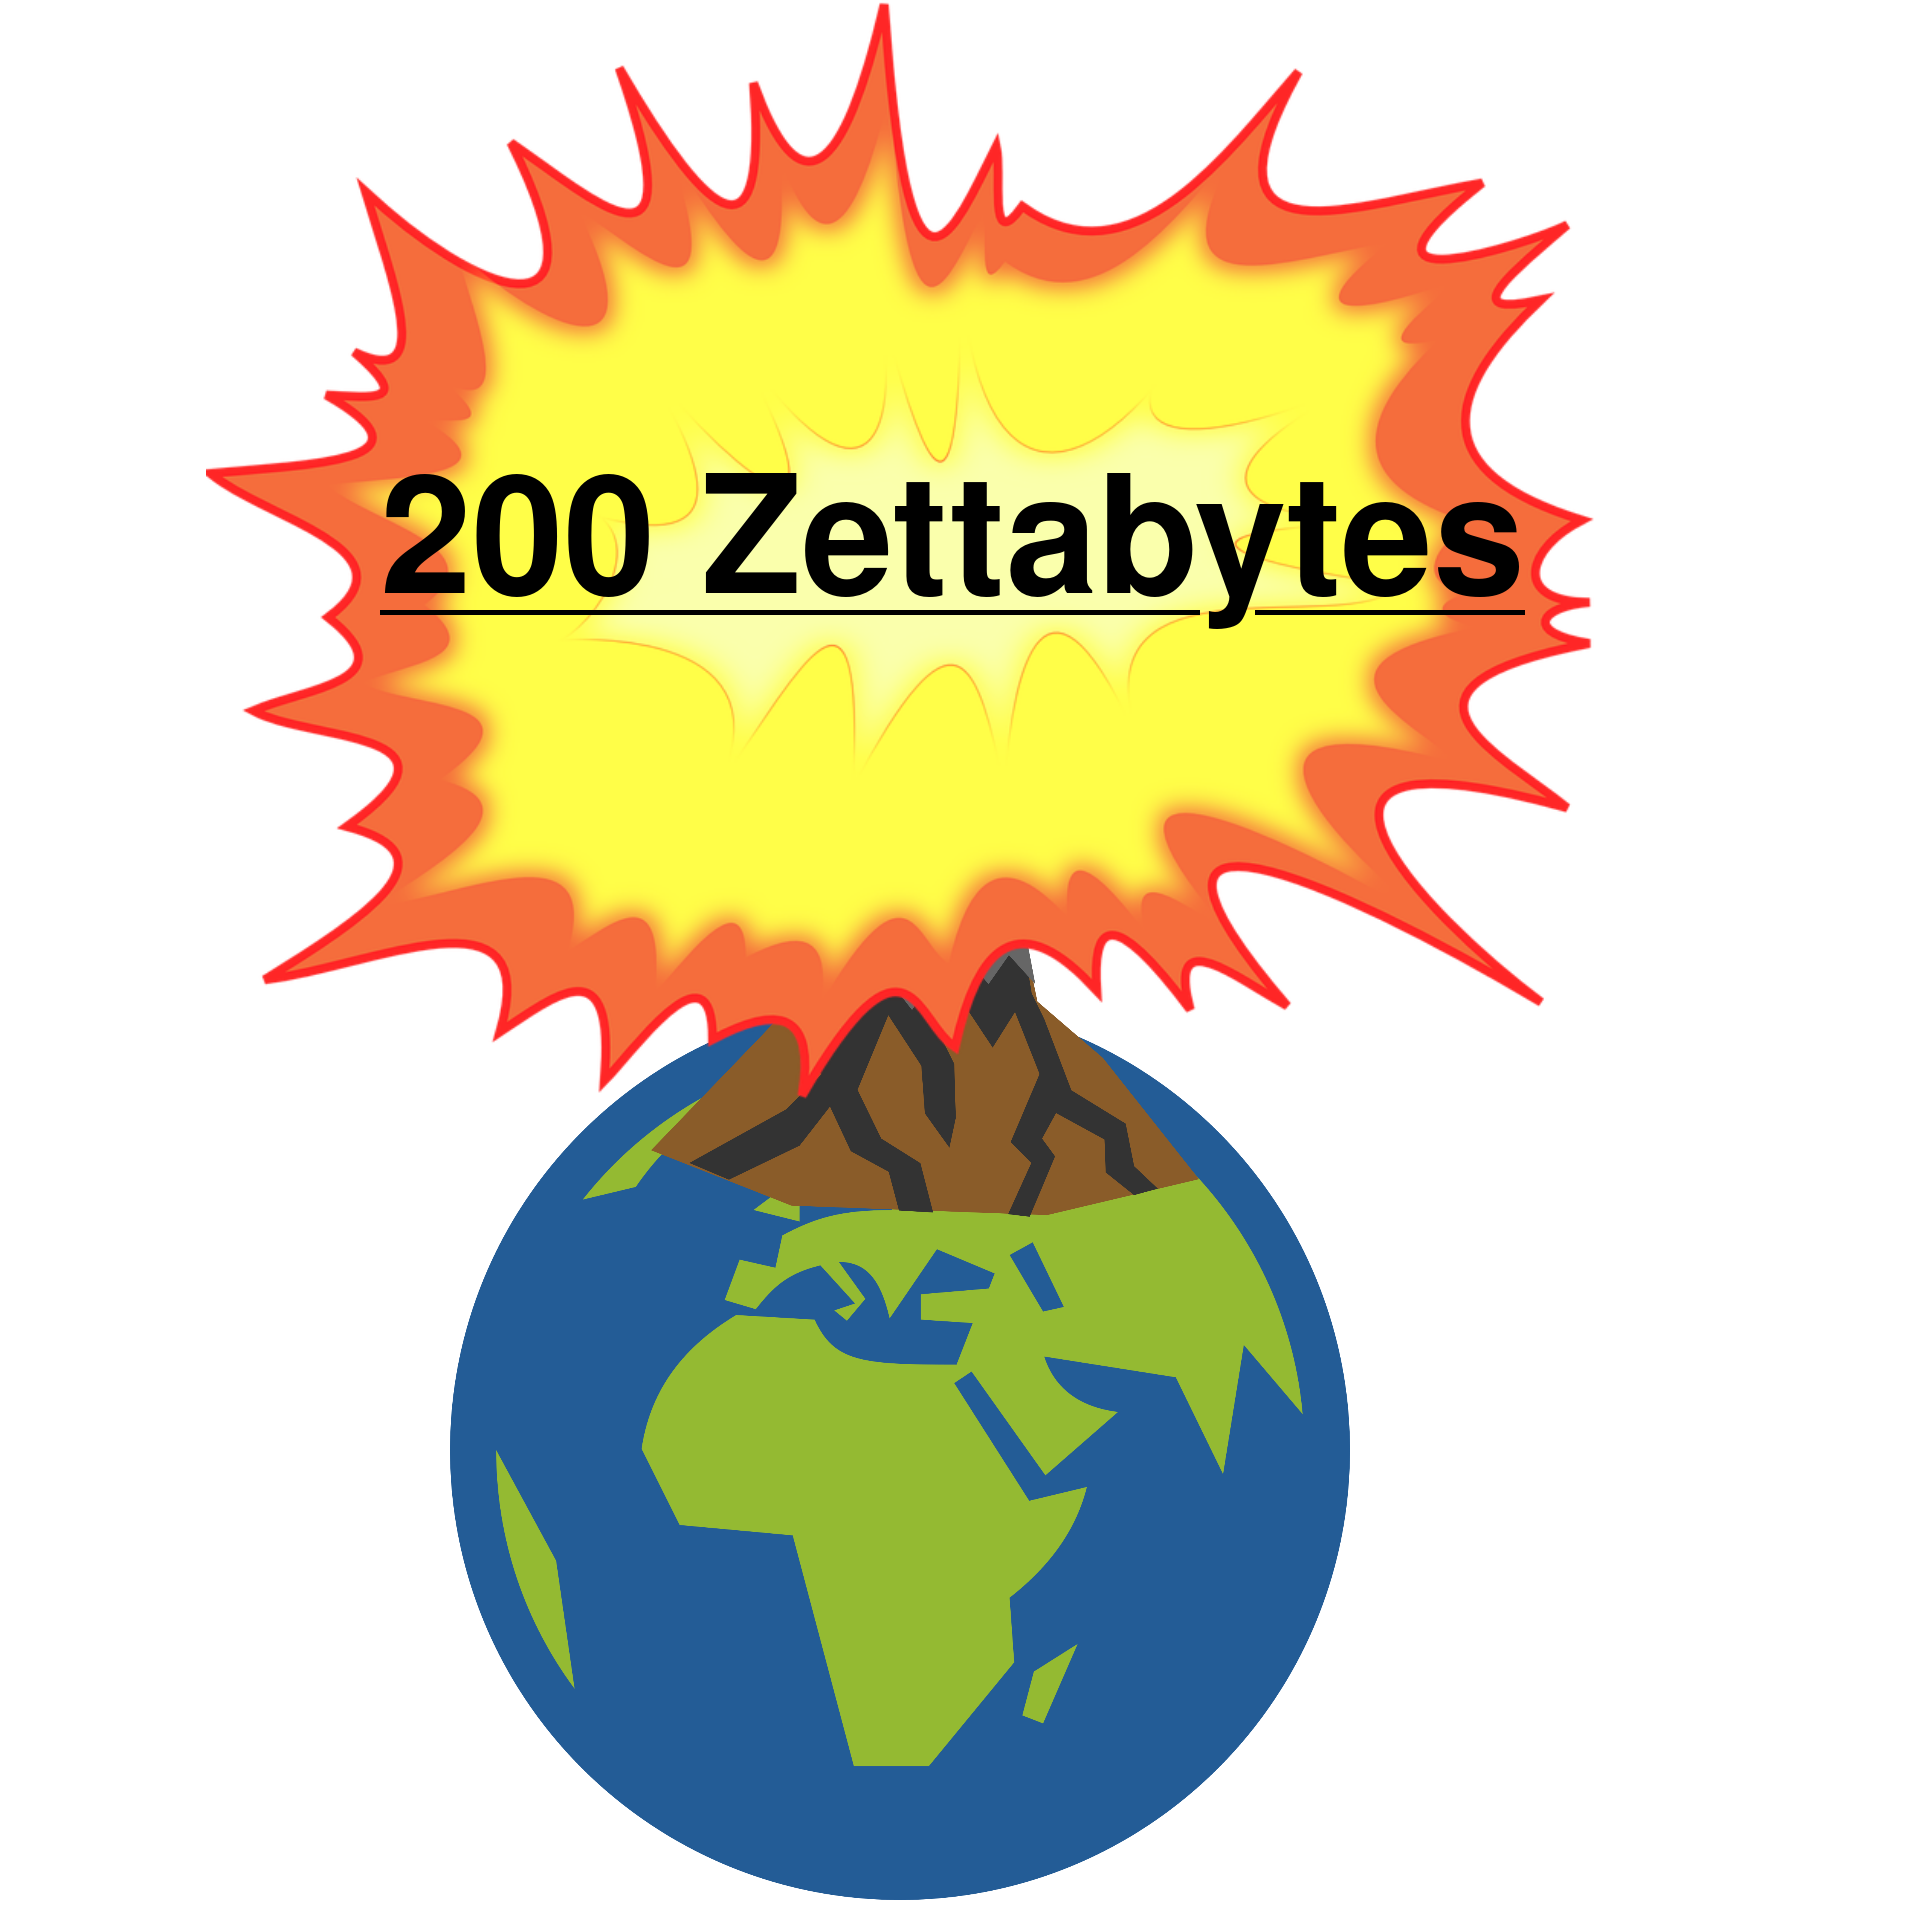
\includegraphics[width=0.9\textwidth]{resources/images/data-problem.png}
	\end{figure}
	\endgroup
\end{frame}

% page 2
% Perhaps the most prominent bottleneck in computer systems today is the one
% caused by the Von Neumann architecture. This architecture imposes restrictions
% on the location of data a CPU is able to operate on. Being it must either be
% in system memory, cache or a register. This prevents processors from directly
% operating on data provided by peripherals such as SSD flash storage. In
% addition the memory controller often has lower bandwidth then the interface
% used to connect peripherals while internally many flash devices togeteher are
% often able to saturate the bandwidth of peripheral interface as well. This
% leads to substantial bottlenecks primarily in enterprise SSD storage servers.
\begin{frame}{Von Neumann bottleneck}
	\begingroup
	\small
	\begin{figure}
		\centering
		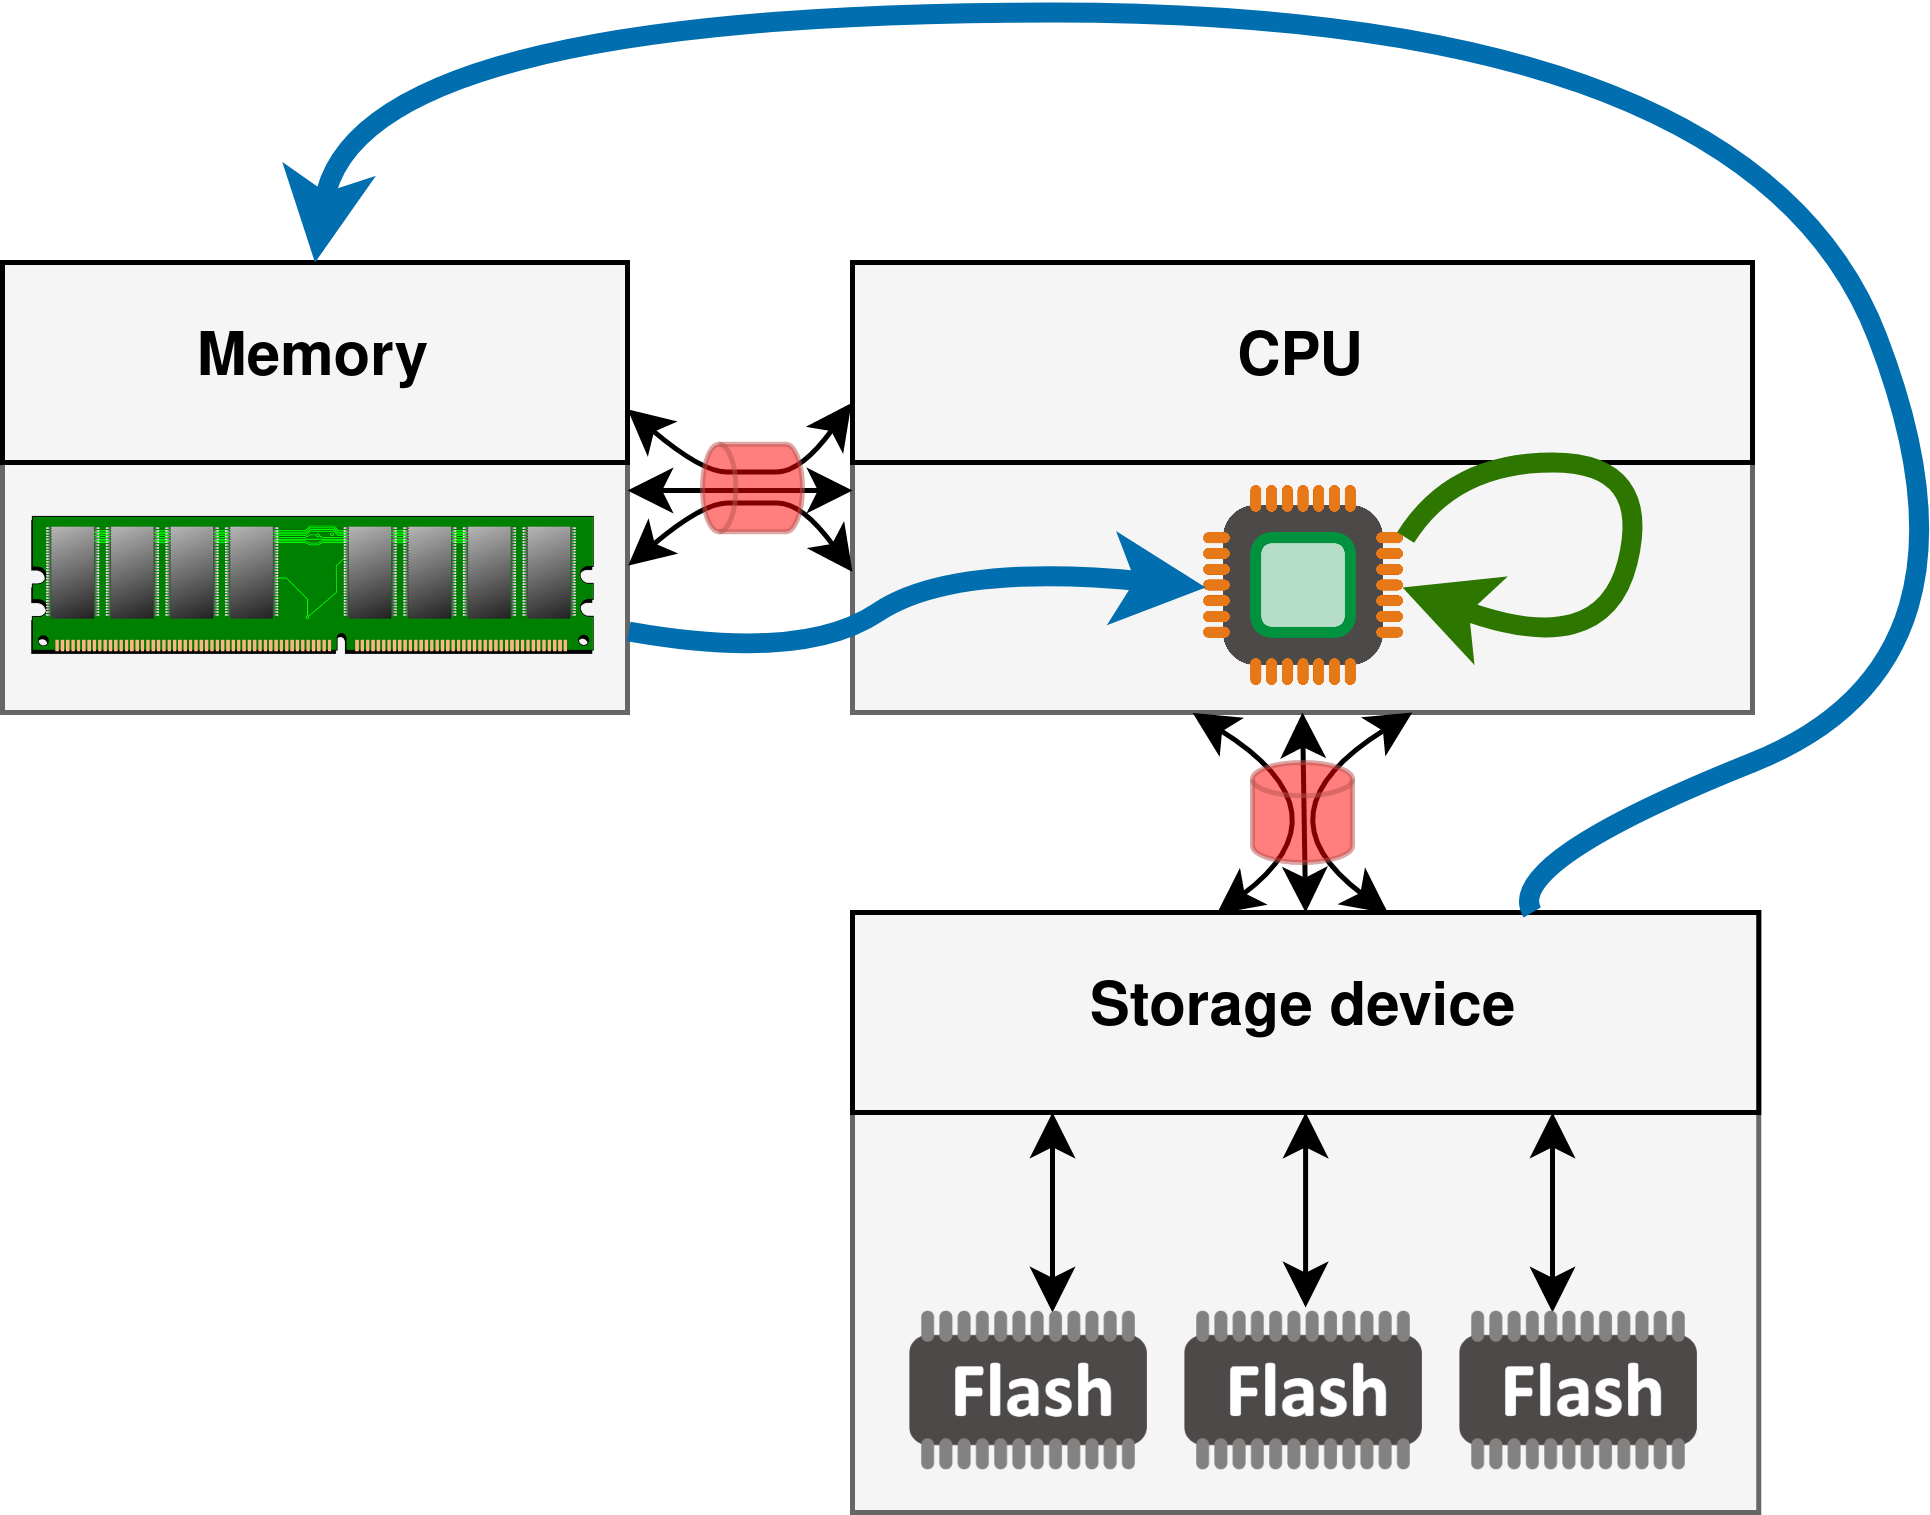
\includegraphics[width=0.7\textwidth]{resources/images/bottleneck.png}
	\end{figure}
	\endgroup
\end{frame}

% page 3
% With computational storage, flash storage devices are fitted with their own
% computational elements and memory. Often a combination of a regular processor
% combined with a field-programmable gate array, a subject we are unfortunately
% not able to cover further today. With computational storage the host system
% sends a user provided program along with metadata upon a particular I/O event
% or at the users descretion to the device for execution. All data from the
% storage device is thus moved internally an only the result of the execution is
% returned to the host for further processing. While the result still has to be
% moved to system memor, the computation often is reductive in nature, reducing
% the amount of bandwidth occupied on the perihperal interfaces and memory
% controller.
\begin{frame}{Computational Storage Devices (CSx)s}
	\begingroup
	\small
	\begin{figure}
		\centering
		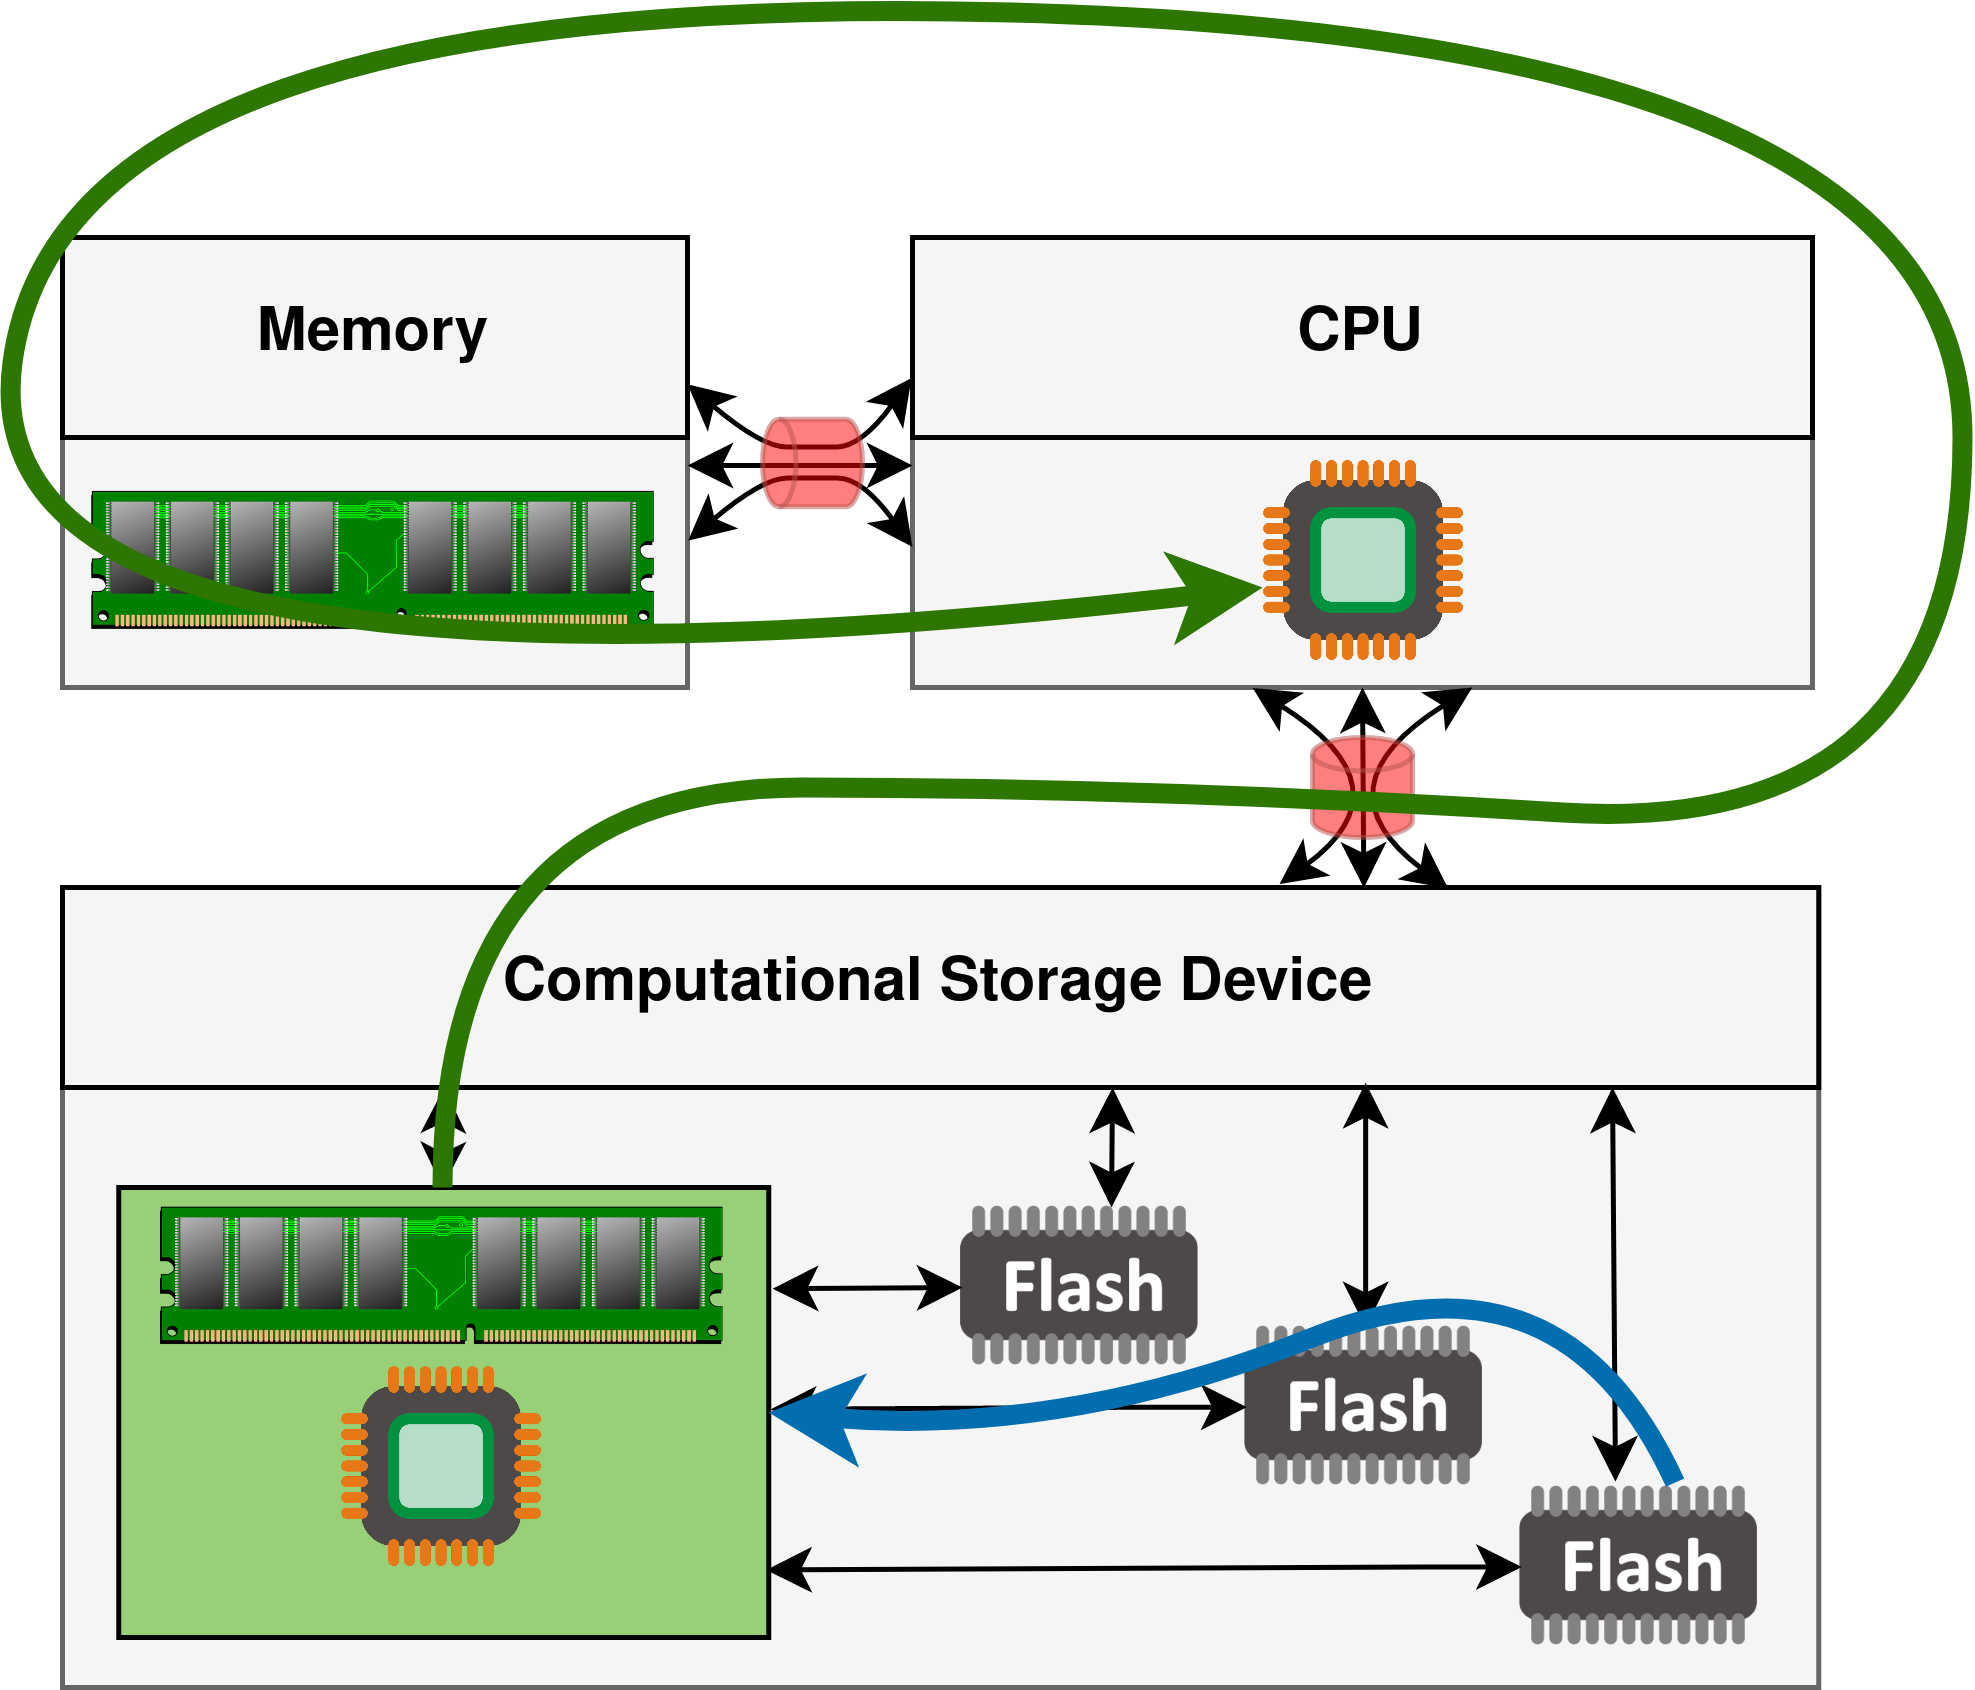
\includegraphics[width=0.7\textwidth]{resources/images/csd.png}
	\end{figure}
	\endgroup
\end{frame}

% page 4
% But such a heregoenous distributed system comes with many challenges and
% complexities. For filesystems providing both offloaded and regular user access
%, further called _hybrid_ filesystem these challenges resolve primary around
% consistency. Preventing that parts of files being read are already overwritten
% or multiple writes are going to the same parts of a file.

% Other related work trying to address this, INSIDER - one time translation
% BlockNDP, designed for filesystem support but not implemented
% Metal FS, supports regular and offloaded access but overwrites UNIX pipes
% behavior.
\begin{frame}{Challenges}
	\begingroup
	\small
	\begin{figure}
		\centering
		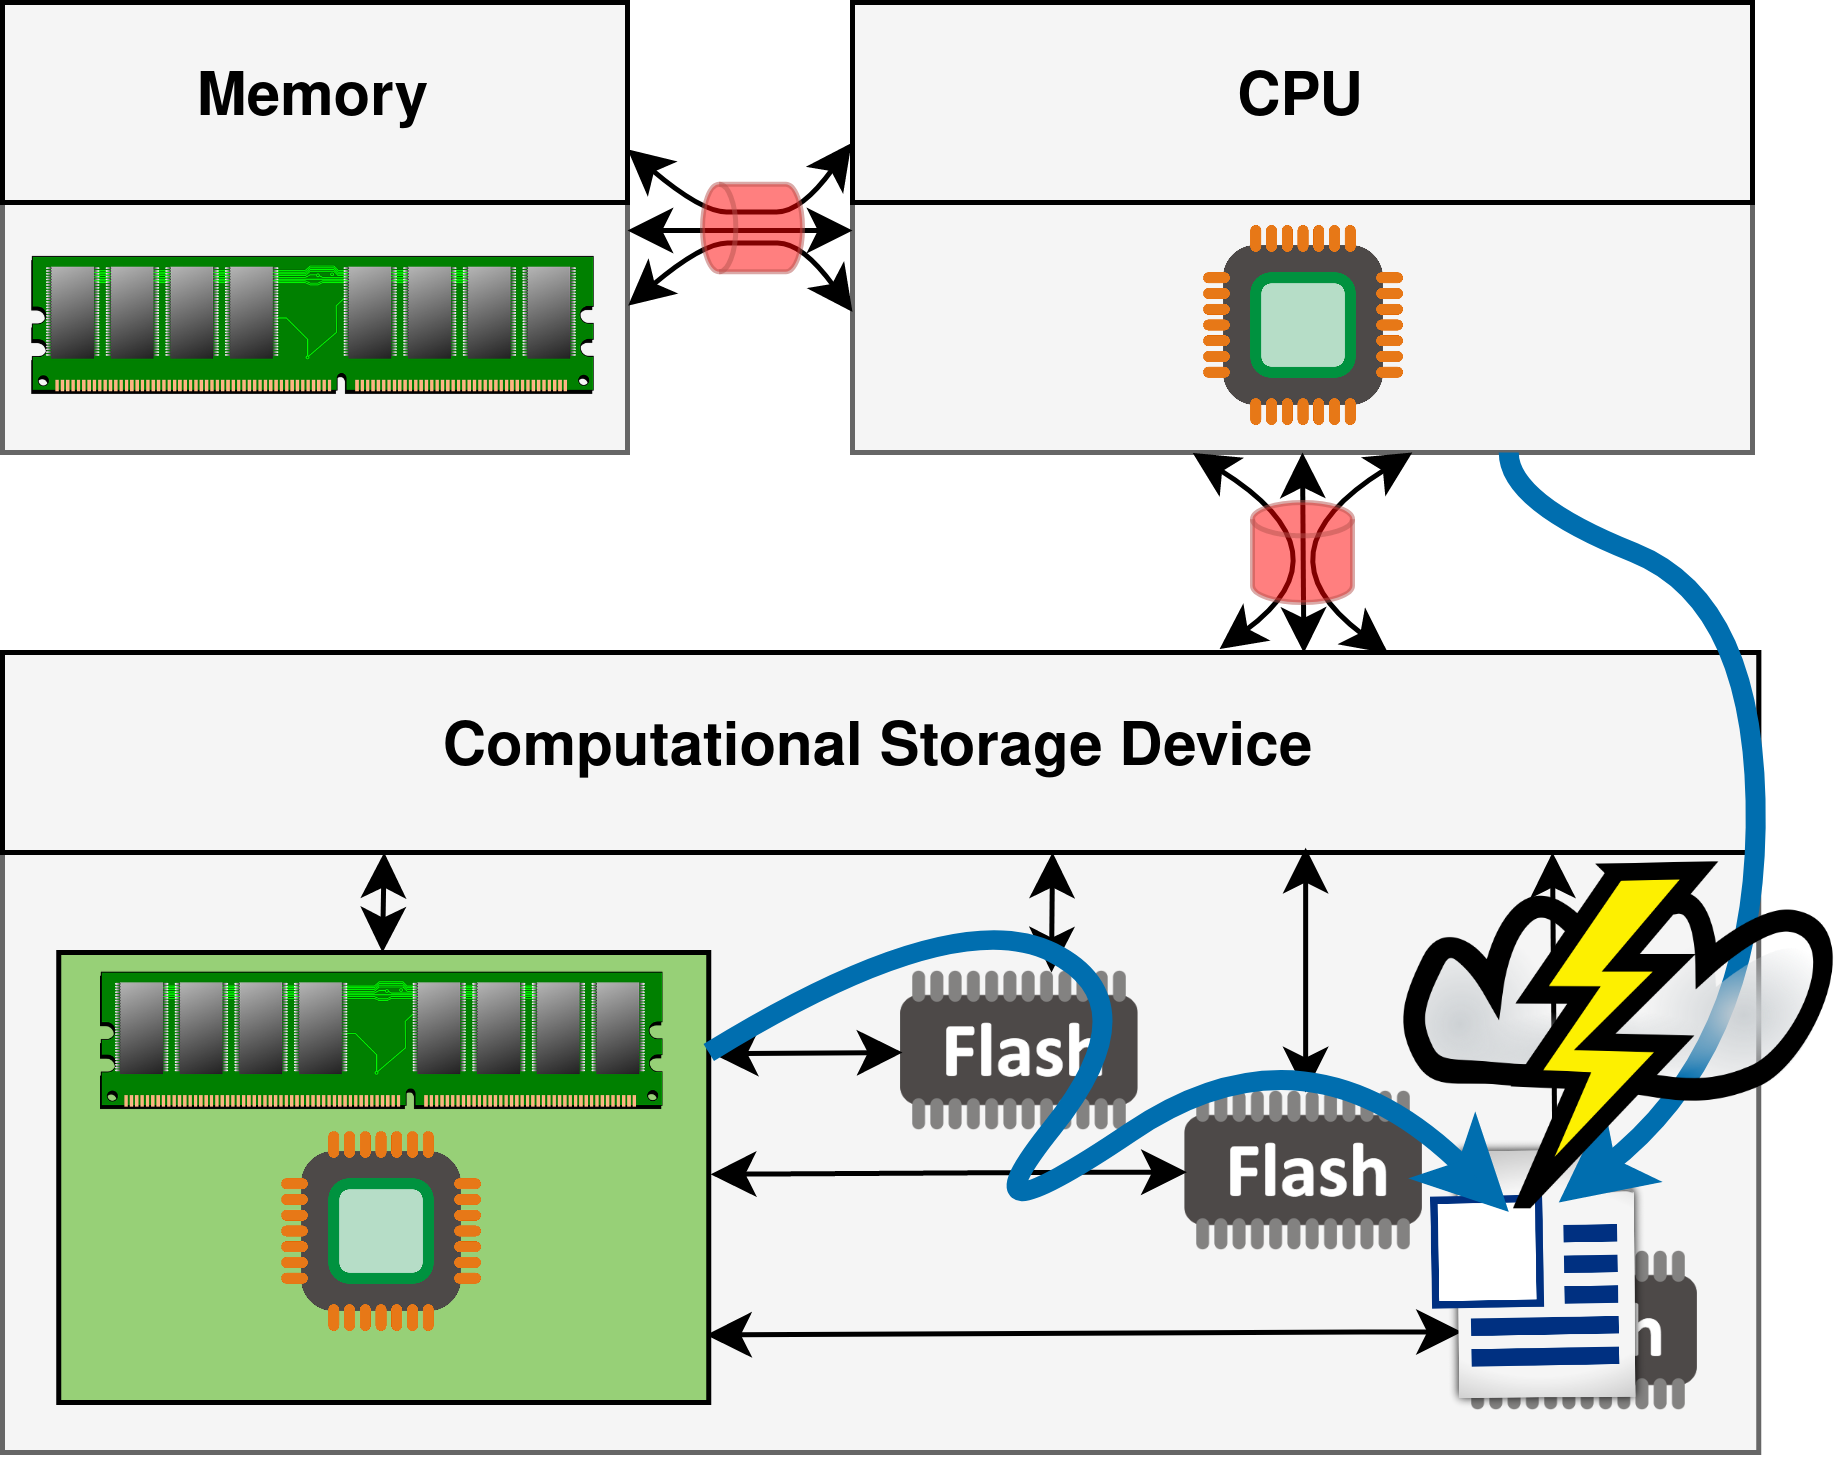
\includegraphics[width=0.7\textwidth]{resources/images/challenges.png}
	\end{figure}
	\endgroup
\end{frame}

% page 5
% 
\begin{frame}{Research Questions}
	\begingroup
	\small
		How to create a filesystem providing consitent regular access concurrent
		with Computational Storage offloading (\textit{hybrid}) support?
	\begin{itemize}
		\item How to register CSx compute kernels using existing operating 
			  system APIs?
  		\item How to differentiate individual users, files and I/O operations in
			  relation to their CSx compute kernel?
		\item Can a \textit{hybrid} filesystem reduce the host load for
              asynchronous applications?
	\end{itemize}
	\endgroup
\end{frame}

% page 6
% 
\begin{frame}{Design}
	\begingroup
	\small
	
	\FourQuad%
		{\centering Modules \& Interfaces
		\begin{figure}
			\centering
			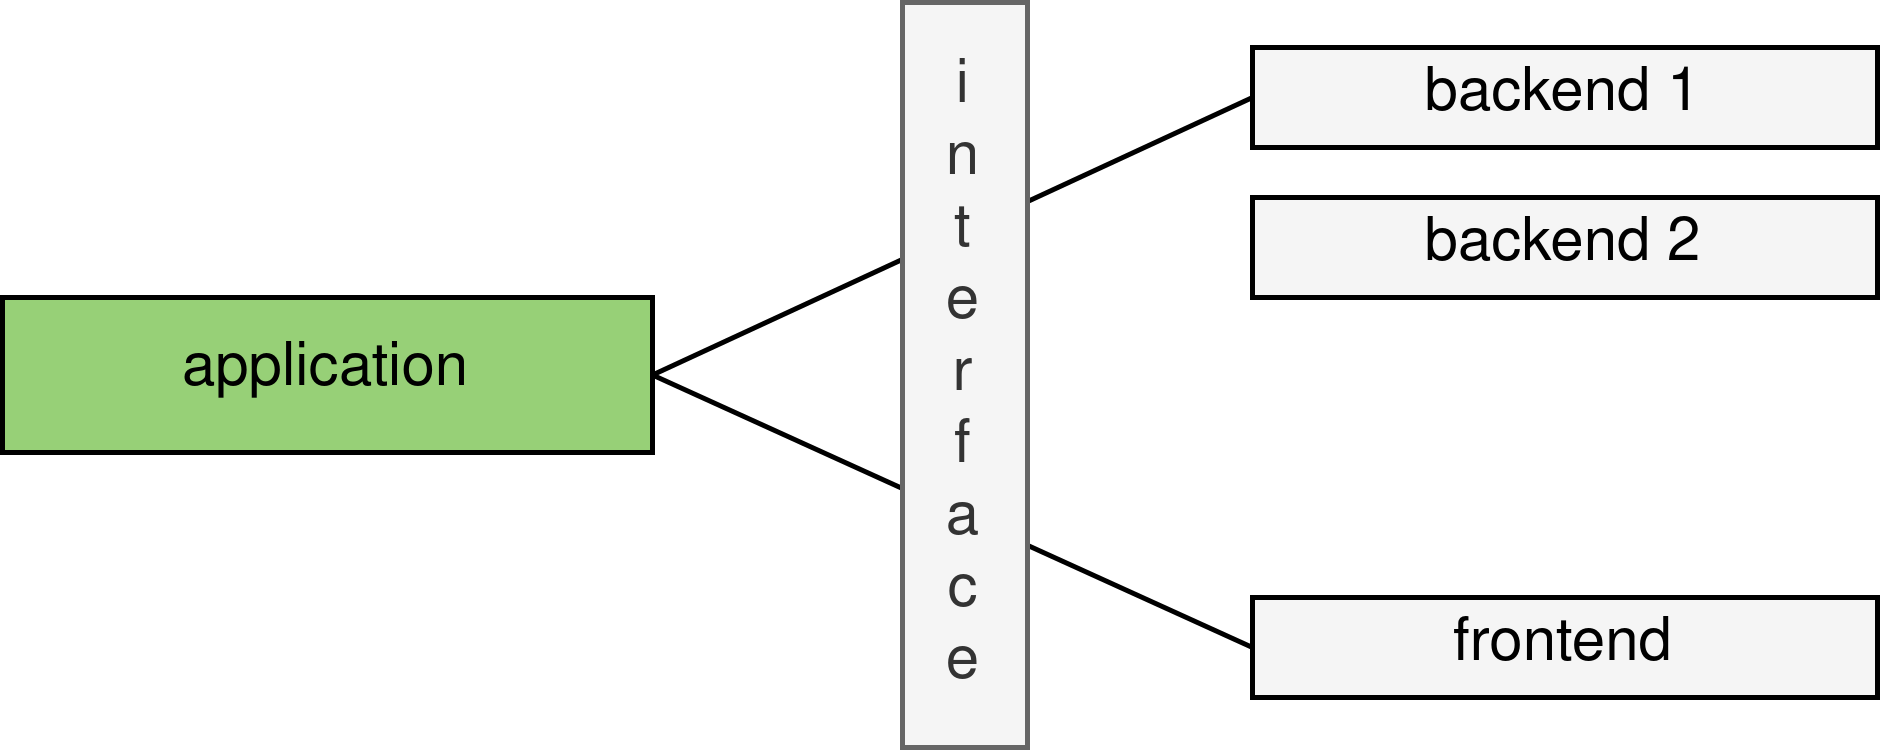
\includegraphics[width=1.0\textwidth]{resources/images/modules-interfaces.png}
		\end{figure}
		}
		{\centering Log-Structured Filesystem (LFS)$^1$
		\begin{figure}
			\centering
			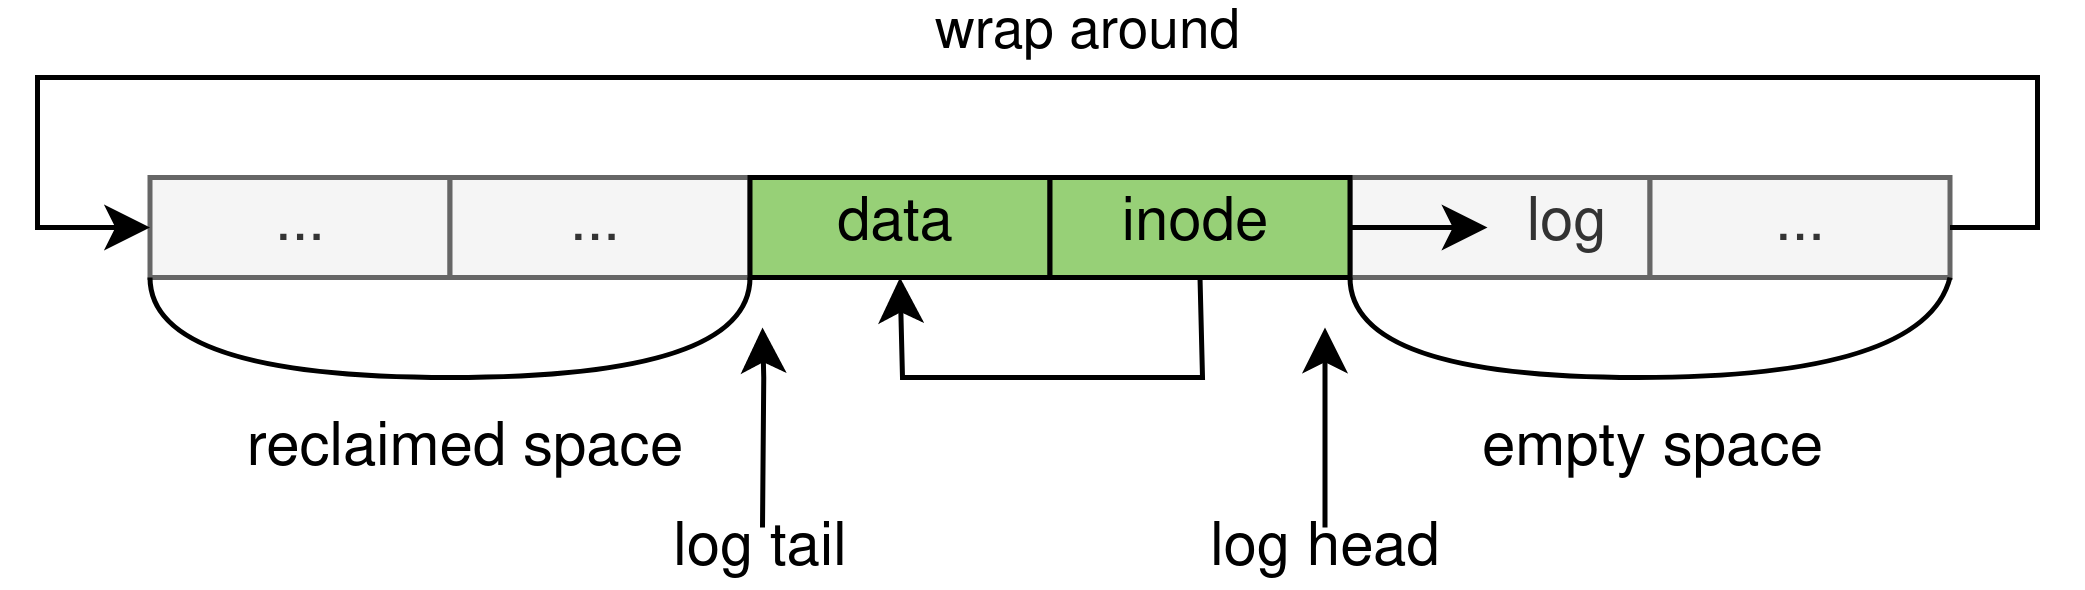
\includegraphics[width=0.9\textwidth]{resources/images/lfs-example.png}
		\end{figure}
		}
		{\centering Zoned Namespaces (ZNS)
		\begin{figure}
			\centering
			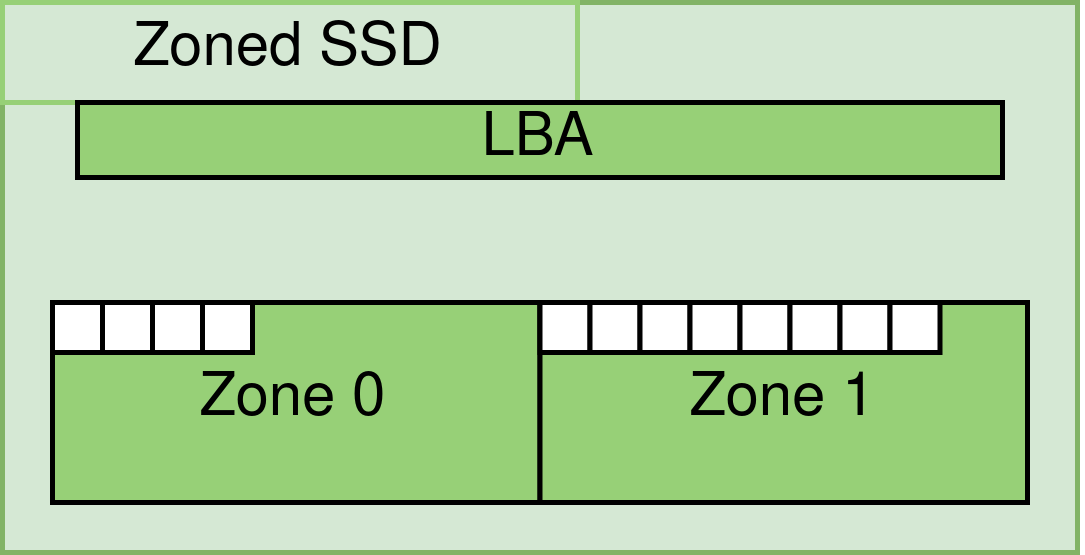
\includegraphics[width=0.7\textwidth]{resources/images/zns-simple.png}
		\end{figure}
		}
		{\centering Extended Attributes (xattr)
		\begin{figure}
			\centering
			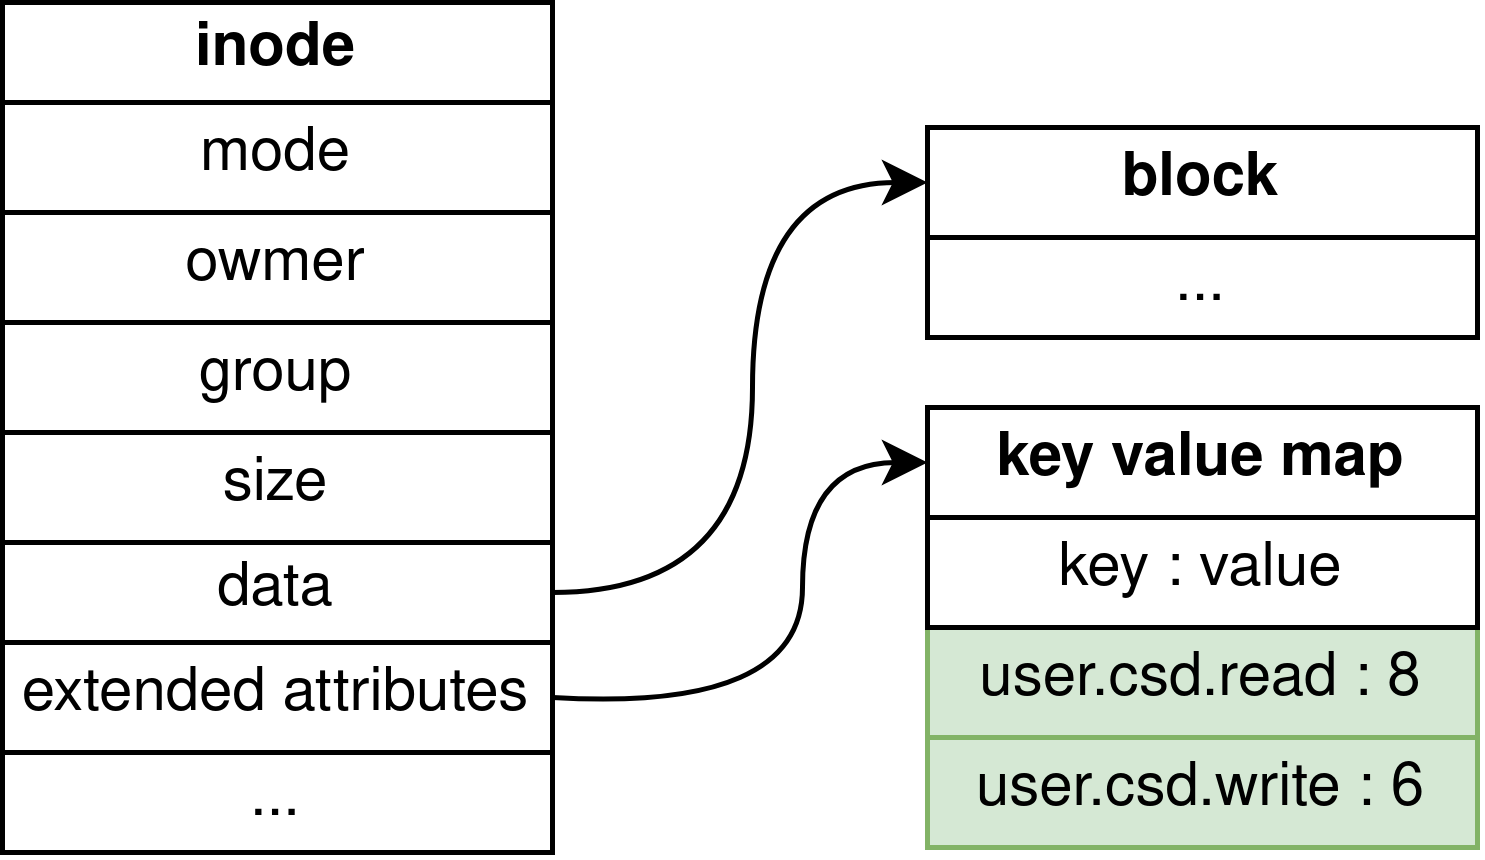
\includegraphics[width=0.7\textwidth]{resources/images/xattr-inode.png}
		\end{figure}
		}
		\\
		\textit{\tiny $^{1}$The design and implementation of a Log-structured File System \\}
	\endgroup
\end{frame}

% page 7
% 
\begin{frame}{Design: Architecture Independent Kernels}
	\begingroup
	\begin{figure}
		\centering
		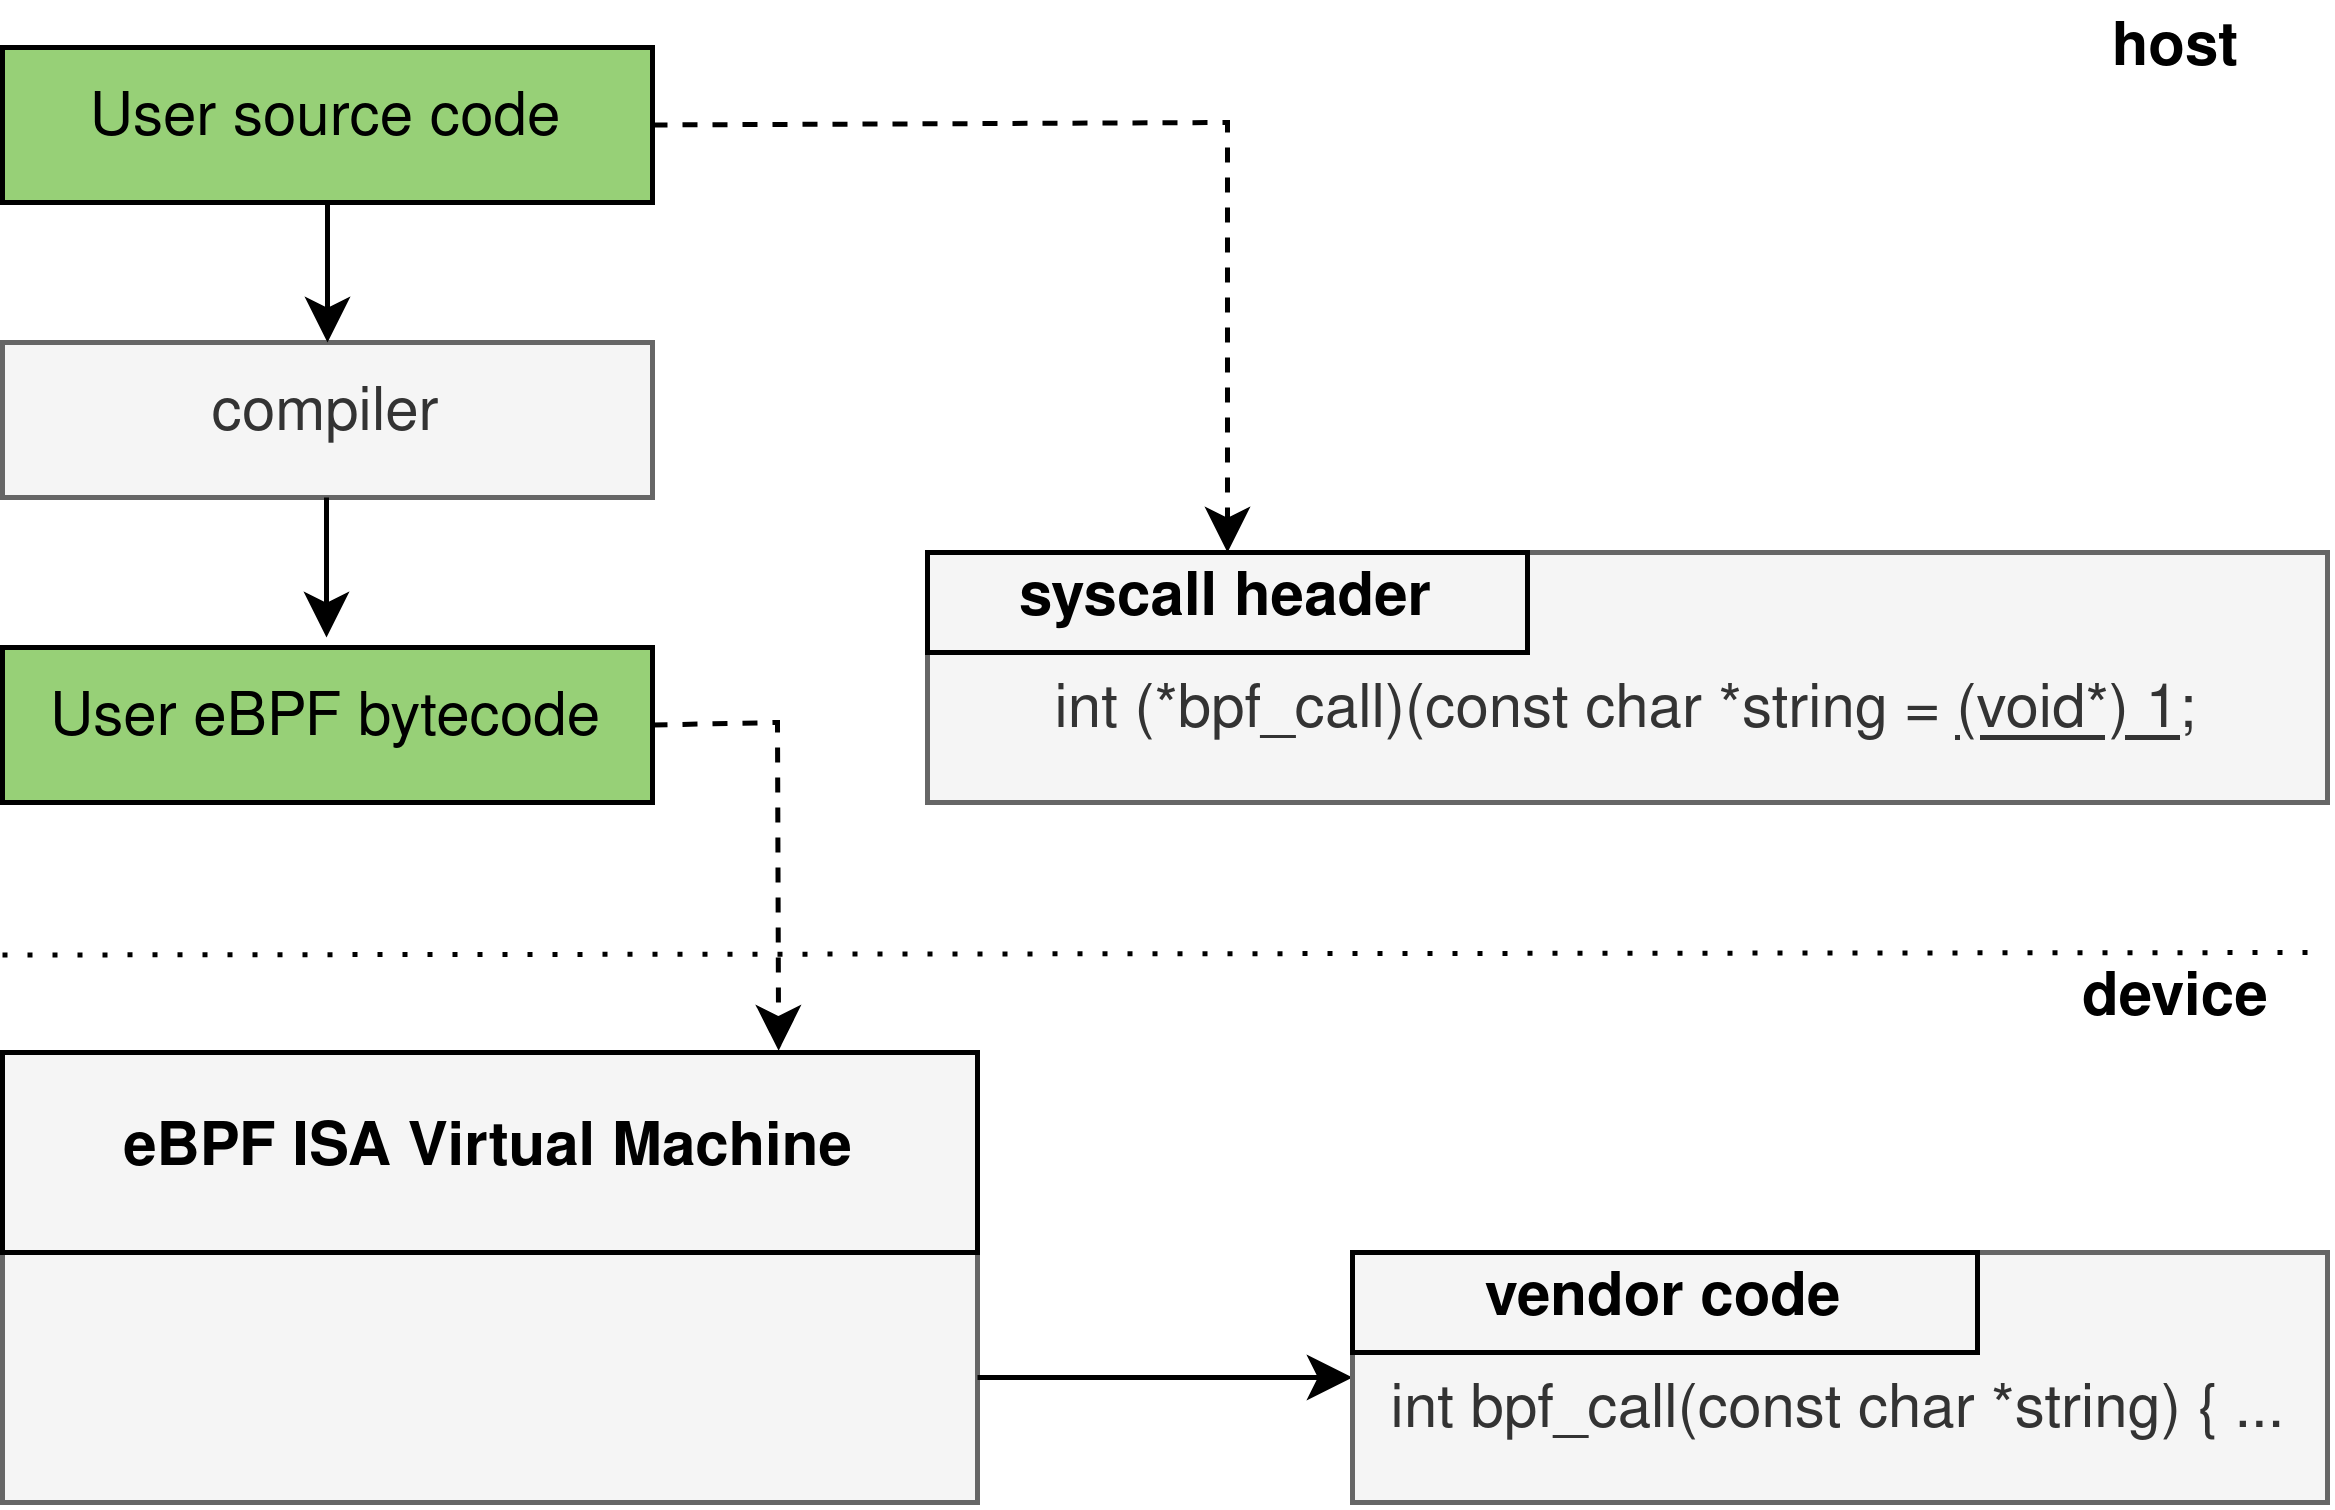
\includegraphics[width=0.8\textwidth]{resources/images/ubpf-medium-design.png}
	\end{figure}
	\endgroup
\end{frame}

% page 8
% \begin{frame}{Design: Interfaces \& Modules}
% 	\begingroup
% 	\small

% 	\endgroup
% \end{frame}

% page 9
\begin{frame}{Design: ZNS + LFS}
	\begingroup
	\small
	\begin{figure}[h]
		\centering
		% \begin{subfigure}{0.5\textwidth}
			%   \centering
			  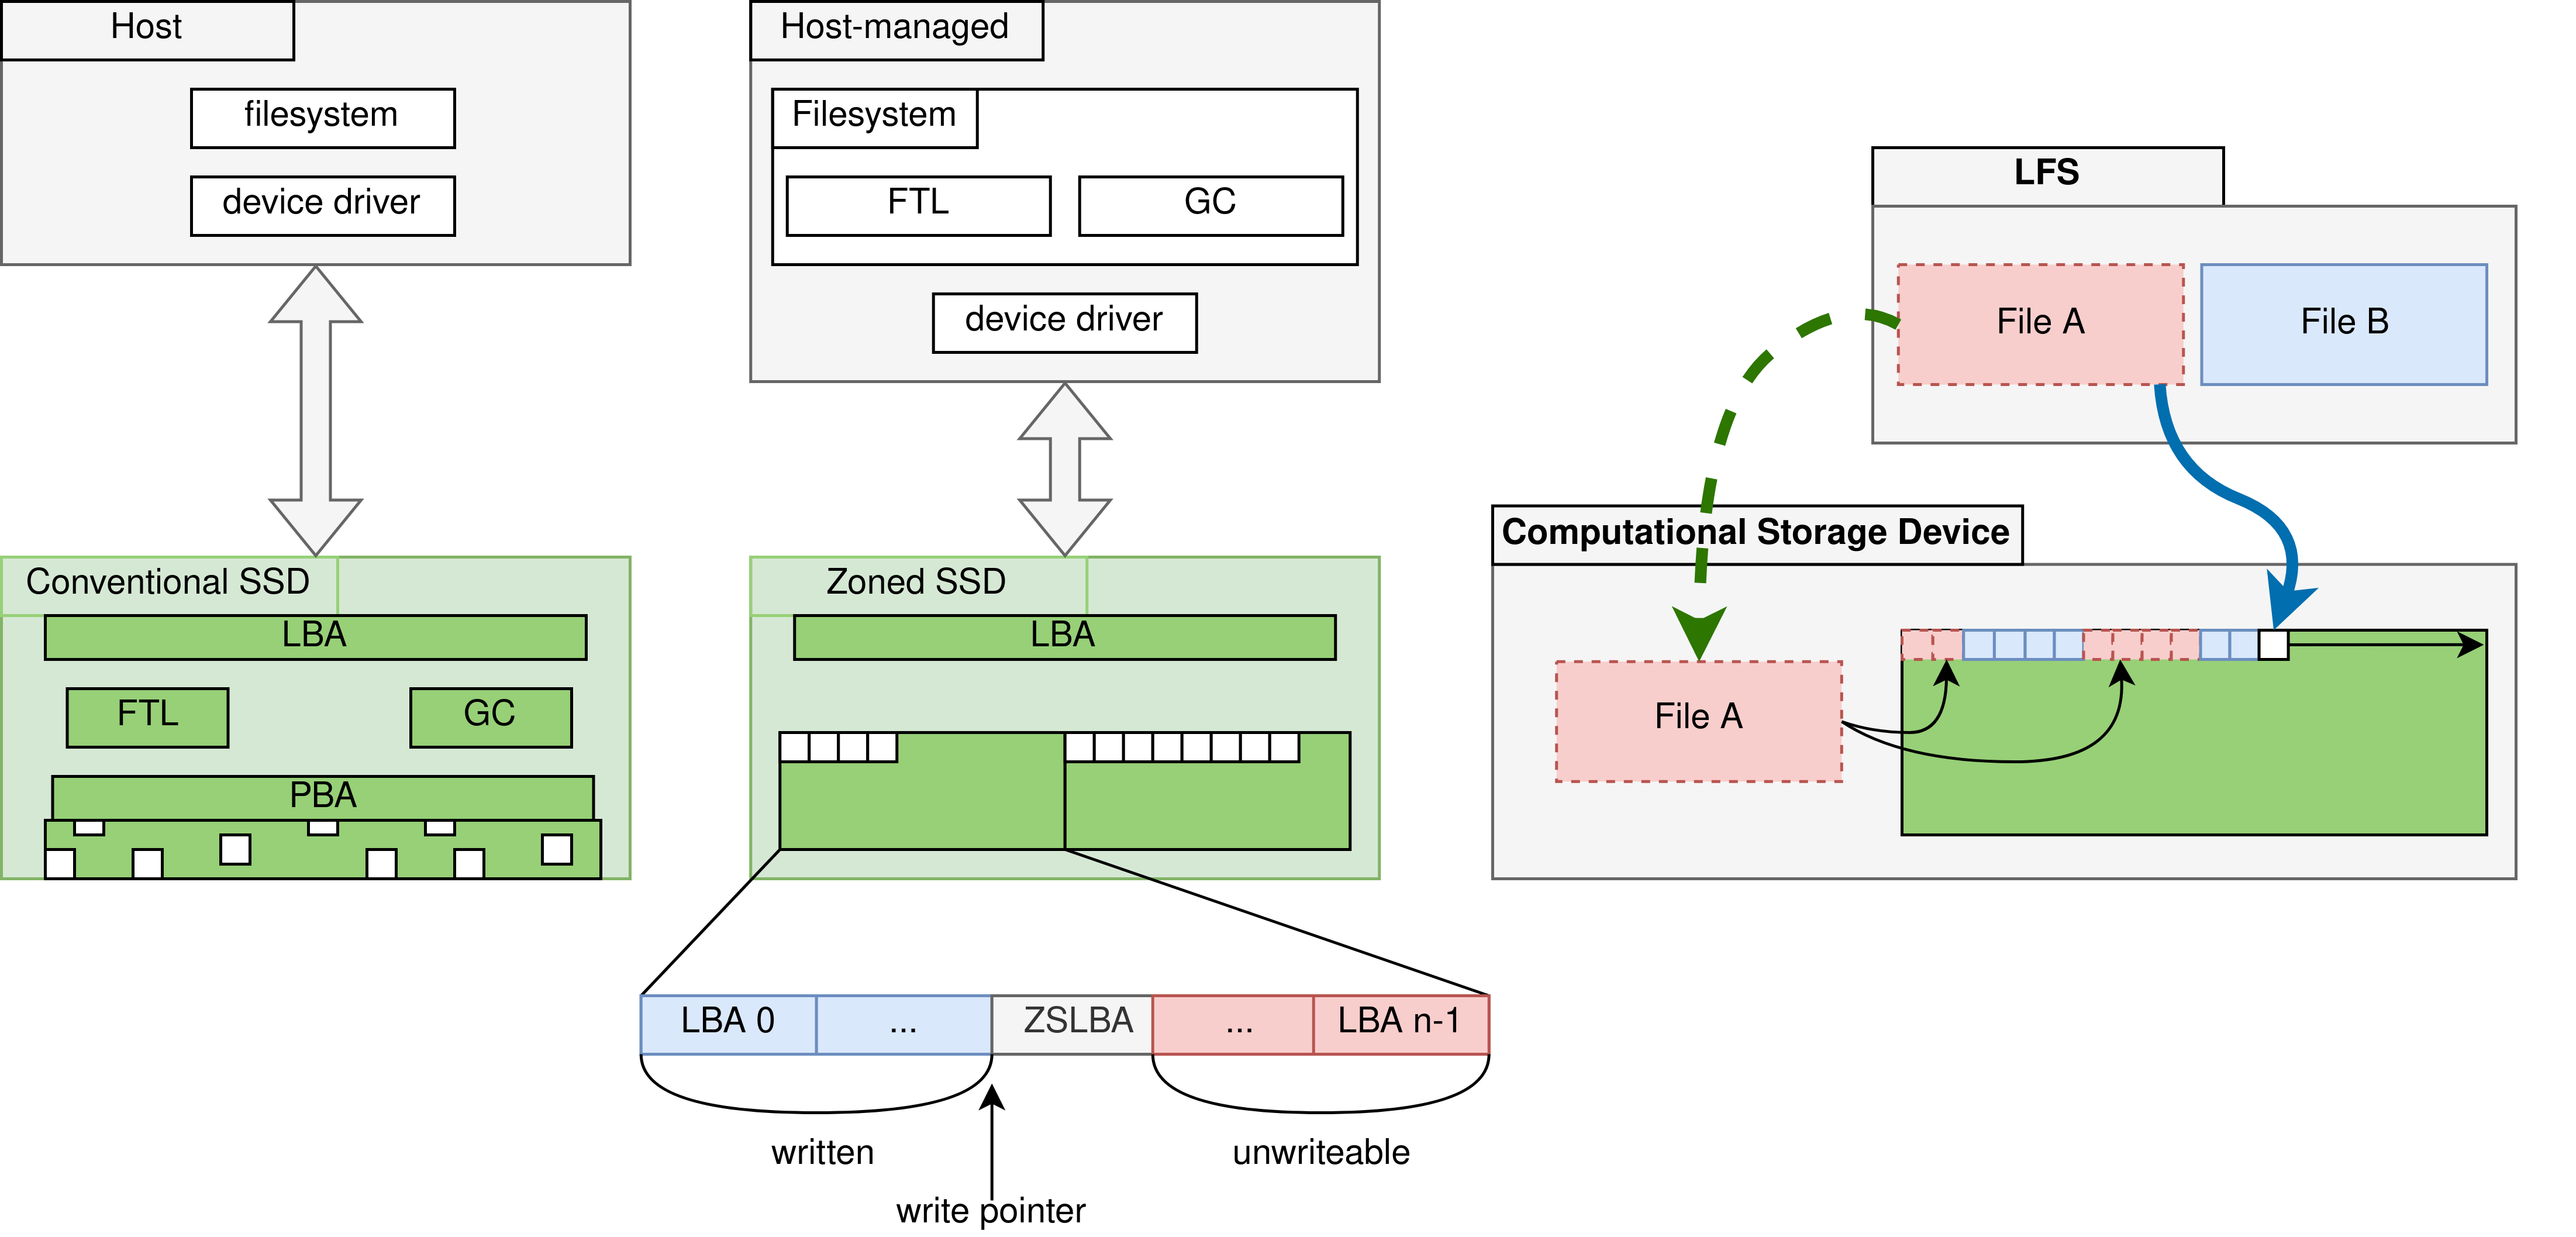
\includegraphics[width=1.0\linewidth]{resources/images/zns-lfs.png}
		% \end{subfigure}%
		% \begin{subfigure}{0.5\textwidth}
		% 	  \centering
		% 	  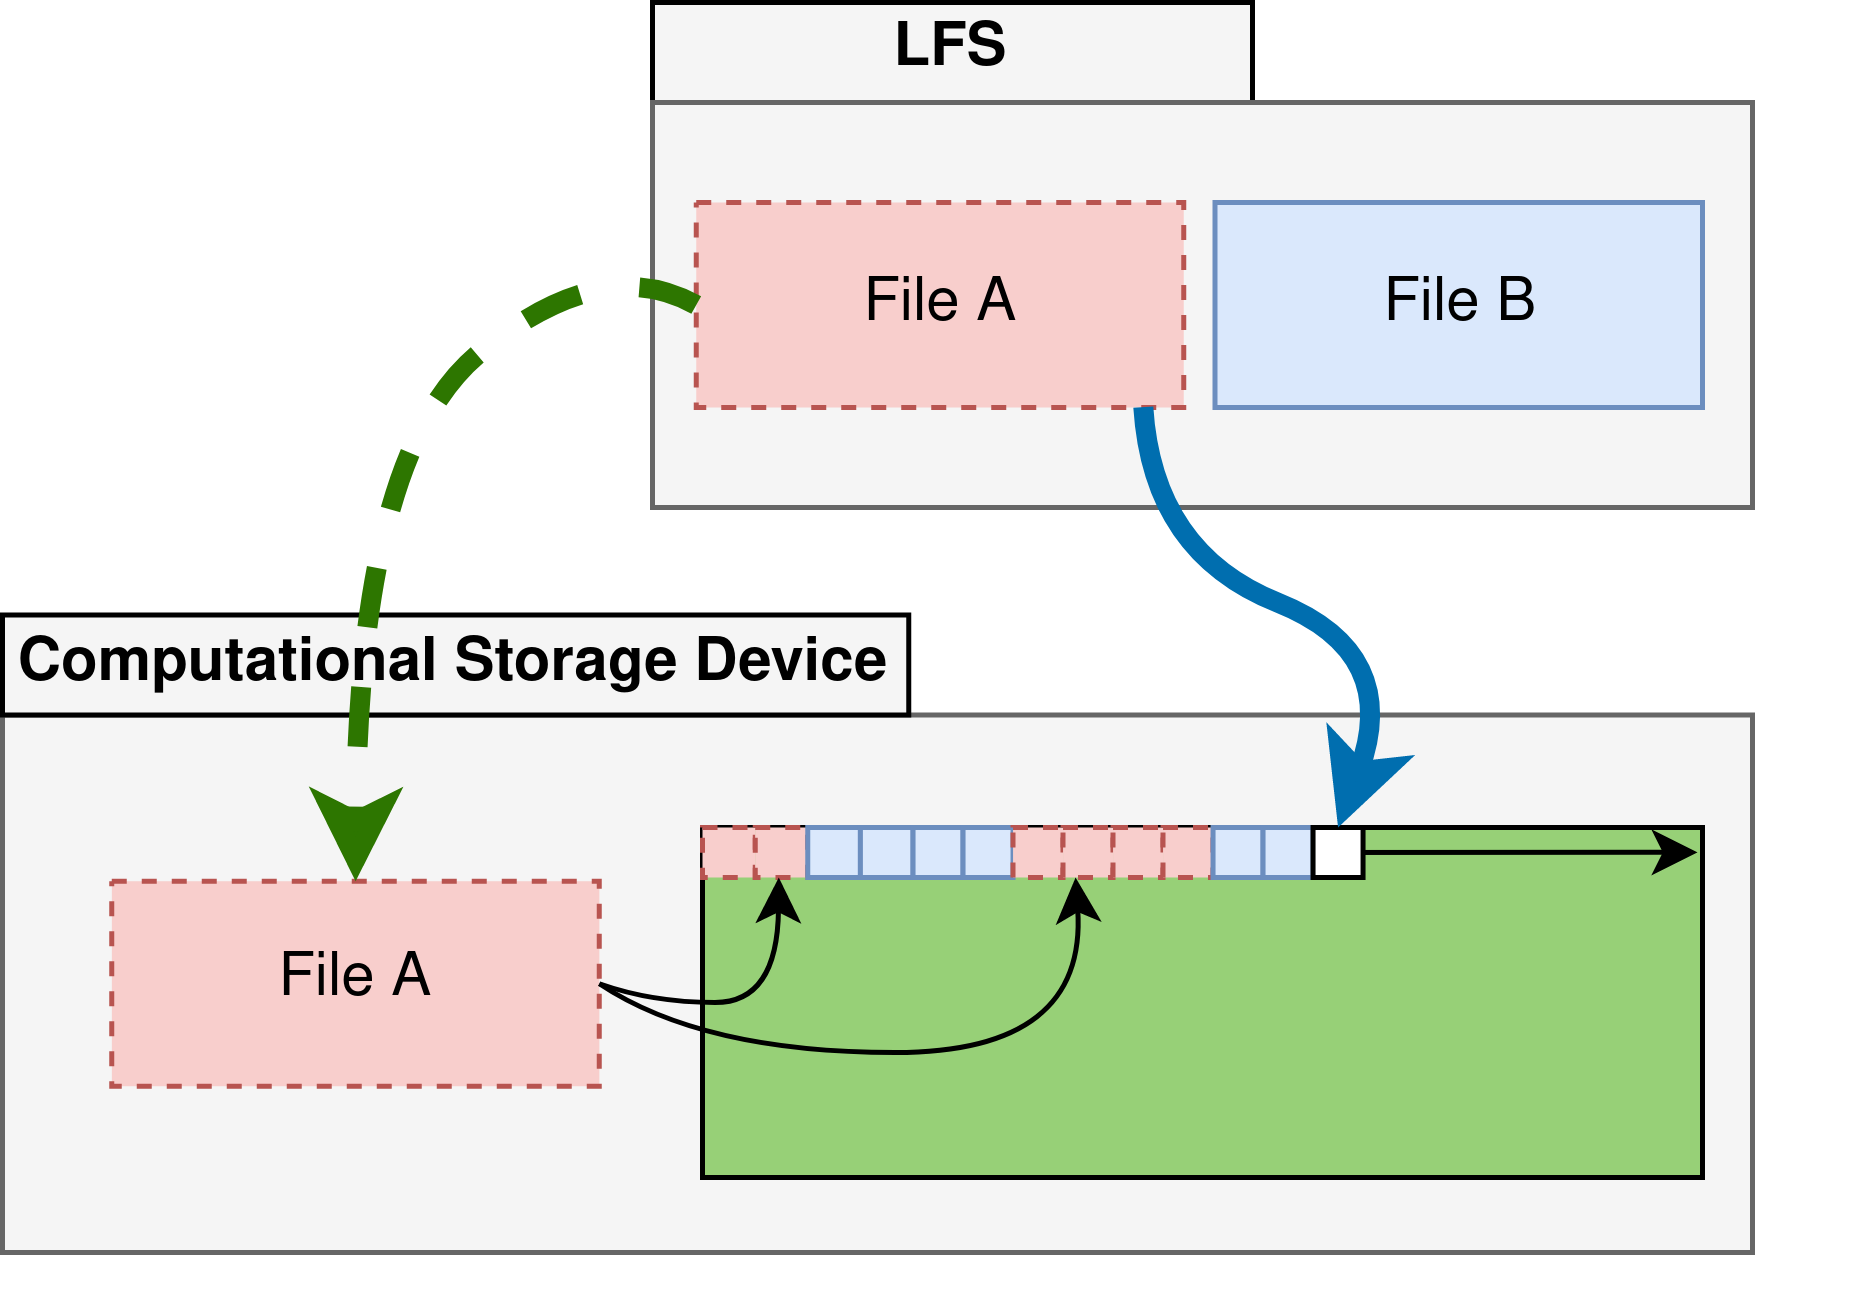
\includegraphics[width=0.9\linewidth]{resources/images/lfs.png}
		% \end{subfigure}
	\end{figure}
	\textit{\tiny $^{2}$NVM Express Zoned Namespace Command Set Specification 1.1b - https://nvmexpress.org/developers/nvme-command-set-specifications/}
	\endgroup
\end{frame}

% page 10
\begin{frame}{Orientation}
	\begingroup
	\small Next slides, implementation...
	\begin{itemize}
		\item Filesystem drive layout
		\item Filesystem datastructures
		\item How offloading is achieved using existing OS APIs
		\item How to differentiate individual users and registered kernels on files
		\item Evaluation...
	\end{itemize}
	\endgroup
\end{frame}

% page 11
\begin{frame}{Implementation: Drive Layout}
	\begingroup
	\small
	\begin{figure}[h]
		\centering
		% \begin{subfigure}{0.5\textwidth}
			%   \centering
			  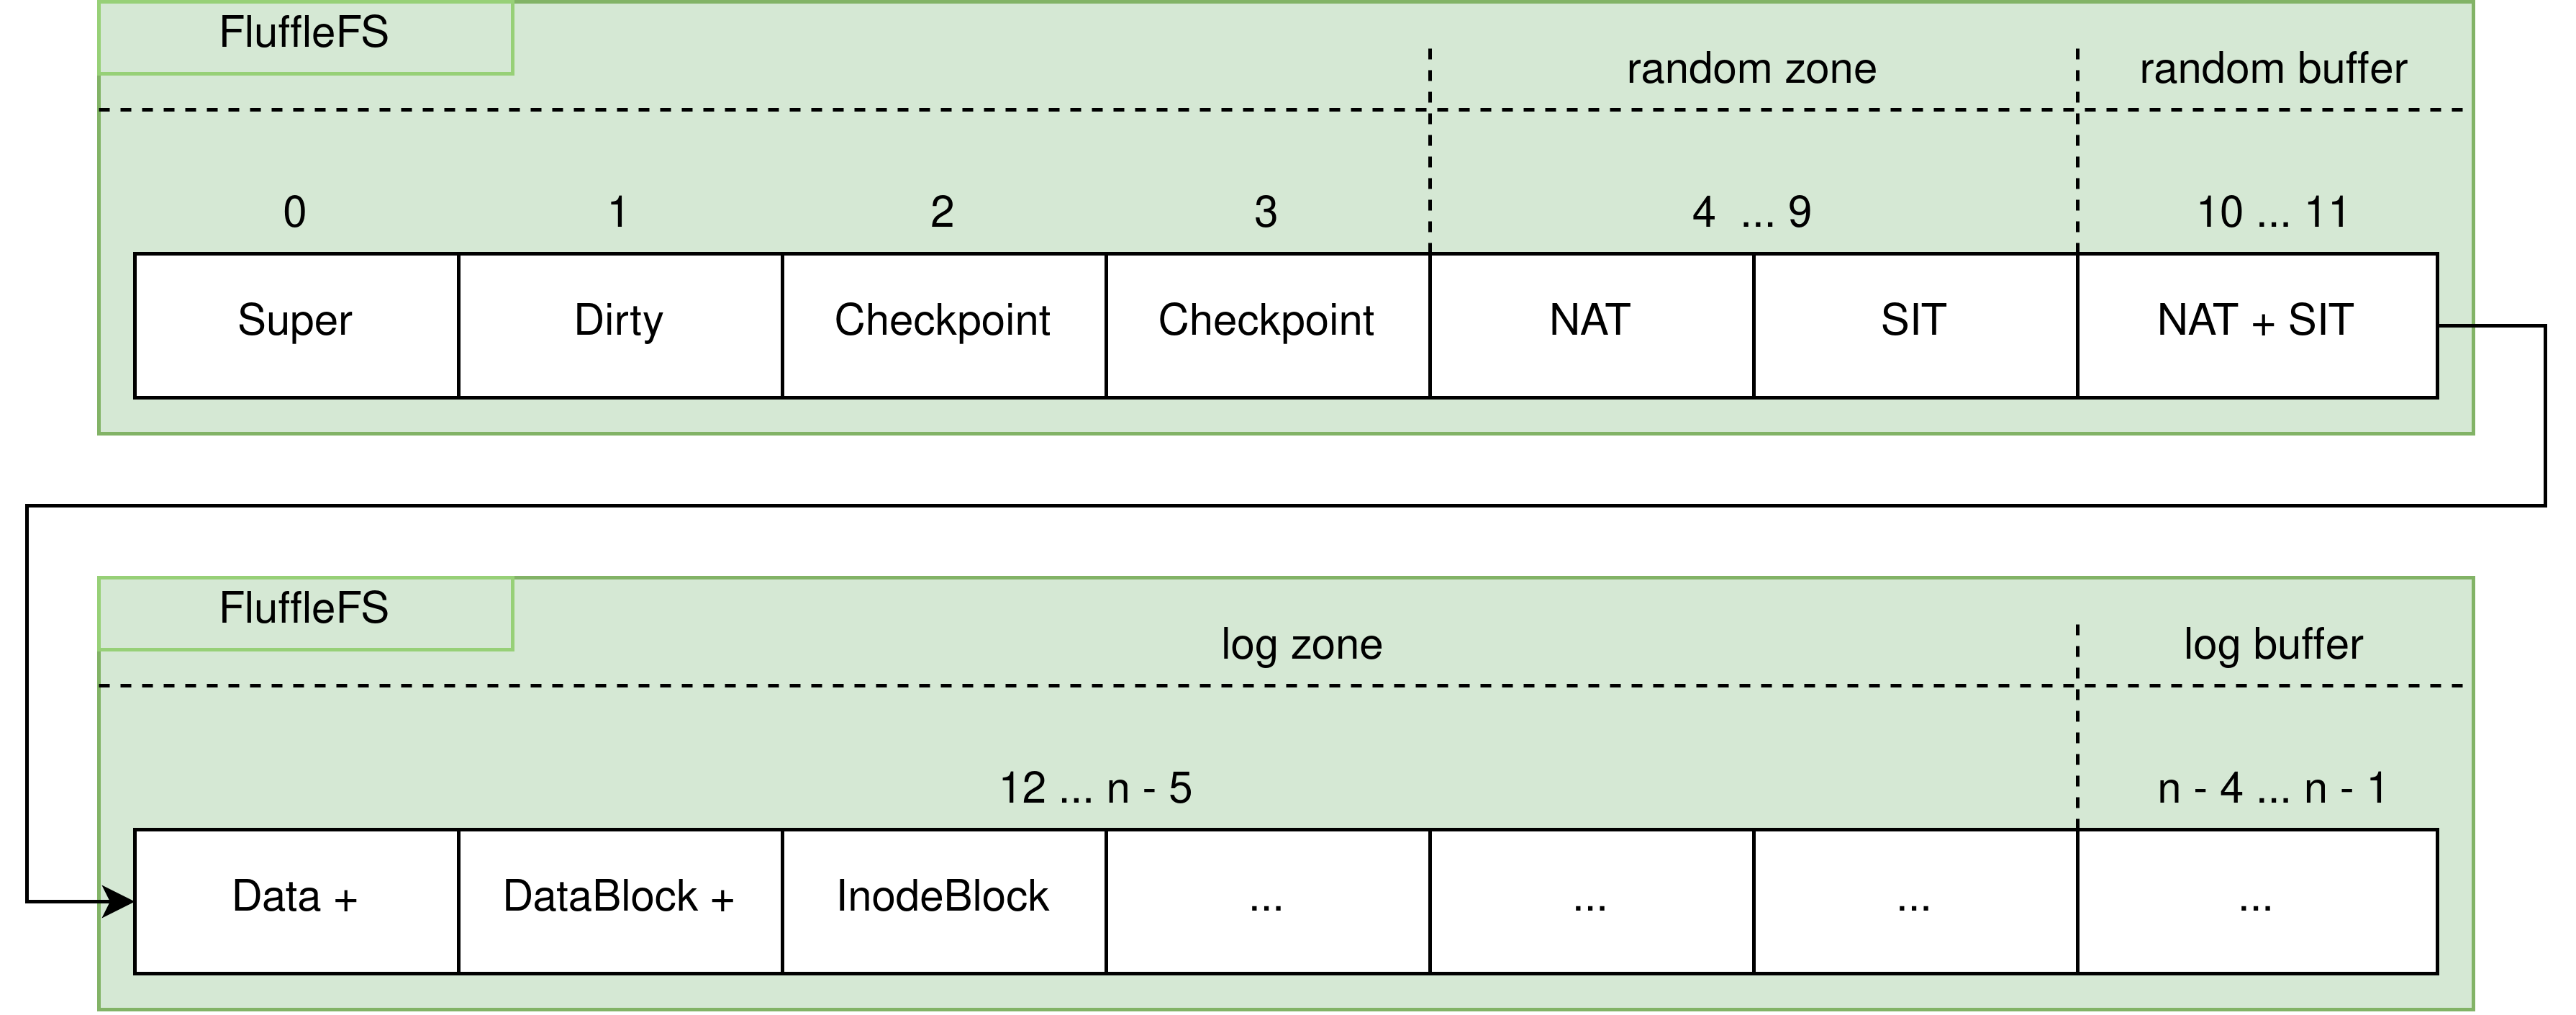
\includegraphics[width=1.0\linewidth]{resources/images/fluffle-layout-complete.png}
		% \end{subfigure}%
		% \begin{subfigure}{0.5\textwidth}
		% 	  \centering
		% 	  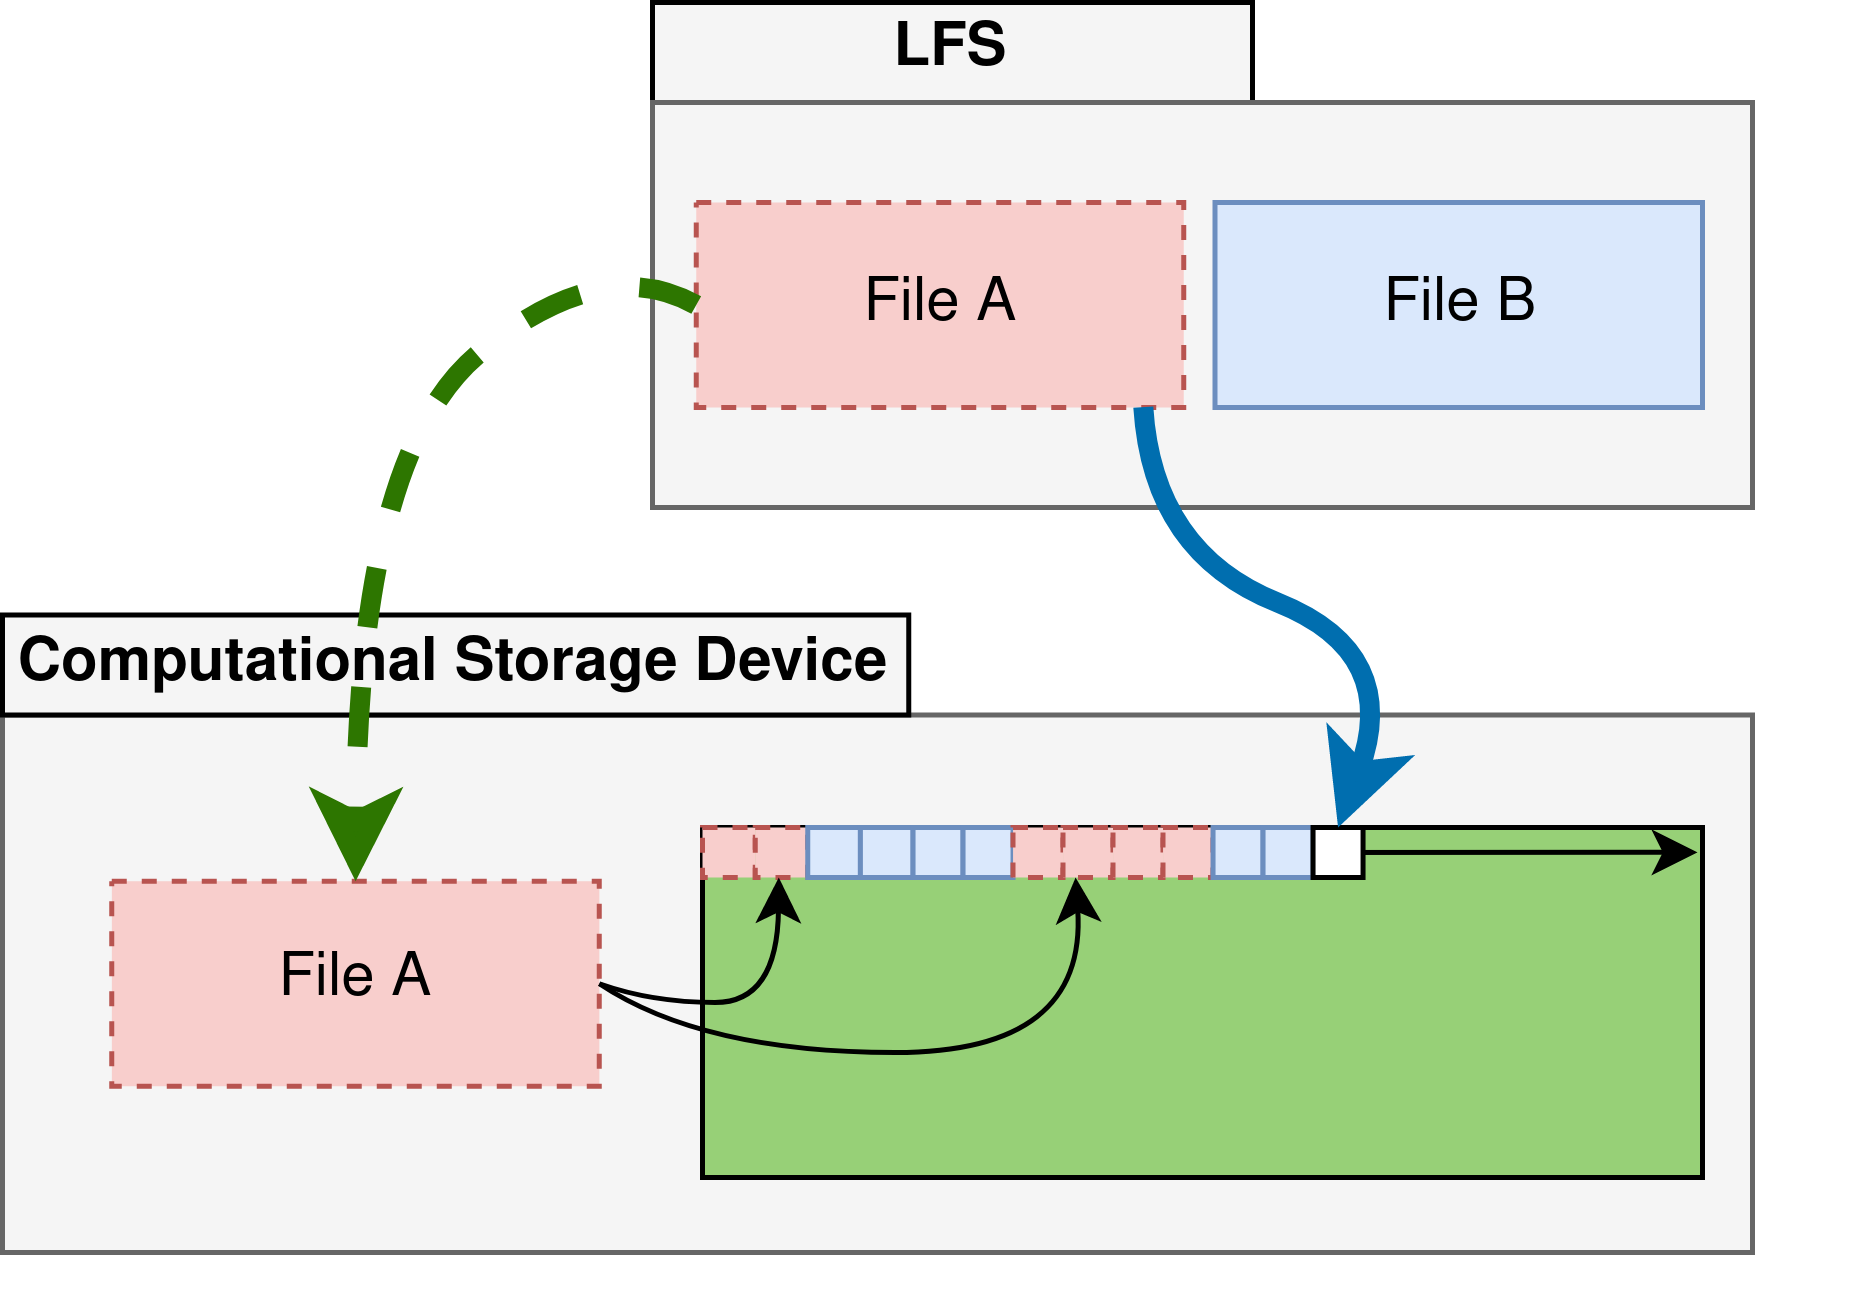
\includegraphics[width=0.9\linewidth]{resources/images/lfs.png}
		% \end{subfigure}
	\end{figure}
	\textit{\tiny $^{3}$F2FS: A New File System for Flash Storage}
	\endgroup
\end{frame}

% page 12
\begin{frame}{Implementation: Datastructures}
	\begingroup
	\small
	\begin{figure}[h]
		\centering
		% \begin{subfigure}{0.5\textwidth}
			%   \centering
			  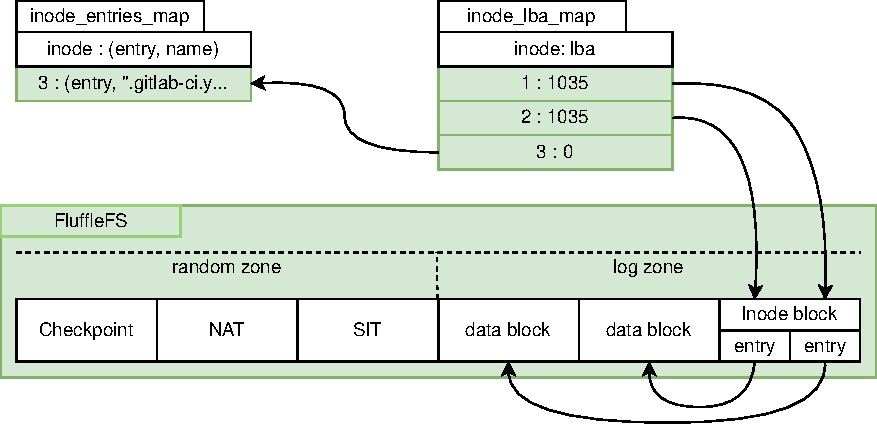
\includegraphics[width=1.0\linewidth]{resources/images/fluffle-inode-sync.pdf}
		% \end{subfigure}%
		% \begin{subfigure}{0.5\textwidth}
		% 	  \centering
		% 	  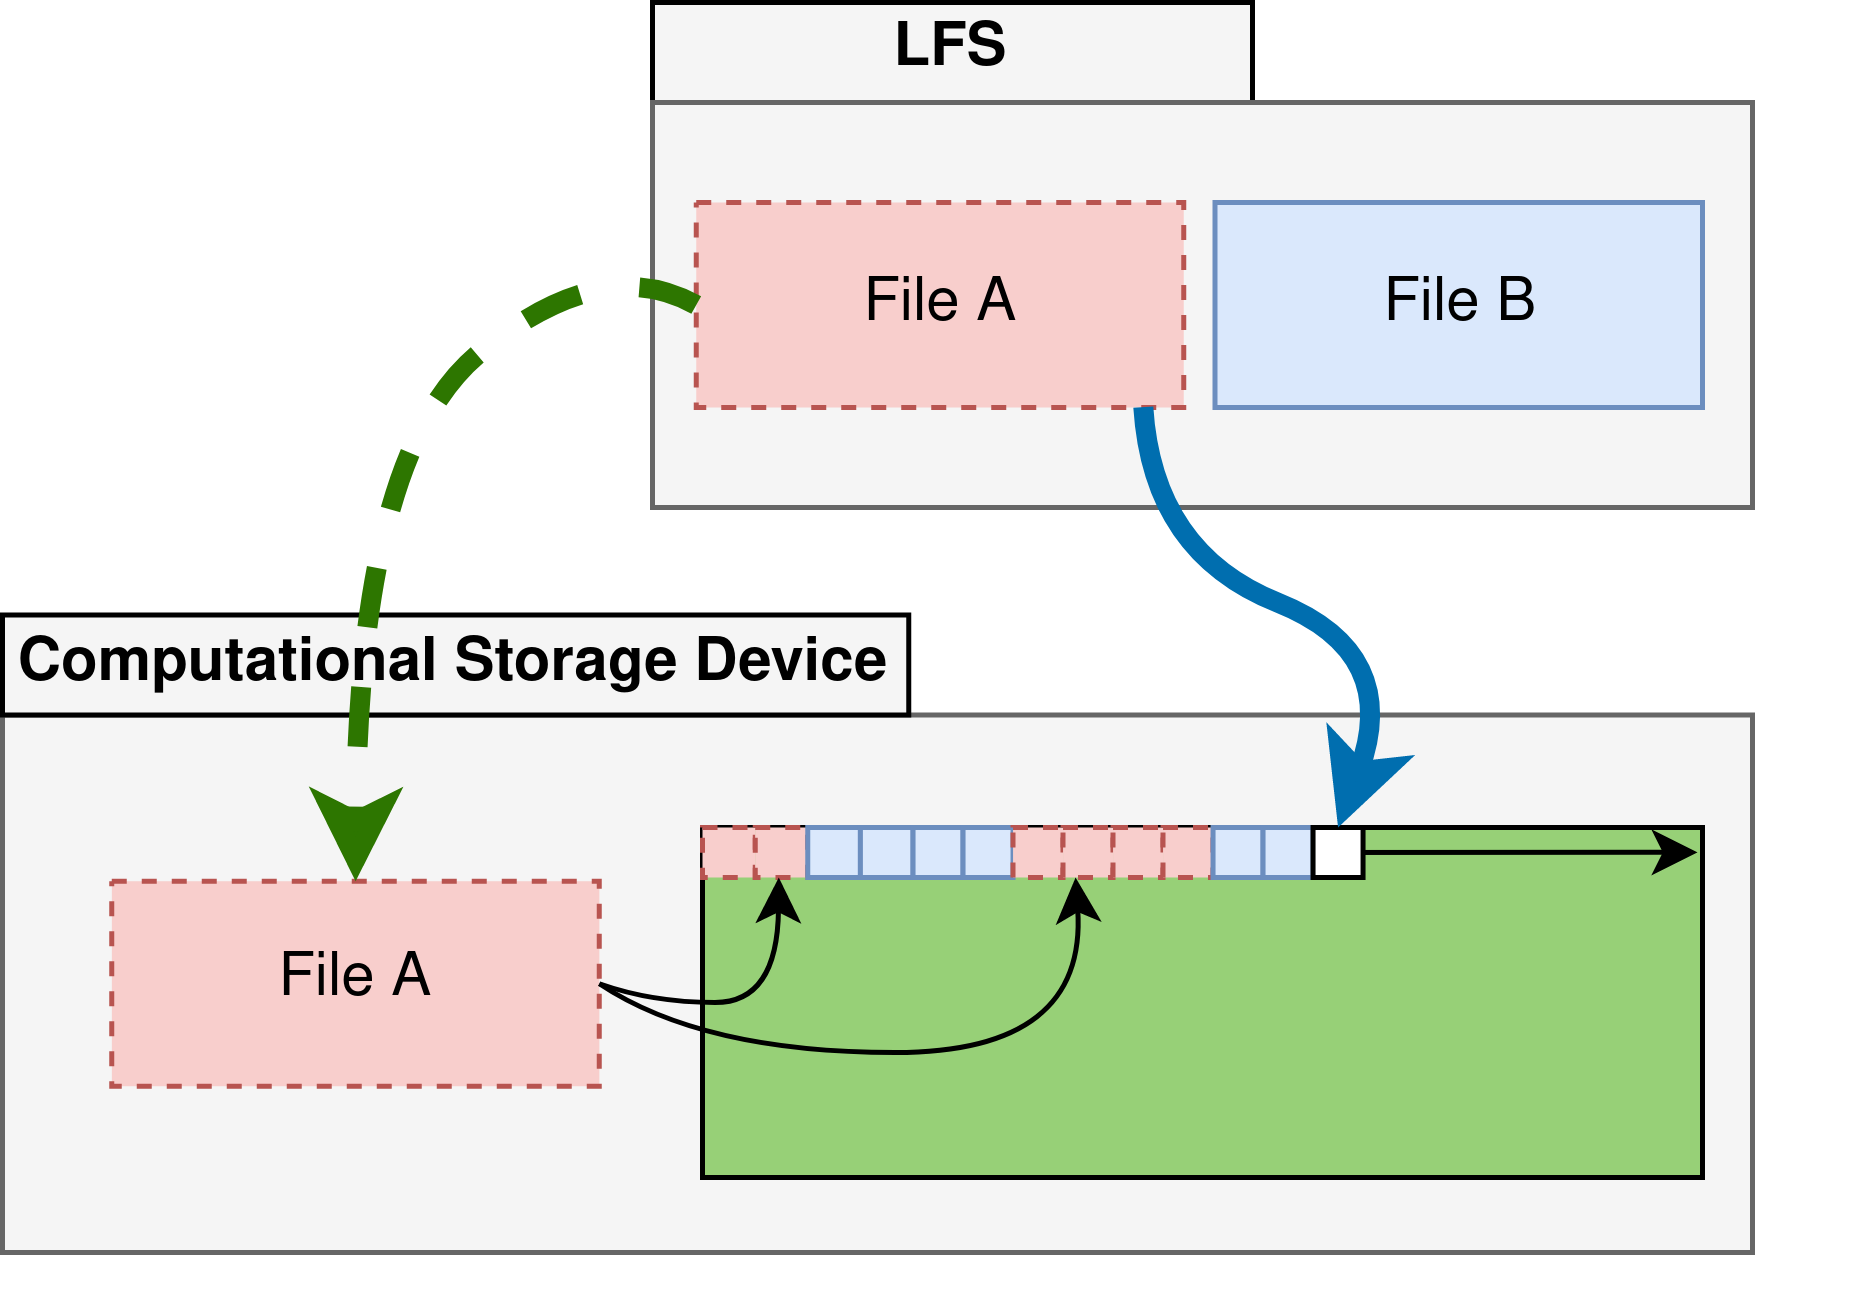
\includegraphics[width=0.9\linewidth]{resources/images/lfs.png}
		% \end{subfigure}
	\end{figure}
	\endgroup
\end{frame}

% page 10
% First is zoned namespaces. A ratified extensions to the NVMe specification
% the most prominent protocol used with Flash storage today. While the
% commercial availability of ZNS devices is still poor its benefits have already
% been prominently demonstrated in scientific literature. With zoned namespaces
% the host can no longer issue random writes as we have become used to from the
% traditional block interface. This means writes can no longer overwrite
% previously written data instead all writes are appended to the current write
% pointer separated across individual zones. This results in each zone being
% written sequentially. Should the host desire to erase data it must do so one
% entire zone at a time.
% \begin{frame}{Zoned NameSpaces (ZNS)}
% 	\begingroup
% 	\small
% 	\begin{figure}
% 		\centering
% 		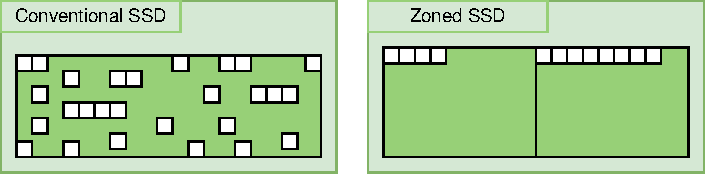
\includegraphics[width=1\textwidth]{resources/images/zns-vs-conventional-layout.pdf}
% 	\end{figure}
% 	\textit{\tiny $^{2}$NVM Express Zoned Namespace Command Set Specification 1.1b - 
% 	https://nvmexpress.org/developers/nvme-command-set-specifications/}
% 	\endgroup
% \end{frame}

% page 11
% We combine ZNS with a Log-structured File System,
% A filesystem design from the late 90's repopularized partly due to flash
% storage.
% LFS is Append-only, all writes go to the current tail of the log, even if the
% actual write overwrites parts of an already existing file. This allows to
% create in-memory representations of a file called snapshots that can be
% guaranteed to be immutable during the execution of a computational storage
% device program, often called kernels. Moreover this allows regular I/O 
% requests to happen concurrently even if the I/O goes to the same file.
% However, it does mean that the execution of the kernel can potentially operate
% on partially stale data.
% \begin{frame}{Log-structured File System (LFS)}
% 	\begingroup
% 	\small
% 	\begin{figure}
% 		\centering
% 		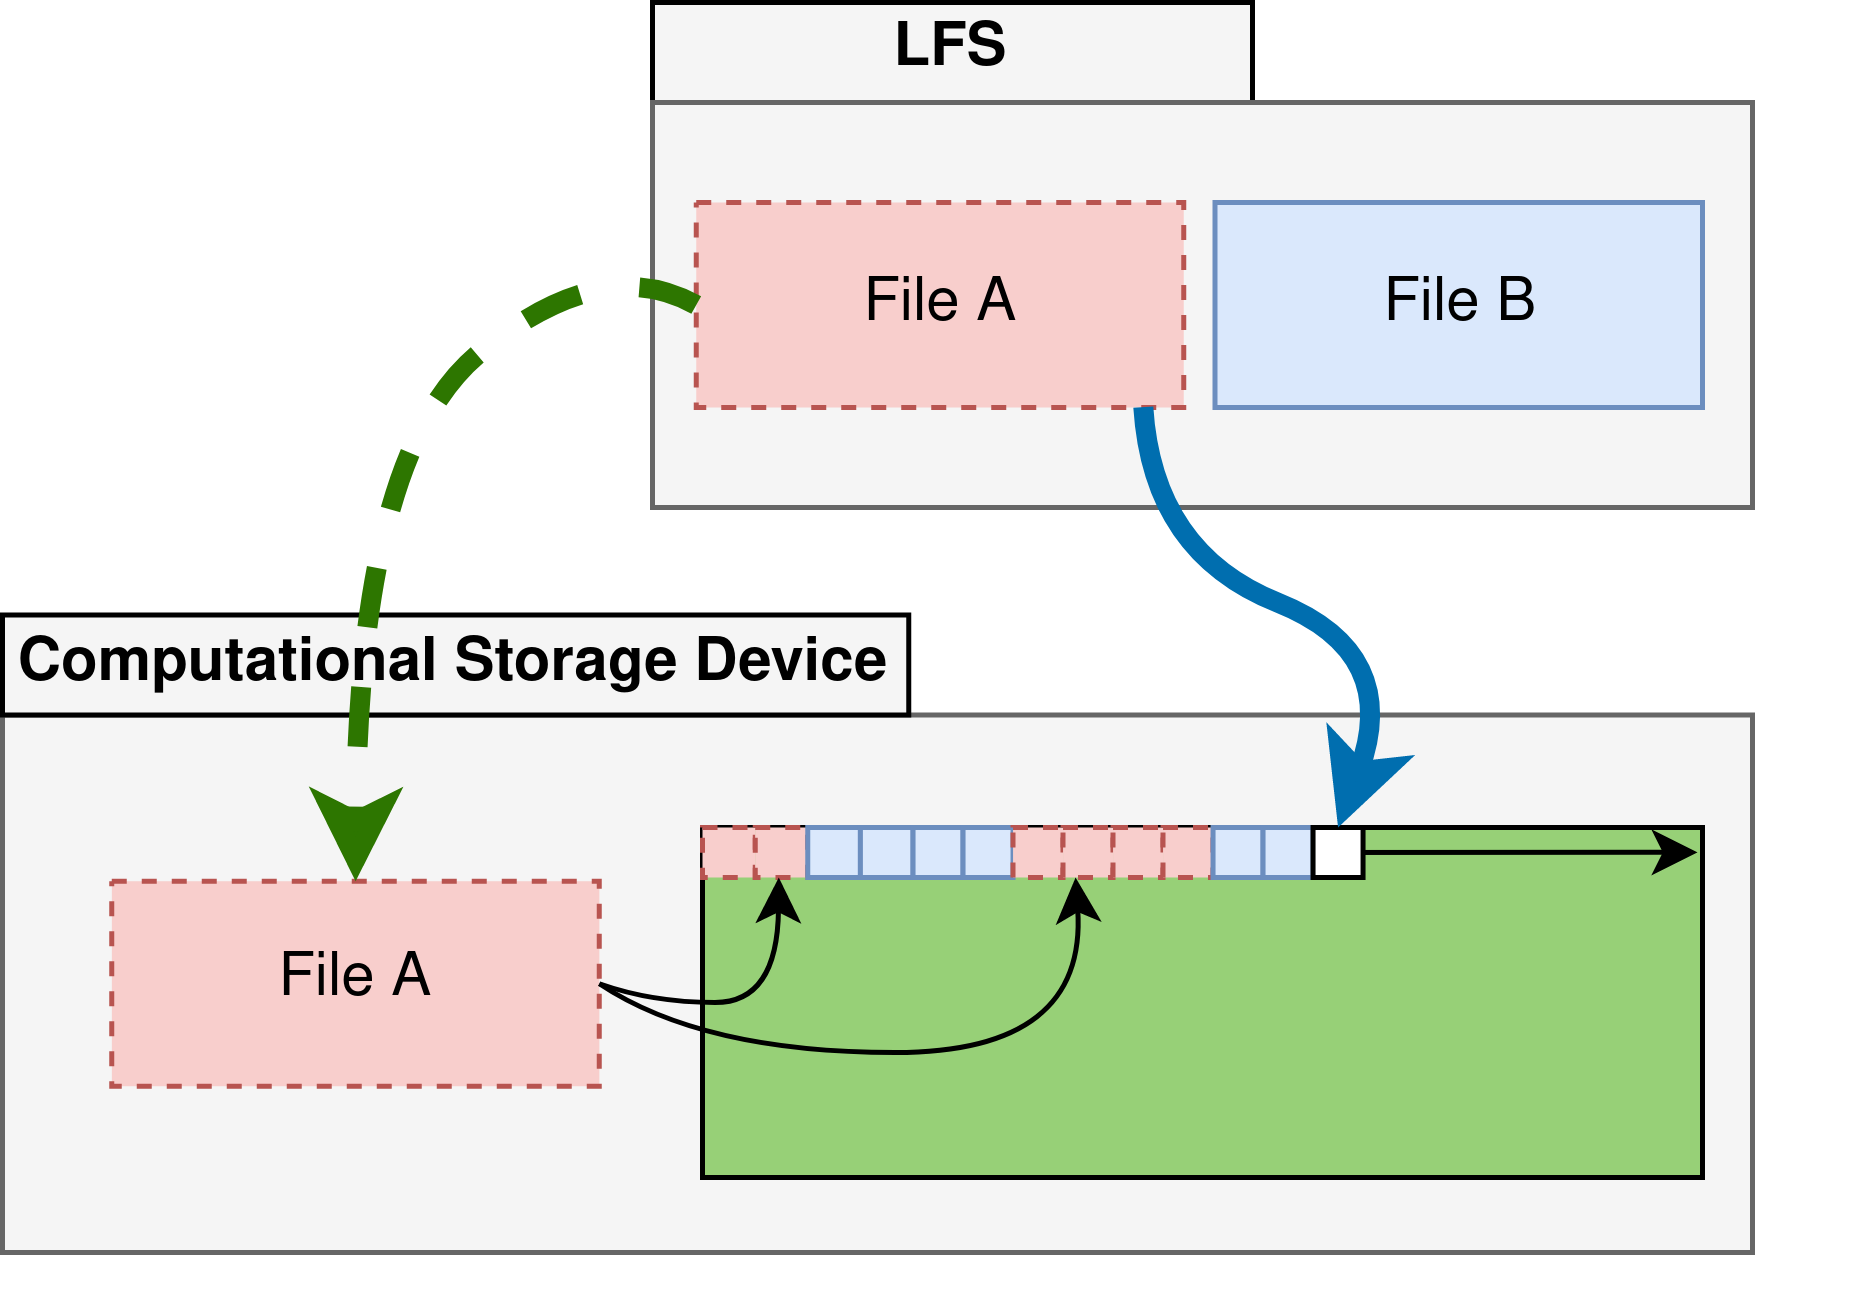
\includegraphics[width=0.7\textwidth]{resources/images/lfs.png}
% 	\end{figure}
% 	% \begin{itemize}
% 	% 	\item Append only writes
% 	% 	\item Journaling, snapshotting and revovery
% 	% 	\item Perfect match for ZNS
% 	% \end{itemize}
% 	% Append only writes
% 	% Simple support for journaling, snapshotting and revovery
% 	% Our design based on F2FS to prevent write-amplification
% 	% \begin{figure}
% 	% 	\centering
% 	% 	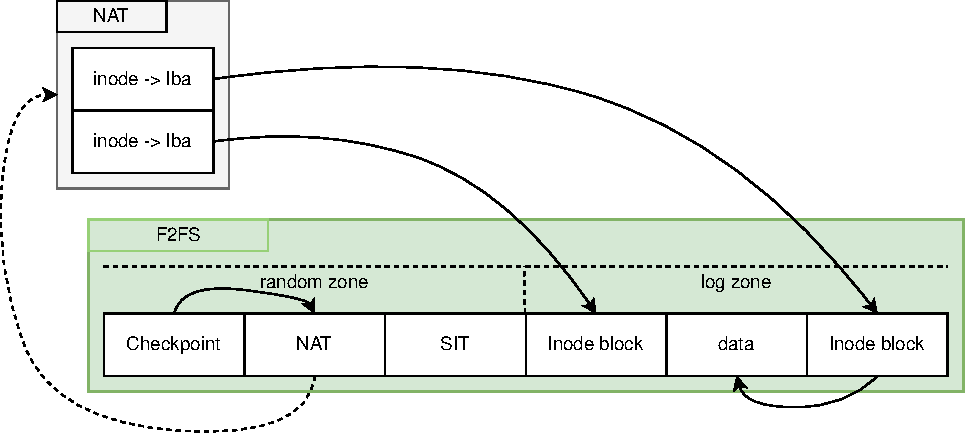
\includegraphics[width=0.7\textwidth]{resources/images/f2fs-nat.pdf}
% 	% \end{figure}
% 	\textit{\tiny $^{3}$The design and implementation of a Log-structured File System \\}
% 	\textit{\tiny $^{4}$F2FS: A New File System for Flash Storage}
% 	\endgroup
% \end{frame}

% page 12
% \begin{frame}{extended Berkely Packet Filter (eBPF)}
% 	\begingroup
% 	\small
% 	% used in the Linux kernel but effectively its an ISA like x86 but easy
% 	% to implement in virtual machines
% 	\begin{figure}
% 		\centering
% 		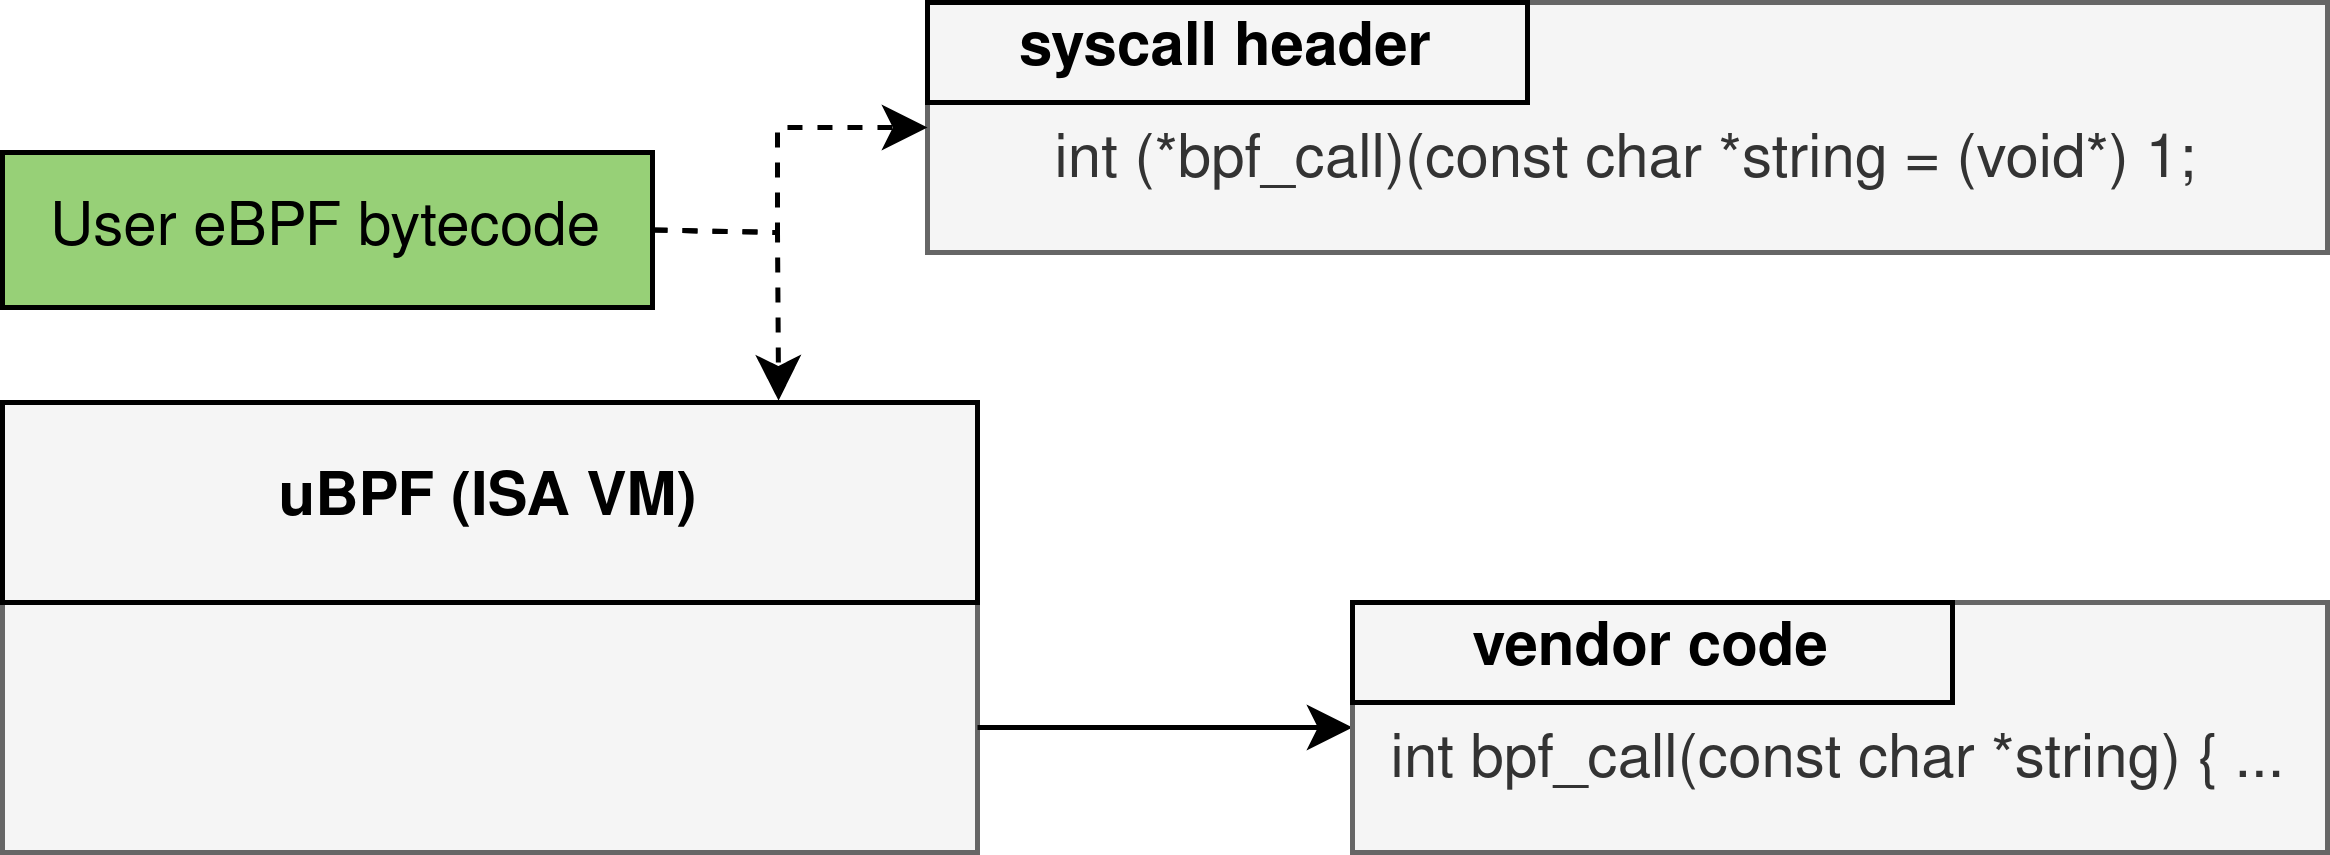
\includegraphics[width=1\textwidth]{resources/images/ubpf-simple.png}
% 	 \end{figure}
% 	\endgroup
% \end{frame}

% page 13
% With these technologies it is clear how we can support multi-user tenent
% file system access in a computational storage device setting. We now
% demonstrate the exact mechanism of registering and offloading programs as used
% in FluffleFS. First is the compilation process of the kernel by the end user.
% This is done through two header files one for CSD operations itself such as
% reading from the storage device and returning data to the host. The other
% specific to the FluffleFS filesystem. It should be noted that the CSD header
% is already written in a manor that allows for vendor agnostic implementation.
% Meaning that this header prevents users from having to recompile their kernels
% for different CSD vendors. Designing an file system agnostic interface
% remains an open research question, however.
% \begin{frame}{FluffleFS}
% 	\begingroup
% 	\small % FUSE LFS with concurrent regular and CSD access even to the same file.
% 	\begin{figure}
% 		\centering
% 		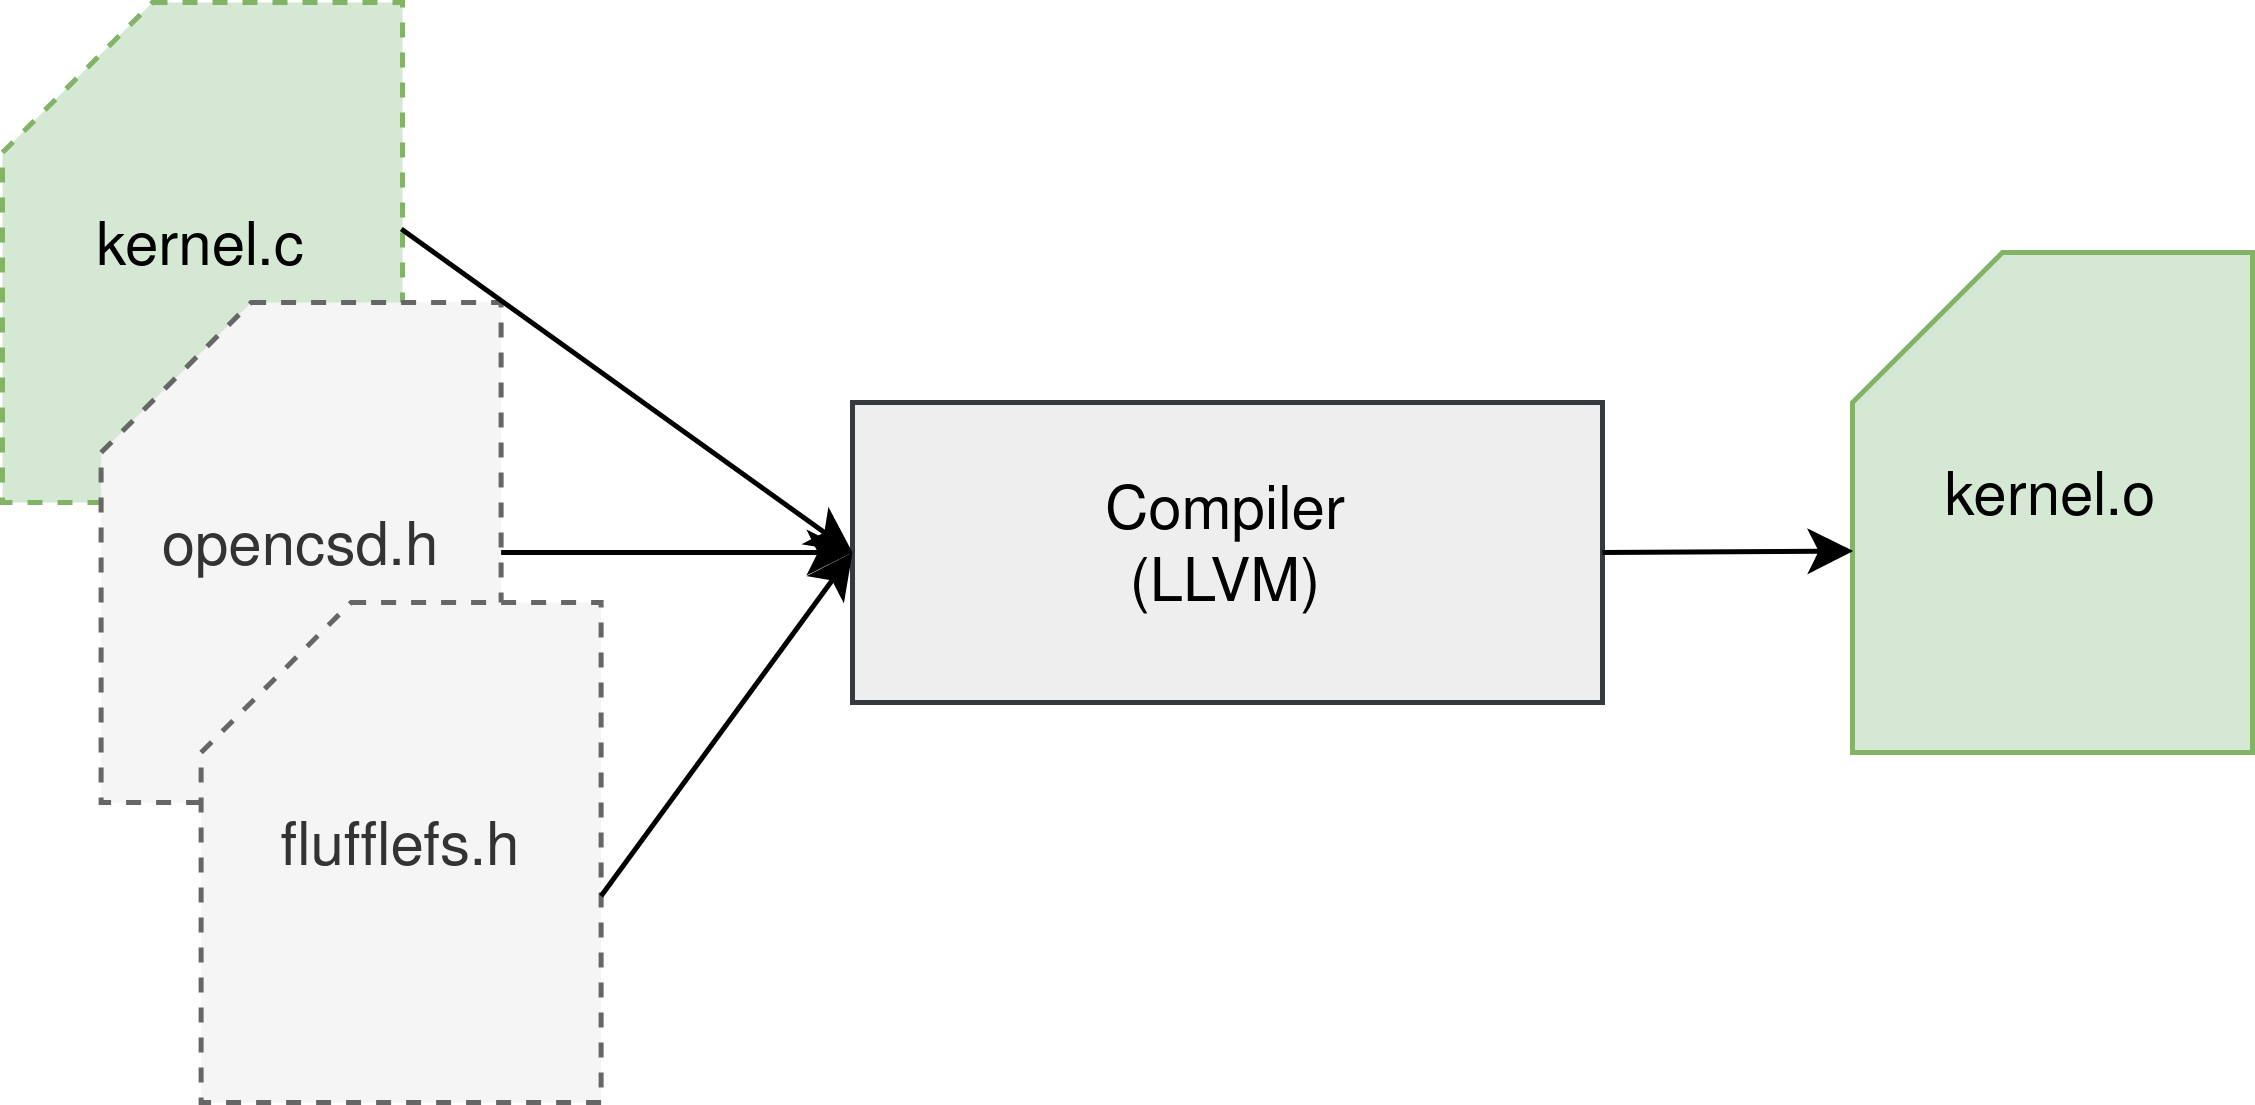
\includegraphics[width=0.7\textwidth]{resources/images/compile.png}
% 	\end{figure}
% 	% How does FluffleFS combine these technologies
% 	% \begin{itemize}
% 	% 	\item Why ZNS, LFS \& eBPF?
% 	% 	\item CSD kernels operate on snapshots % concurrent regular and offloaded access even on the same file
% 	% 	\item PID + inode pairs for xattr state % in memory only
% 	% \end{itemize}
% 	\endgroup
% \end{frame}

% page 13
% Now I imagine this particular diagram can seem daunting but lets go through
% it step by step. First are the bold arrows with underlined word, each word
% represents a specific system call that is implemented by POSIX complaint
% operating systems and Windows. First, the user program issues the stat call on
% the compiled kernel file, this provides an inode number which is temporarily
% stored in a key value pair as shown in the top left. Second, the user
% issues an open on the file that is going to be offloaded to the CSD. Third,
% and this is key, the user calls set extended attribute on the offloaded file,
% configuring a specific key value pair that indicates to the filesystem that
% this offloading should occur. As soon as this extended attribute is set, the
% file system snapshots both the kernel and target file and moves their in-memory
% representations onto the CSD. Lastly, the user issues a read command on the
% file, this bypasses the host filesystem and instead a process is spawned on
% the CSD. The CSD process runs the snapshotted kernel operating on the
% snapshotted file. In the end the results of the kernel are returned to the
% user as if it was the data that was read from the file. And this is how we
% achieve CSD offloading without any changes to existing operating systems APIs.
% No changes, to existing operating systems are necessary to achieve this
% process in this way.
\begin{frame}{Implementation: Offloading}
	\begingroup
	\small % FUSE LFS with concurrent regular and CSD access even to the same file.
	\begin{figure}
		\centering
		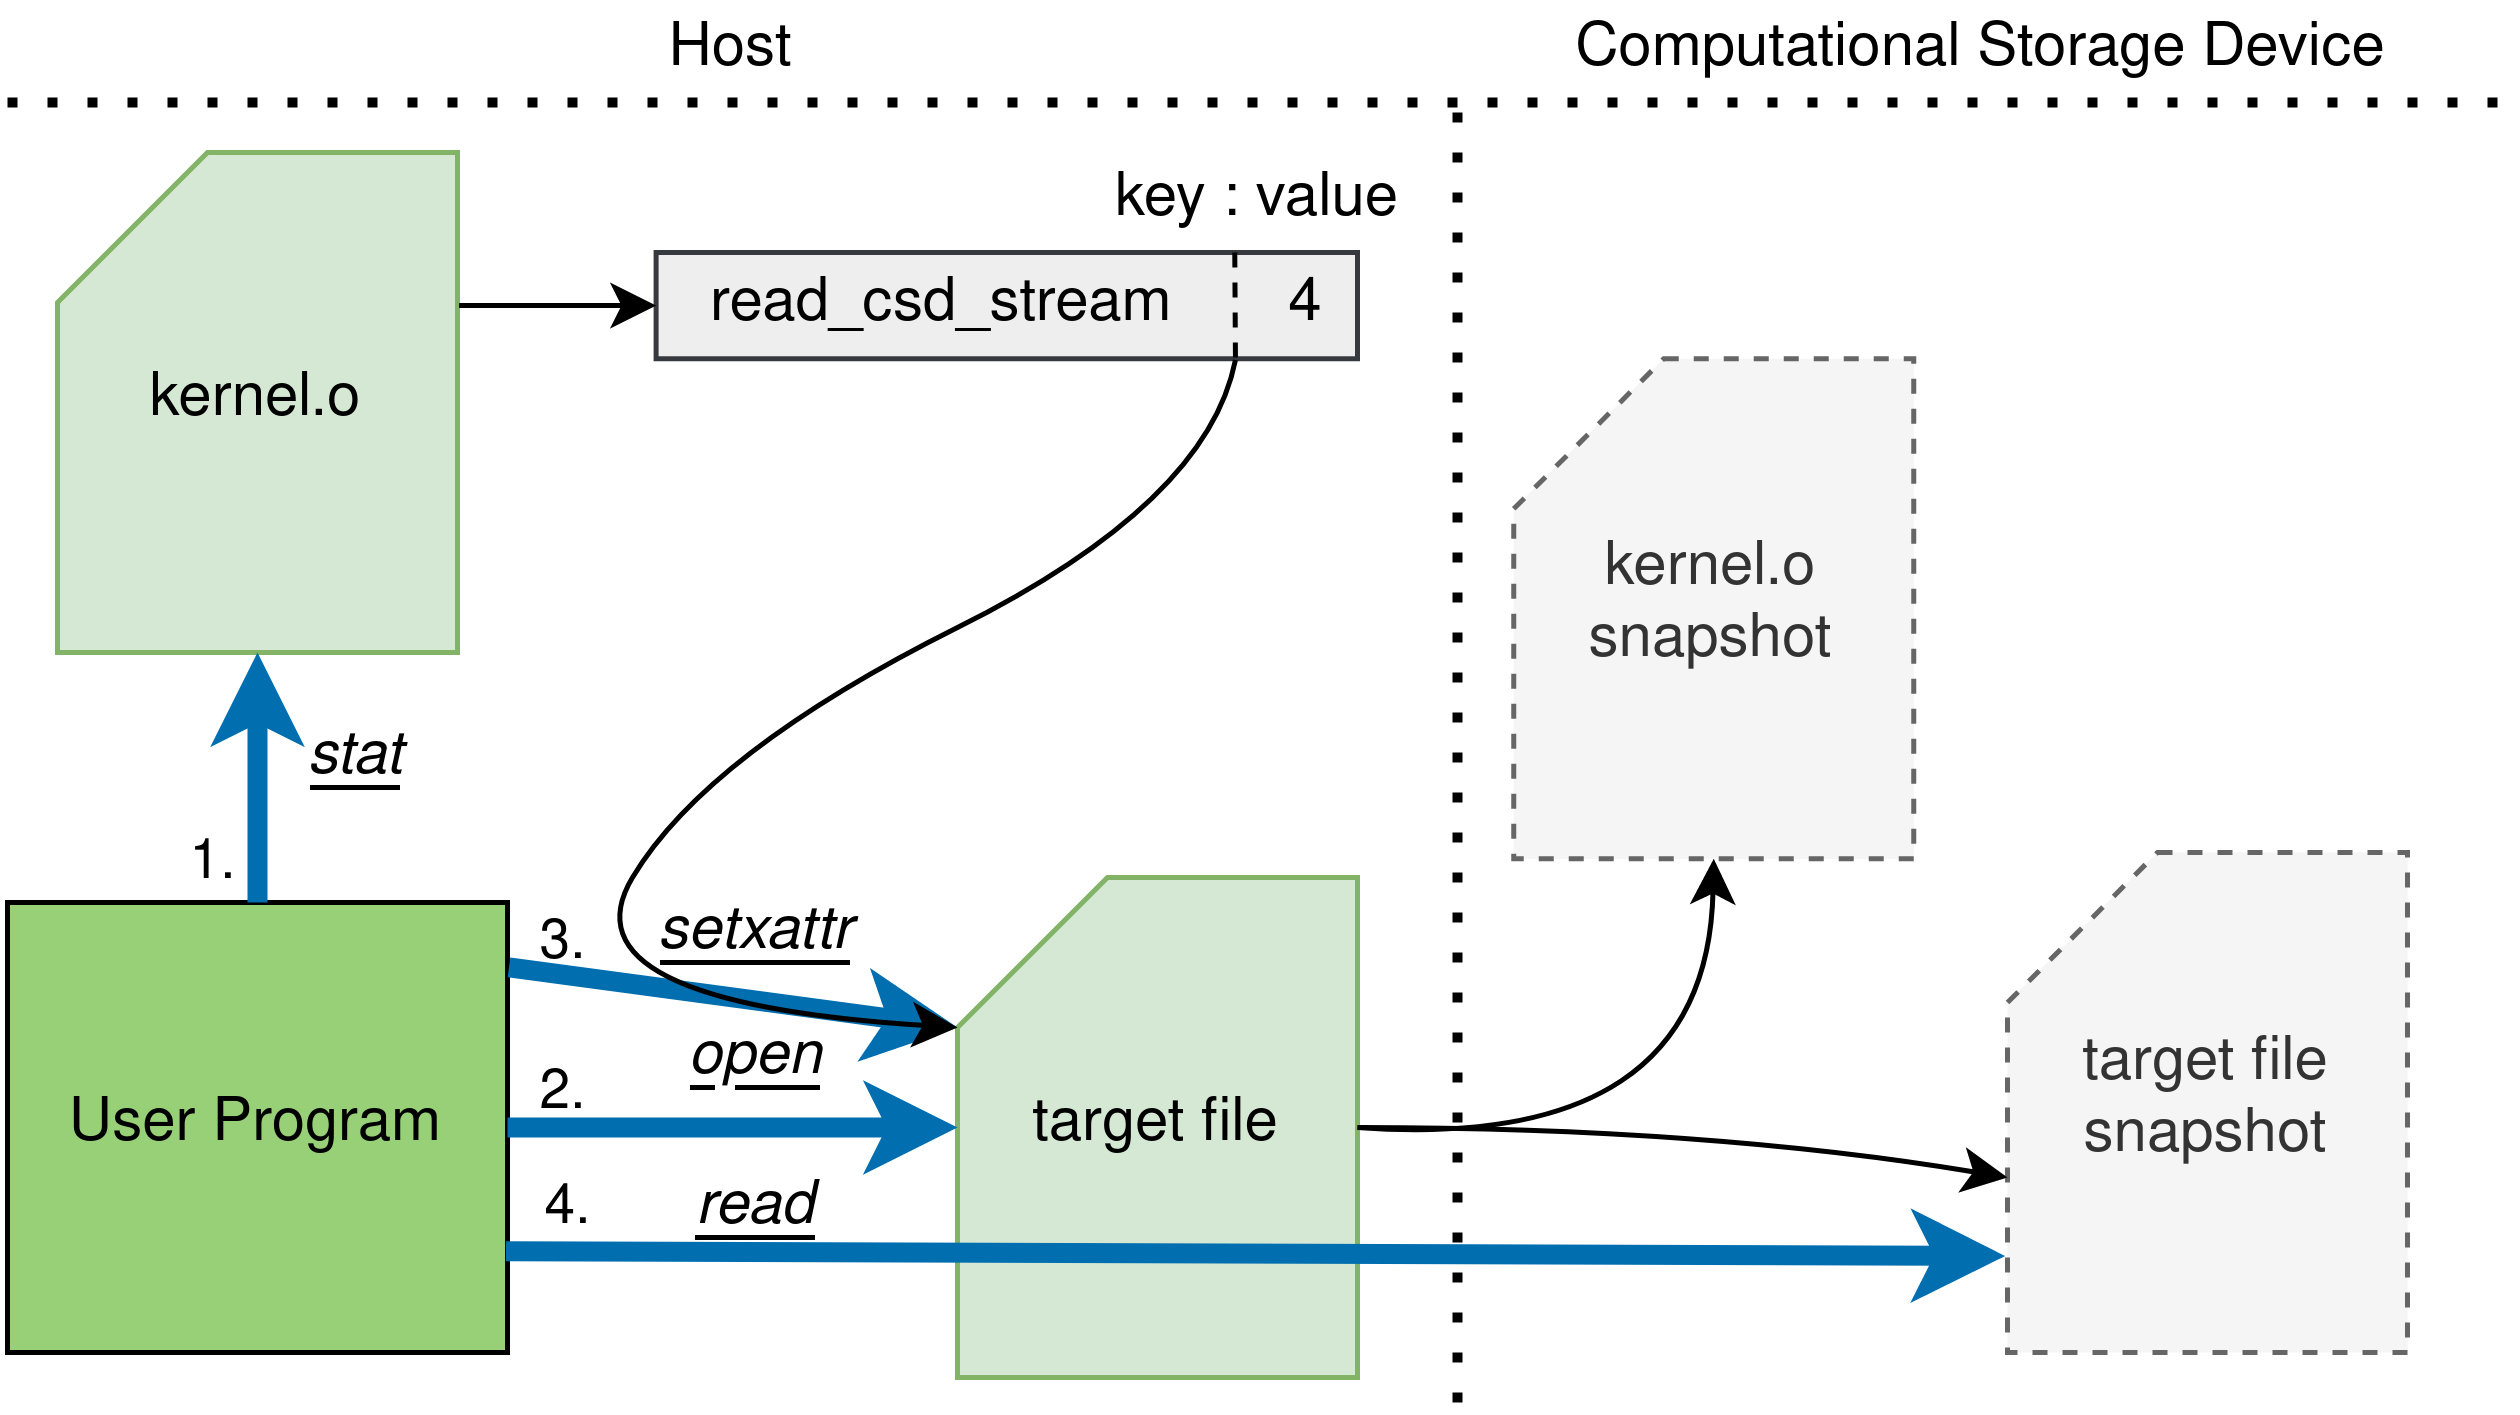
\includegraphics[width=0.9\textwidth]{resources/images/offloading.png}
	\end{figure}
	% How does FluffleFS combine these technologies
	% \begin{itemize}
	% 	\item Why ZNS, LFS \& eBPF?
	% 	\item CSD kernels operate on snapshots % concurrent regular and offloaded access even on the same file
	% 	\item PID + inode pairs for xattr state % in memory only
	% \end{itemize}
	\endgroup
\end{frame}

% page 14
\begin{frame}{Implementation: Offloading}
	\begingroup
	\small % FUSE LFS with concurrent regular and CSD access even to the same file.
	\begin{figure}
		\centering
		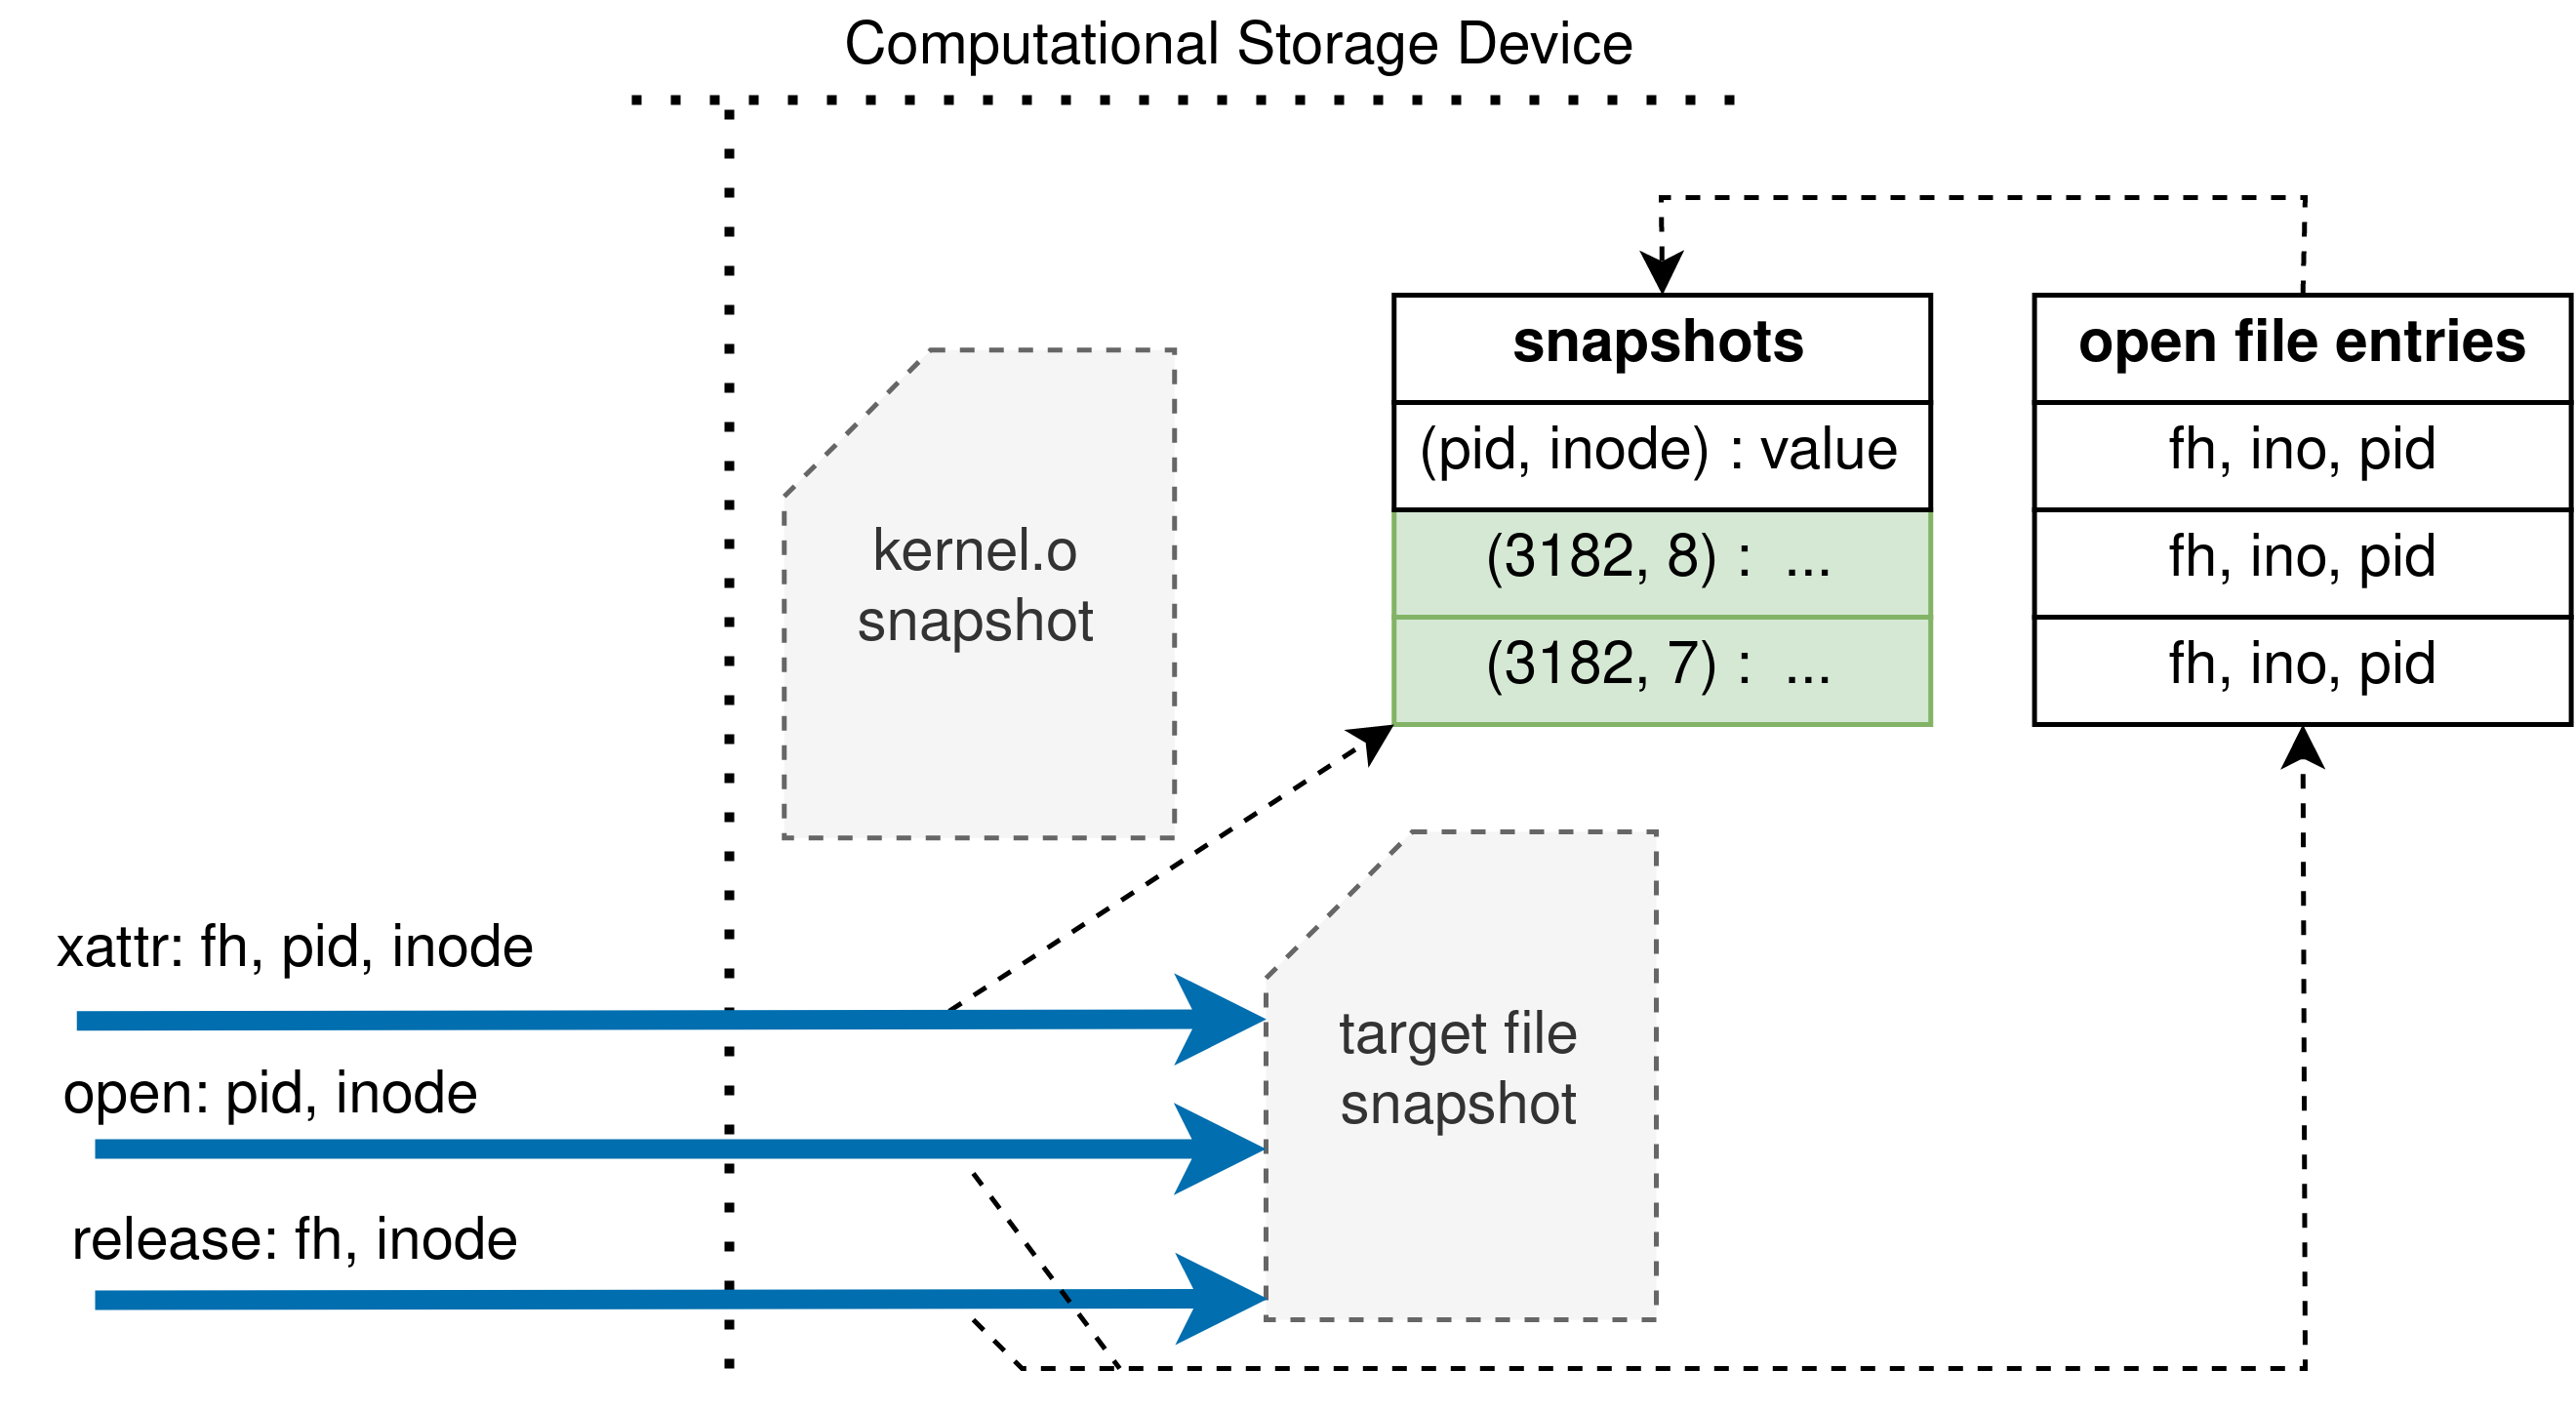
\includegraphics[width=0.9\textwidth]{resources/images/offloading-management.png}
	\end{figure}
	% How does FluffleFS combine these technologies
	% \begin{itemize}
	% 	\item Why ZNS, LFS \& eBPF?
	% 	\item CSD kernels operate on snapshots % concurrent regular and offloaded access even on the same file
	% 	\item PID + inode pairs for xattr state % in memory only
	% \end{itemize}
	\endgroup
\end{frame}

% page 15
\begin{frame}{Evaluation: Setup}
	\begingroup
	\tiny iodepth 1, single file throughput, min / max error bars.
	
	\endgroup
\end{frame}

% page 16
\begin{frame}{Evaluation: Sequential Performance}
	\begingroup
	\begin{figure}
		\begin{subfigure}{0.5\textwidth}
			\centering
			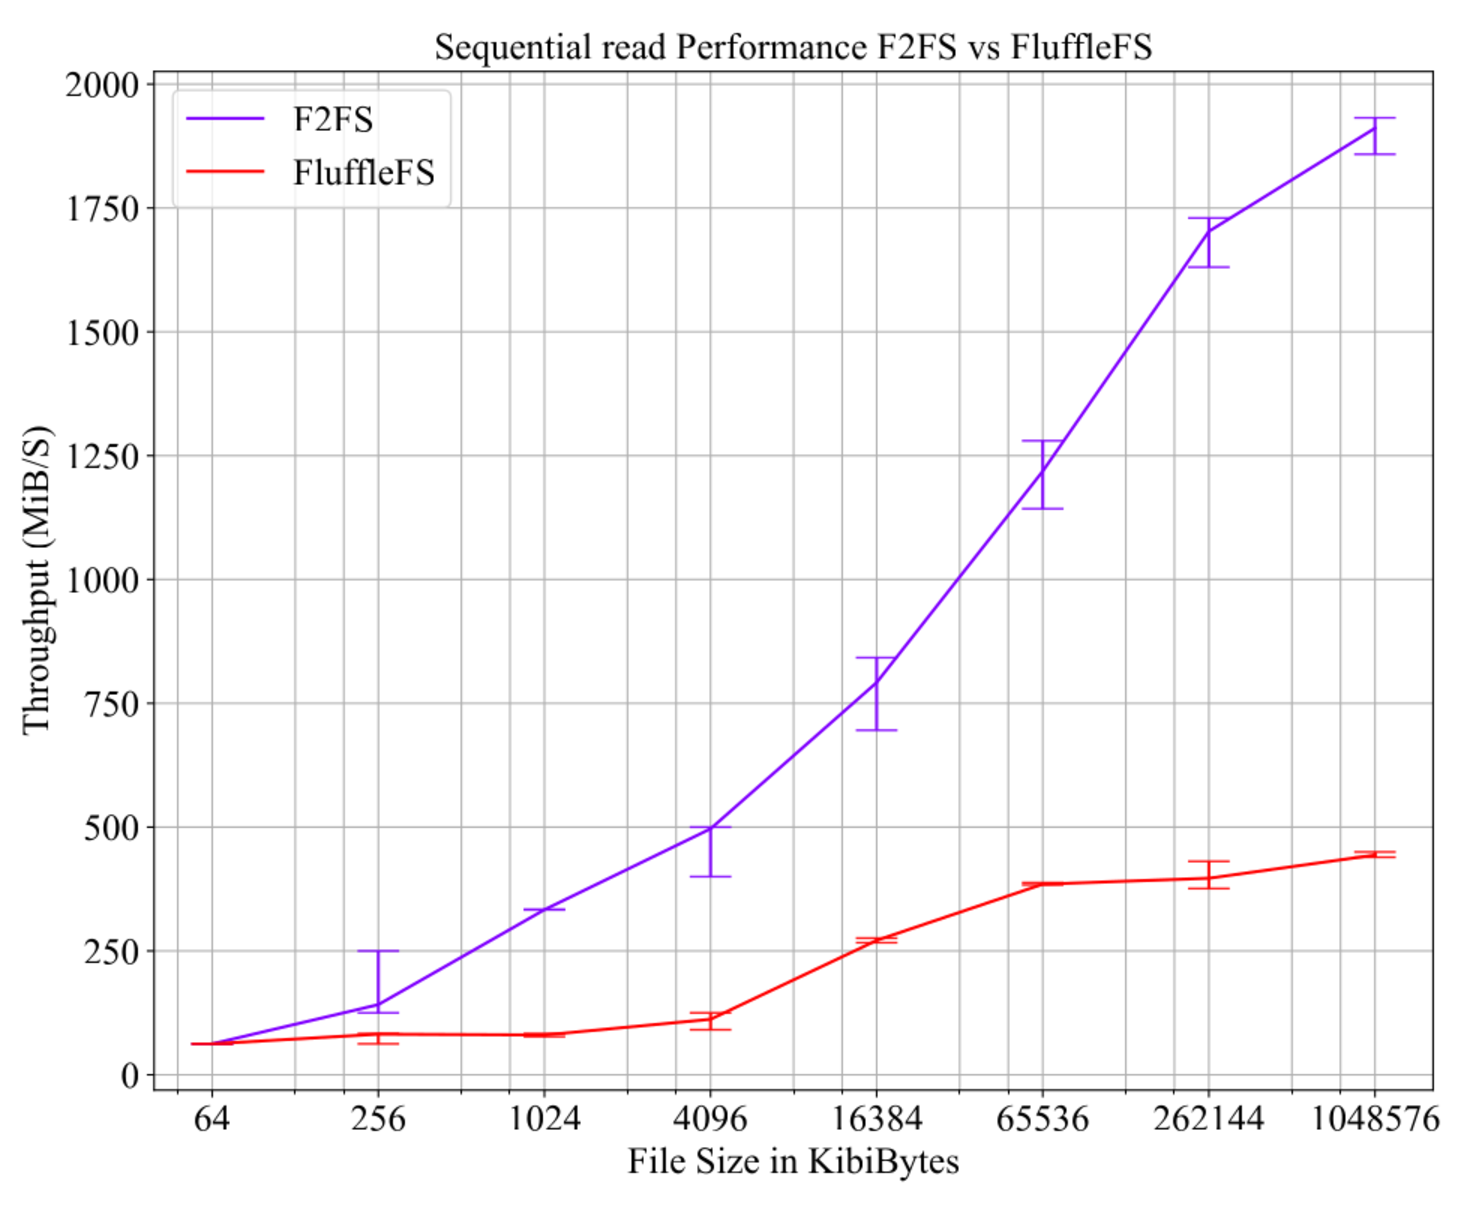
\includegraphics[width=1.0\linewidth]{resources/images/results-sequential.pdf}
		\end{subfigure}%
		\begin{subfigure}{0.5\textwidth}
			\centering
			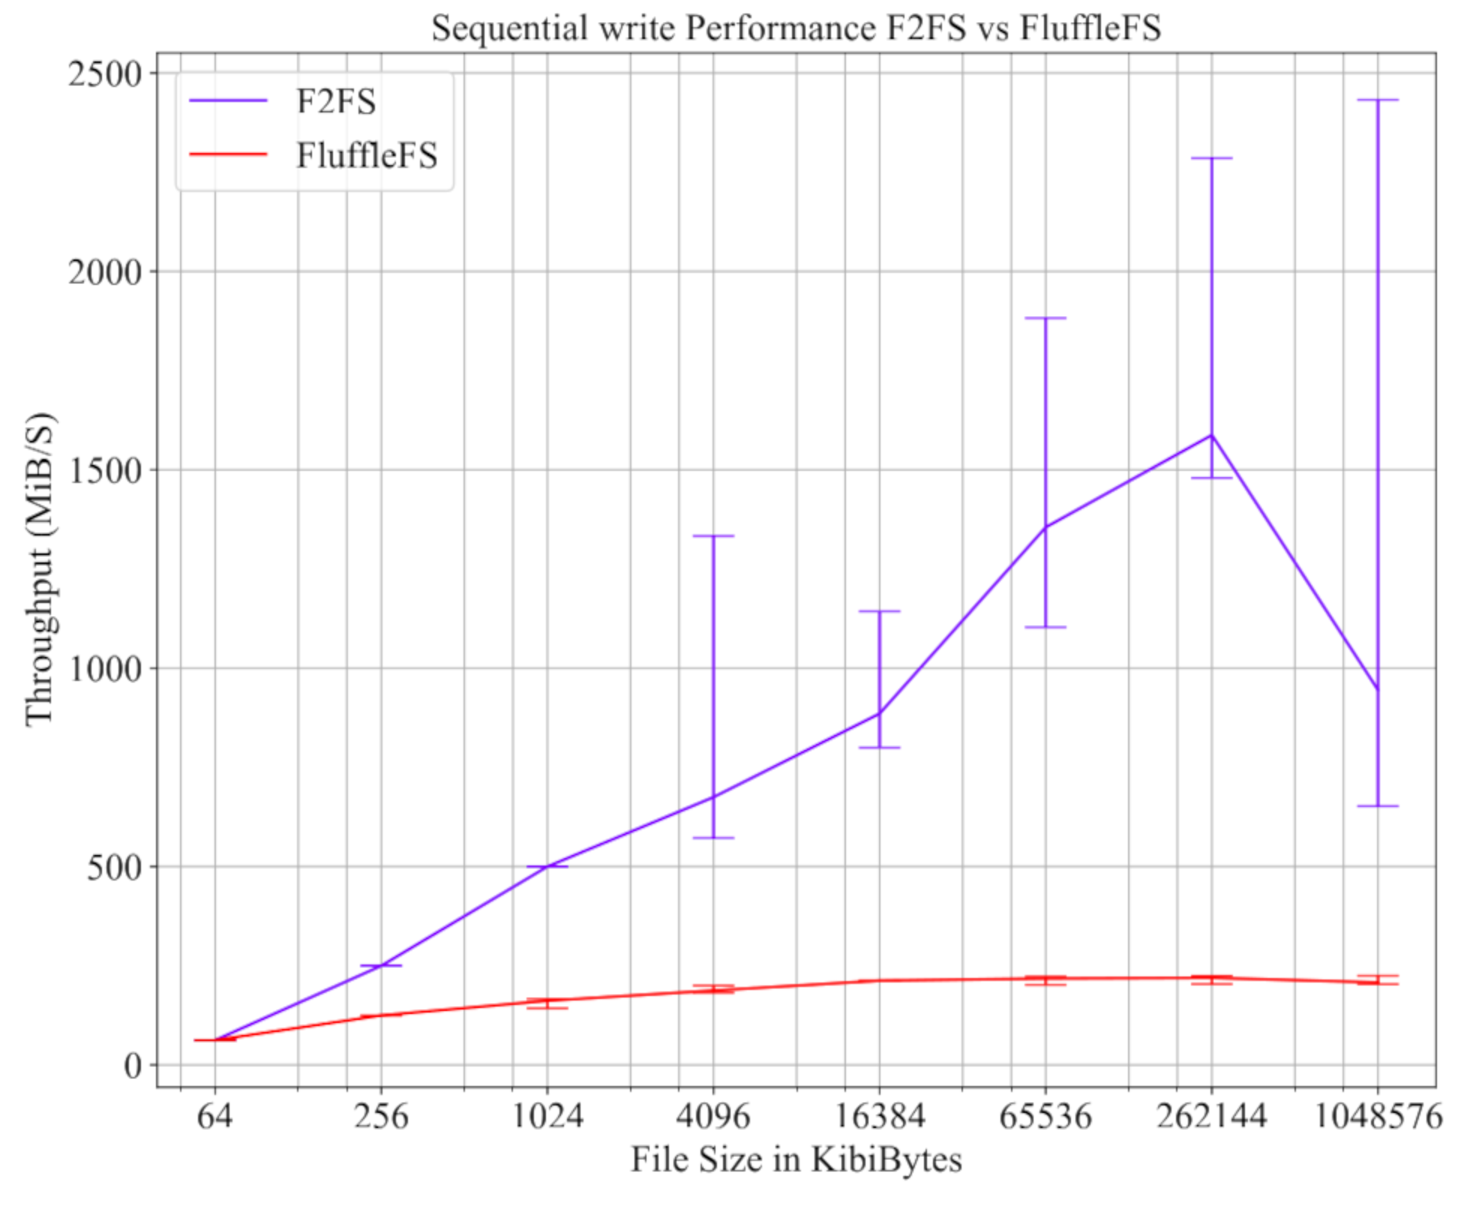
\includegraphics[width=1.0\linewidth]{resources/images/results-sequential-write.pdf}
		\end{subfigure}
	\end{figure}
	\tiny iodepth 1, single file throughput, min / max error bars.
	\endgroup
\end{frame}

% page 17
\begin{frame}{Evaluation: Kernel Passthrough}
	\begingroup
	% \small An emulated programmable computational flash storage device
	\begin{figure}
		\centering
		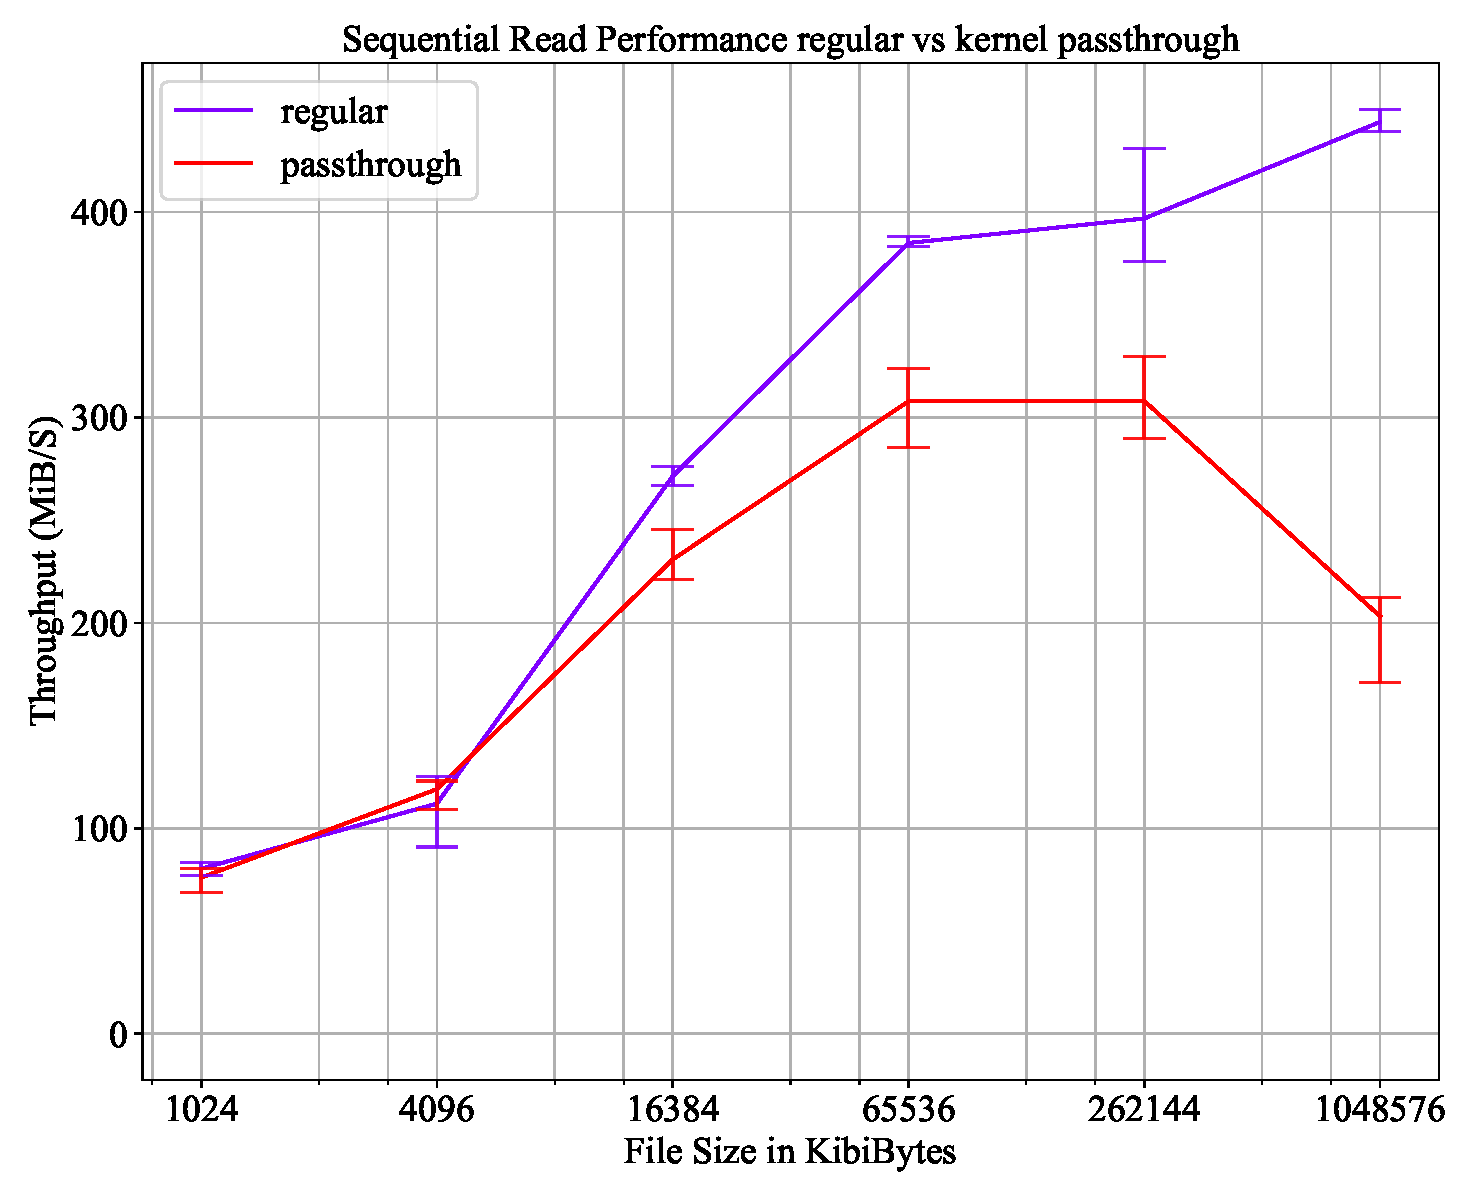
\includegraphics[width=0.65\textwidth]{resources/images/results-passthrough.pdf}
	\end{figure}
	\tiny What is the performance overhead of offloading for max throughput?
	\endgroup
\end{frame}

% page 18
% Knowing how offloading is achieved we can now turn to a practical example.
% Background compression algorithms often check if a file is fit for compression
% prior to compressing it. This is done by computing the shannon entropy across
% the first portion of a file, in our case 512k. The shannon entropy is measured
% as a single 32 bits float with a value between 0 and 8. 8 being entirely 
% incompressable and 0 meaning compressable to 0 size. We perform this
% computation for 32 individual files with both the computation performed by the
% host and offloaded. With the offloaded application almost the entire spent is
% waiting for the result of the kernel. During this time the operating system
% can schedule other processes to use the CPU instead. This means that for this
% application the host load is signifcantly reduced. Since such a compression
% task runs in the background it would be acceptable if the total execution time
% would be longer, however, this is not the case in our results.
\begin{frame}{Evaluation: Background Compression}
	\begingroup
	% \small An emulated programmable computational flash storage device
	\begin{figure}
		\begin{subfigure}{0.5\textwidth}
			\centering
			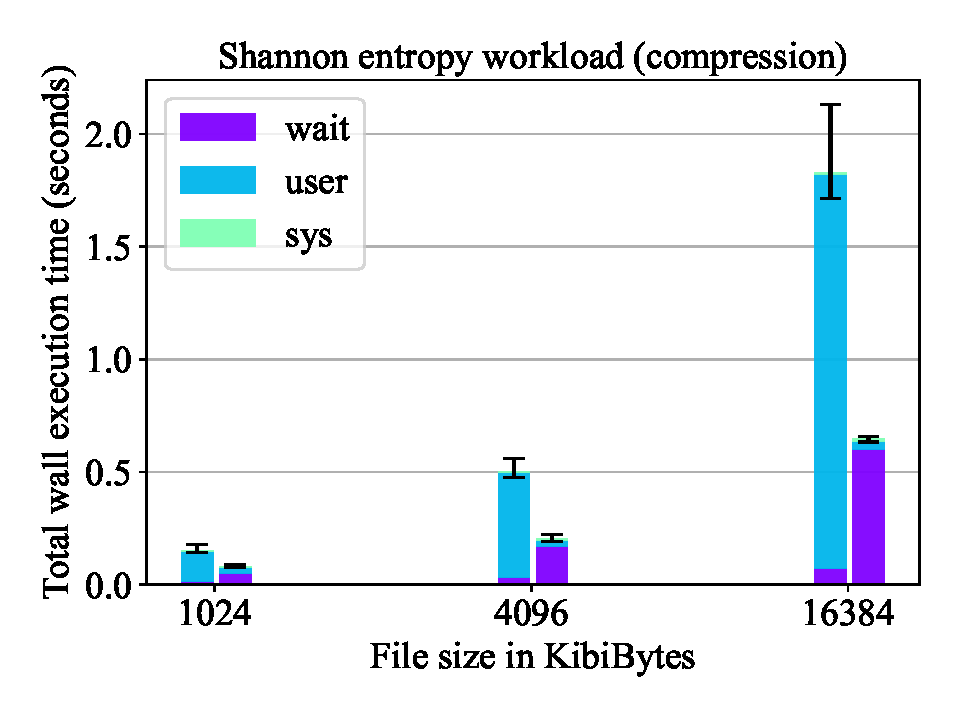
\includegraphics[width=1.0\linewidth]{resources/images/results-shannon-lower.pdf}
		\end{subfigure}%
		\begin{subfigure}{0.5\textwidth}
			\centering
			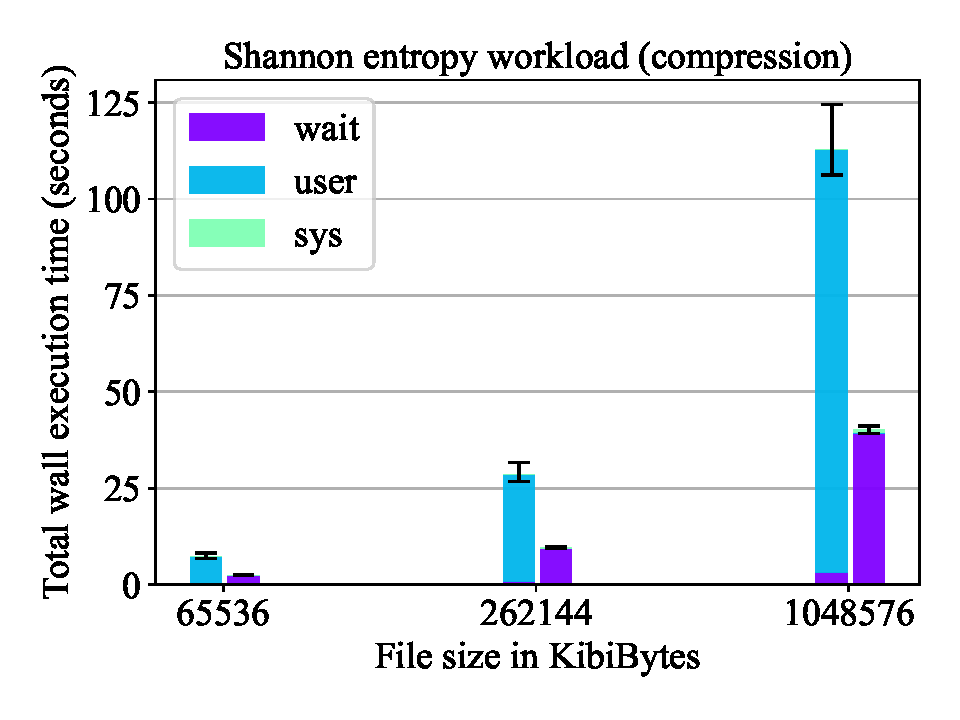
\includegraphics[width=1.0\linewidth]{resources/images/results-shannon-upper.pdf}
		\end{subfigure}
	\end{figure}
	\tiny Split for small and big files, different time scales (y axis)
	% \begin{figure}
	% 	\centering
	% 	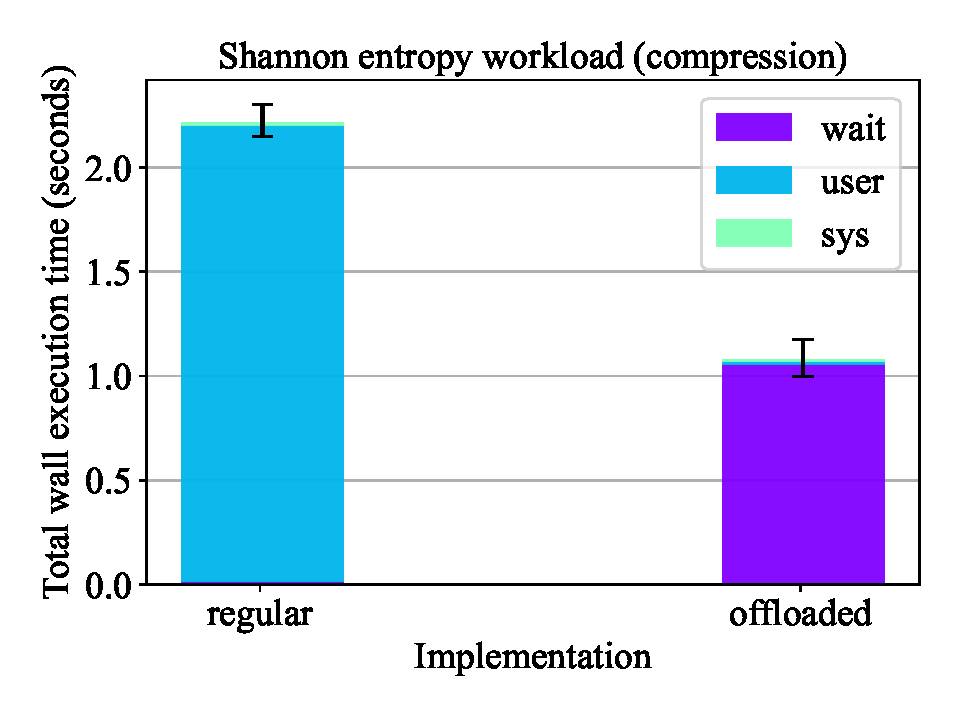
\includegraphics[width=0.8\textwidth]{resources/images/results.pdf}
	% \end{figure}
	\endgroup
\end{frame}

% page 16
% \begin{frame}{Evaluation Application}
% 	\begingroup
% 	% \small An emulated programmable computational flash storage device
% 	% \begin{figure}
% 	% 	\centering
% 	% 	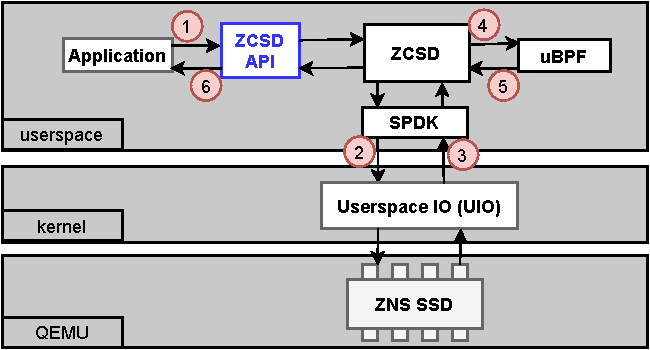
\includegraphics[width=0.8\textwidth]{resources/images/zcsd-arch-final}
% 	% \end{figure}
% 	\endgroup
% \end{frame}

% page 17
% \begin{frame}{In short}
% 	\begingroup
% 	\small OpenCSD \& FluffleFS demonstrate a filesystem design that allows for
% 	multi-user tenant CSDs agnostic to vendor SSD implementations.
% 	\endgroup
% \end{frame}

% page 18
% \begin{frame}{Future Work}
% 	\begingroup
% 	\small
% 	\begin{itemize}
% 		\item File system agnostic integration for CSDs
% 		\item Static analysis \& security
% 		\item Endianness conversions
% 	\end{itemize}
% 	% \begin{figure}
% 	% 	\centering
% 	% 	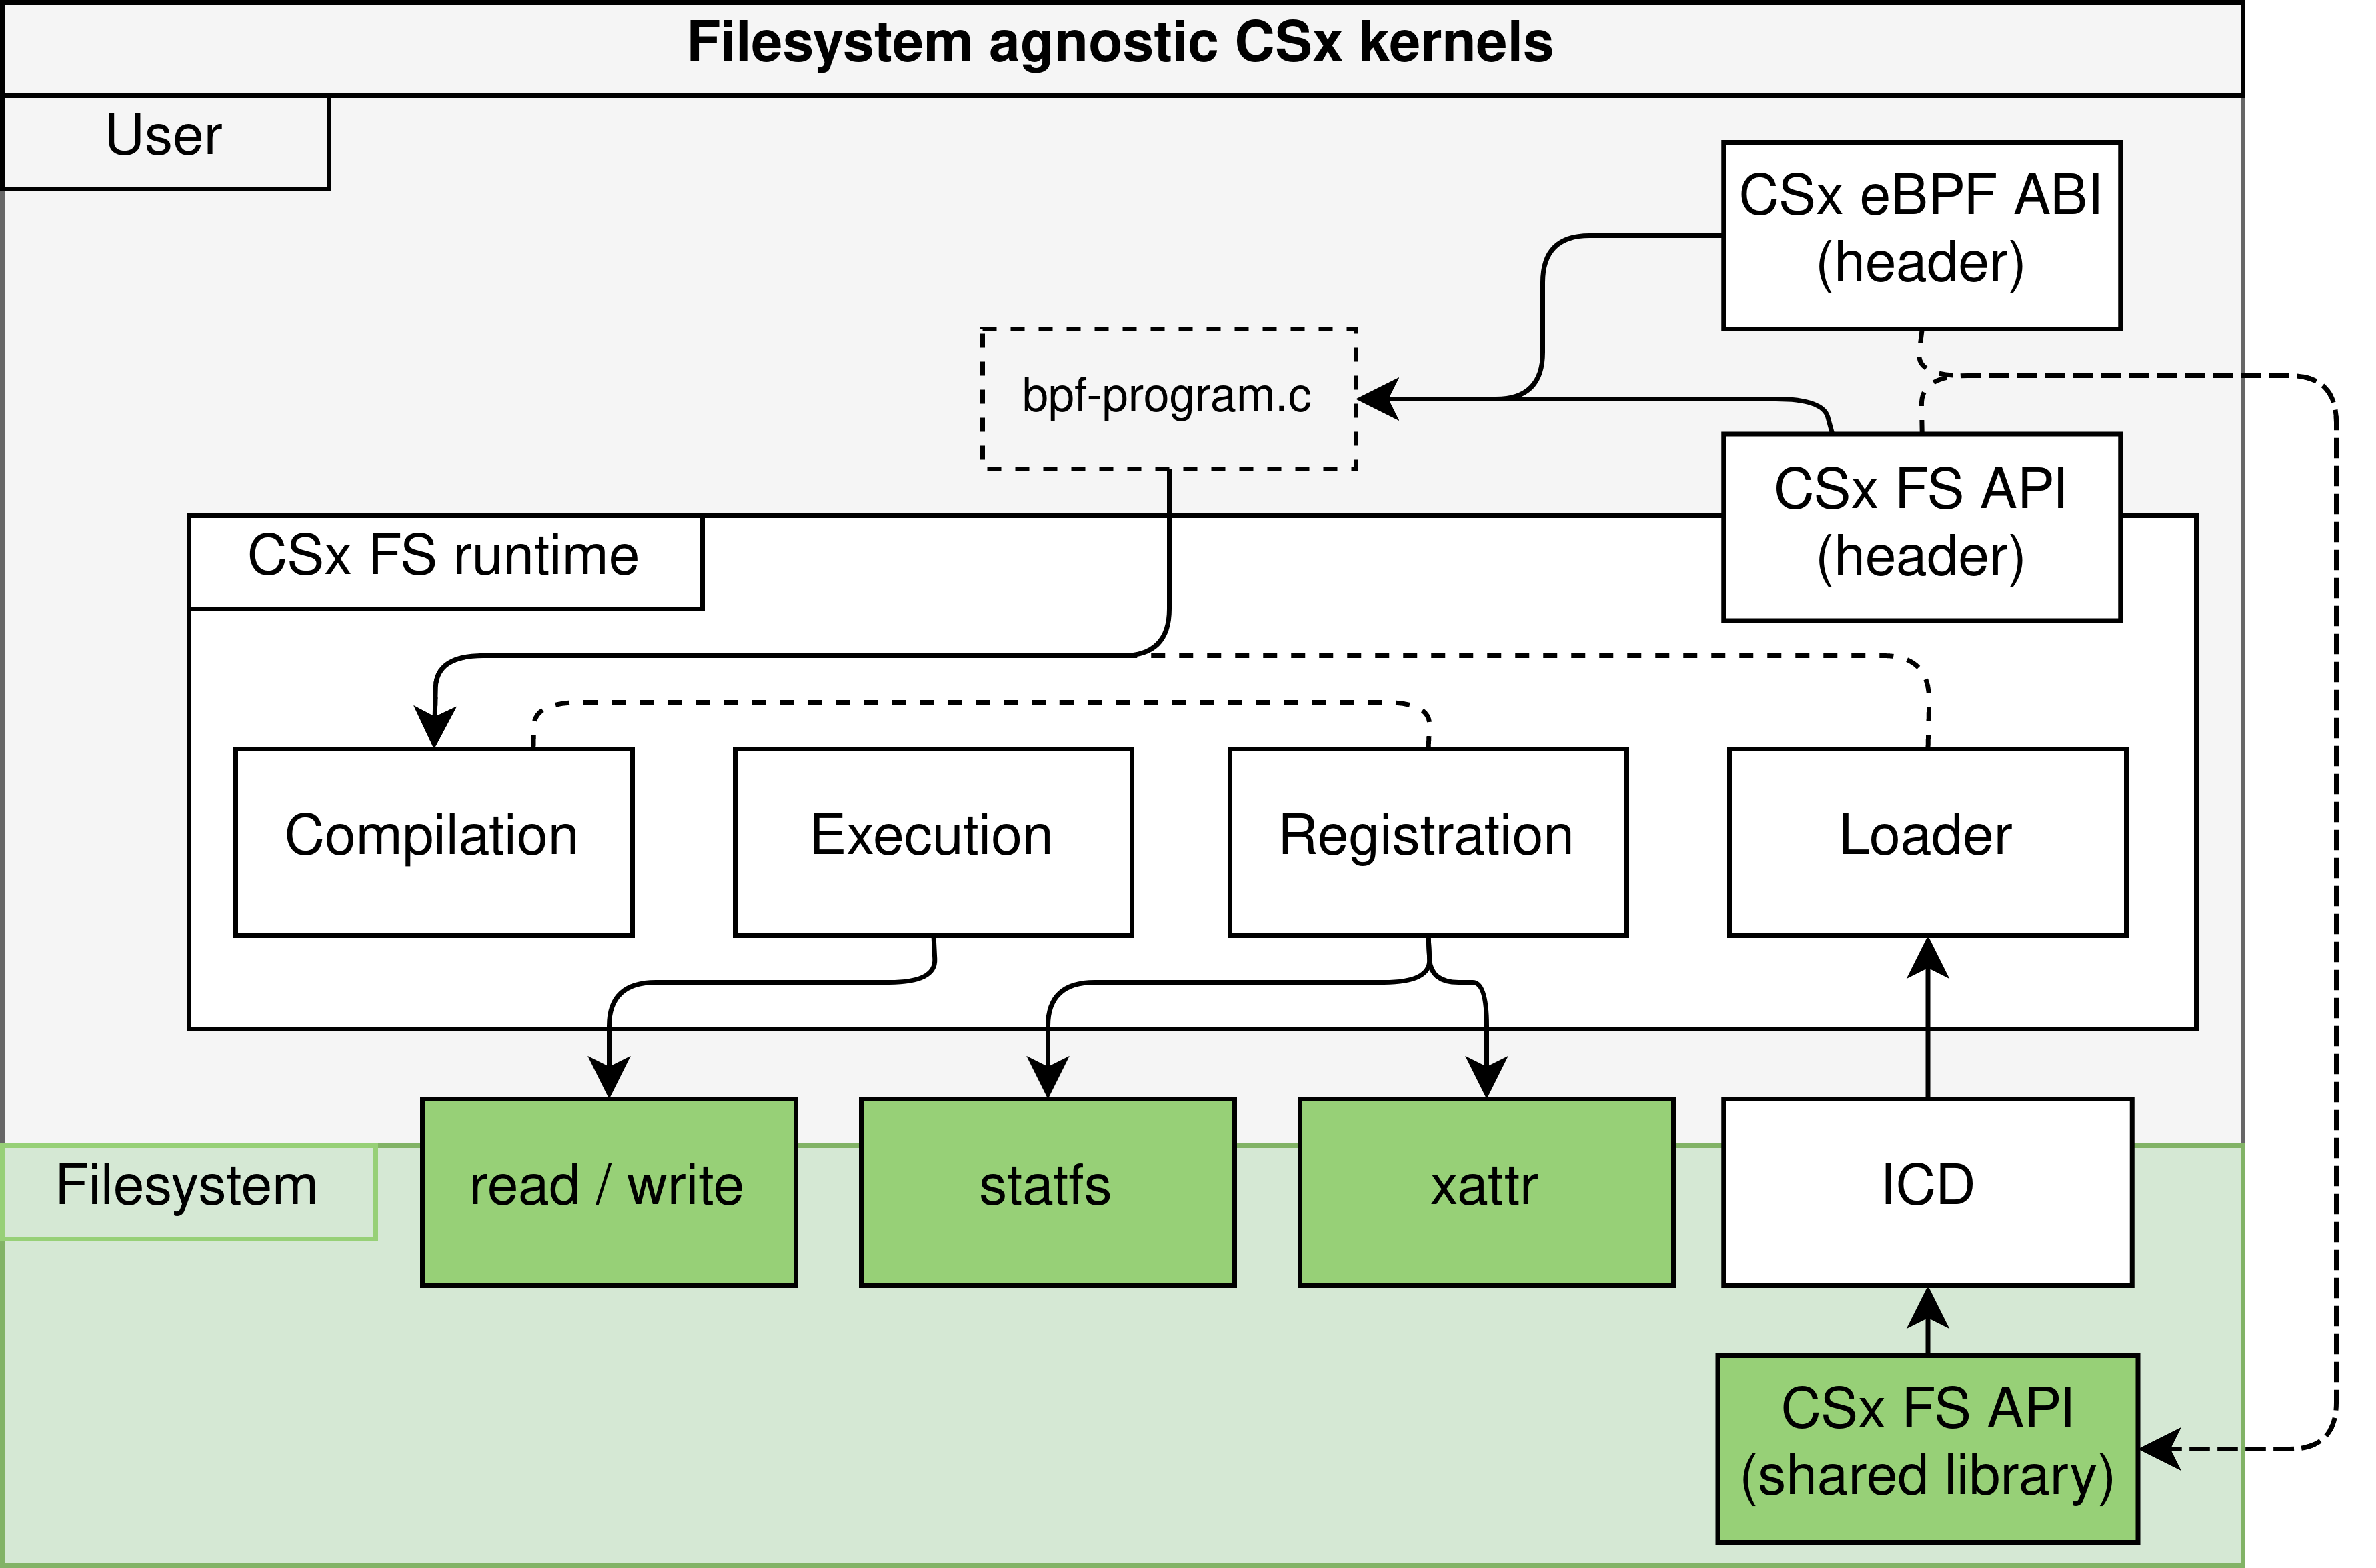
\includegraphics[width=0.8\textwidth]{resources/images/csx-fs-agnostic.png}
% 	% \end{figure}
% 	\endgroup
% \end{frame}

% page 19
\begin{frame}{Limitations}
	\begingroup
	\small
	\begin{itemize}
		\item State of the filesystem
		\item Kernel request stride
		\item Filesystem agnostic kernels
	\end{itemize}
	\endgroup
\end{frame}

% page 20
\begin{frame}{Filesystem Agnostic Kernels}
	\begingroup
	\begin{figure}
		\centering
		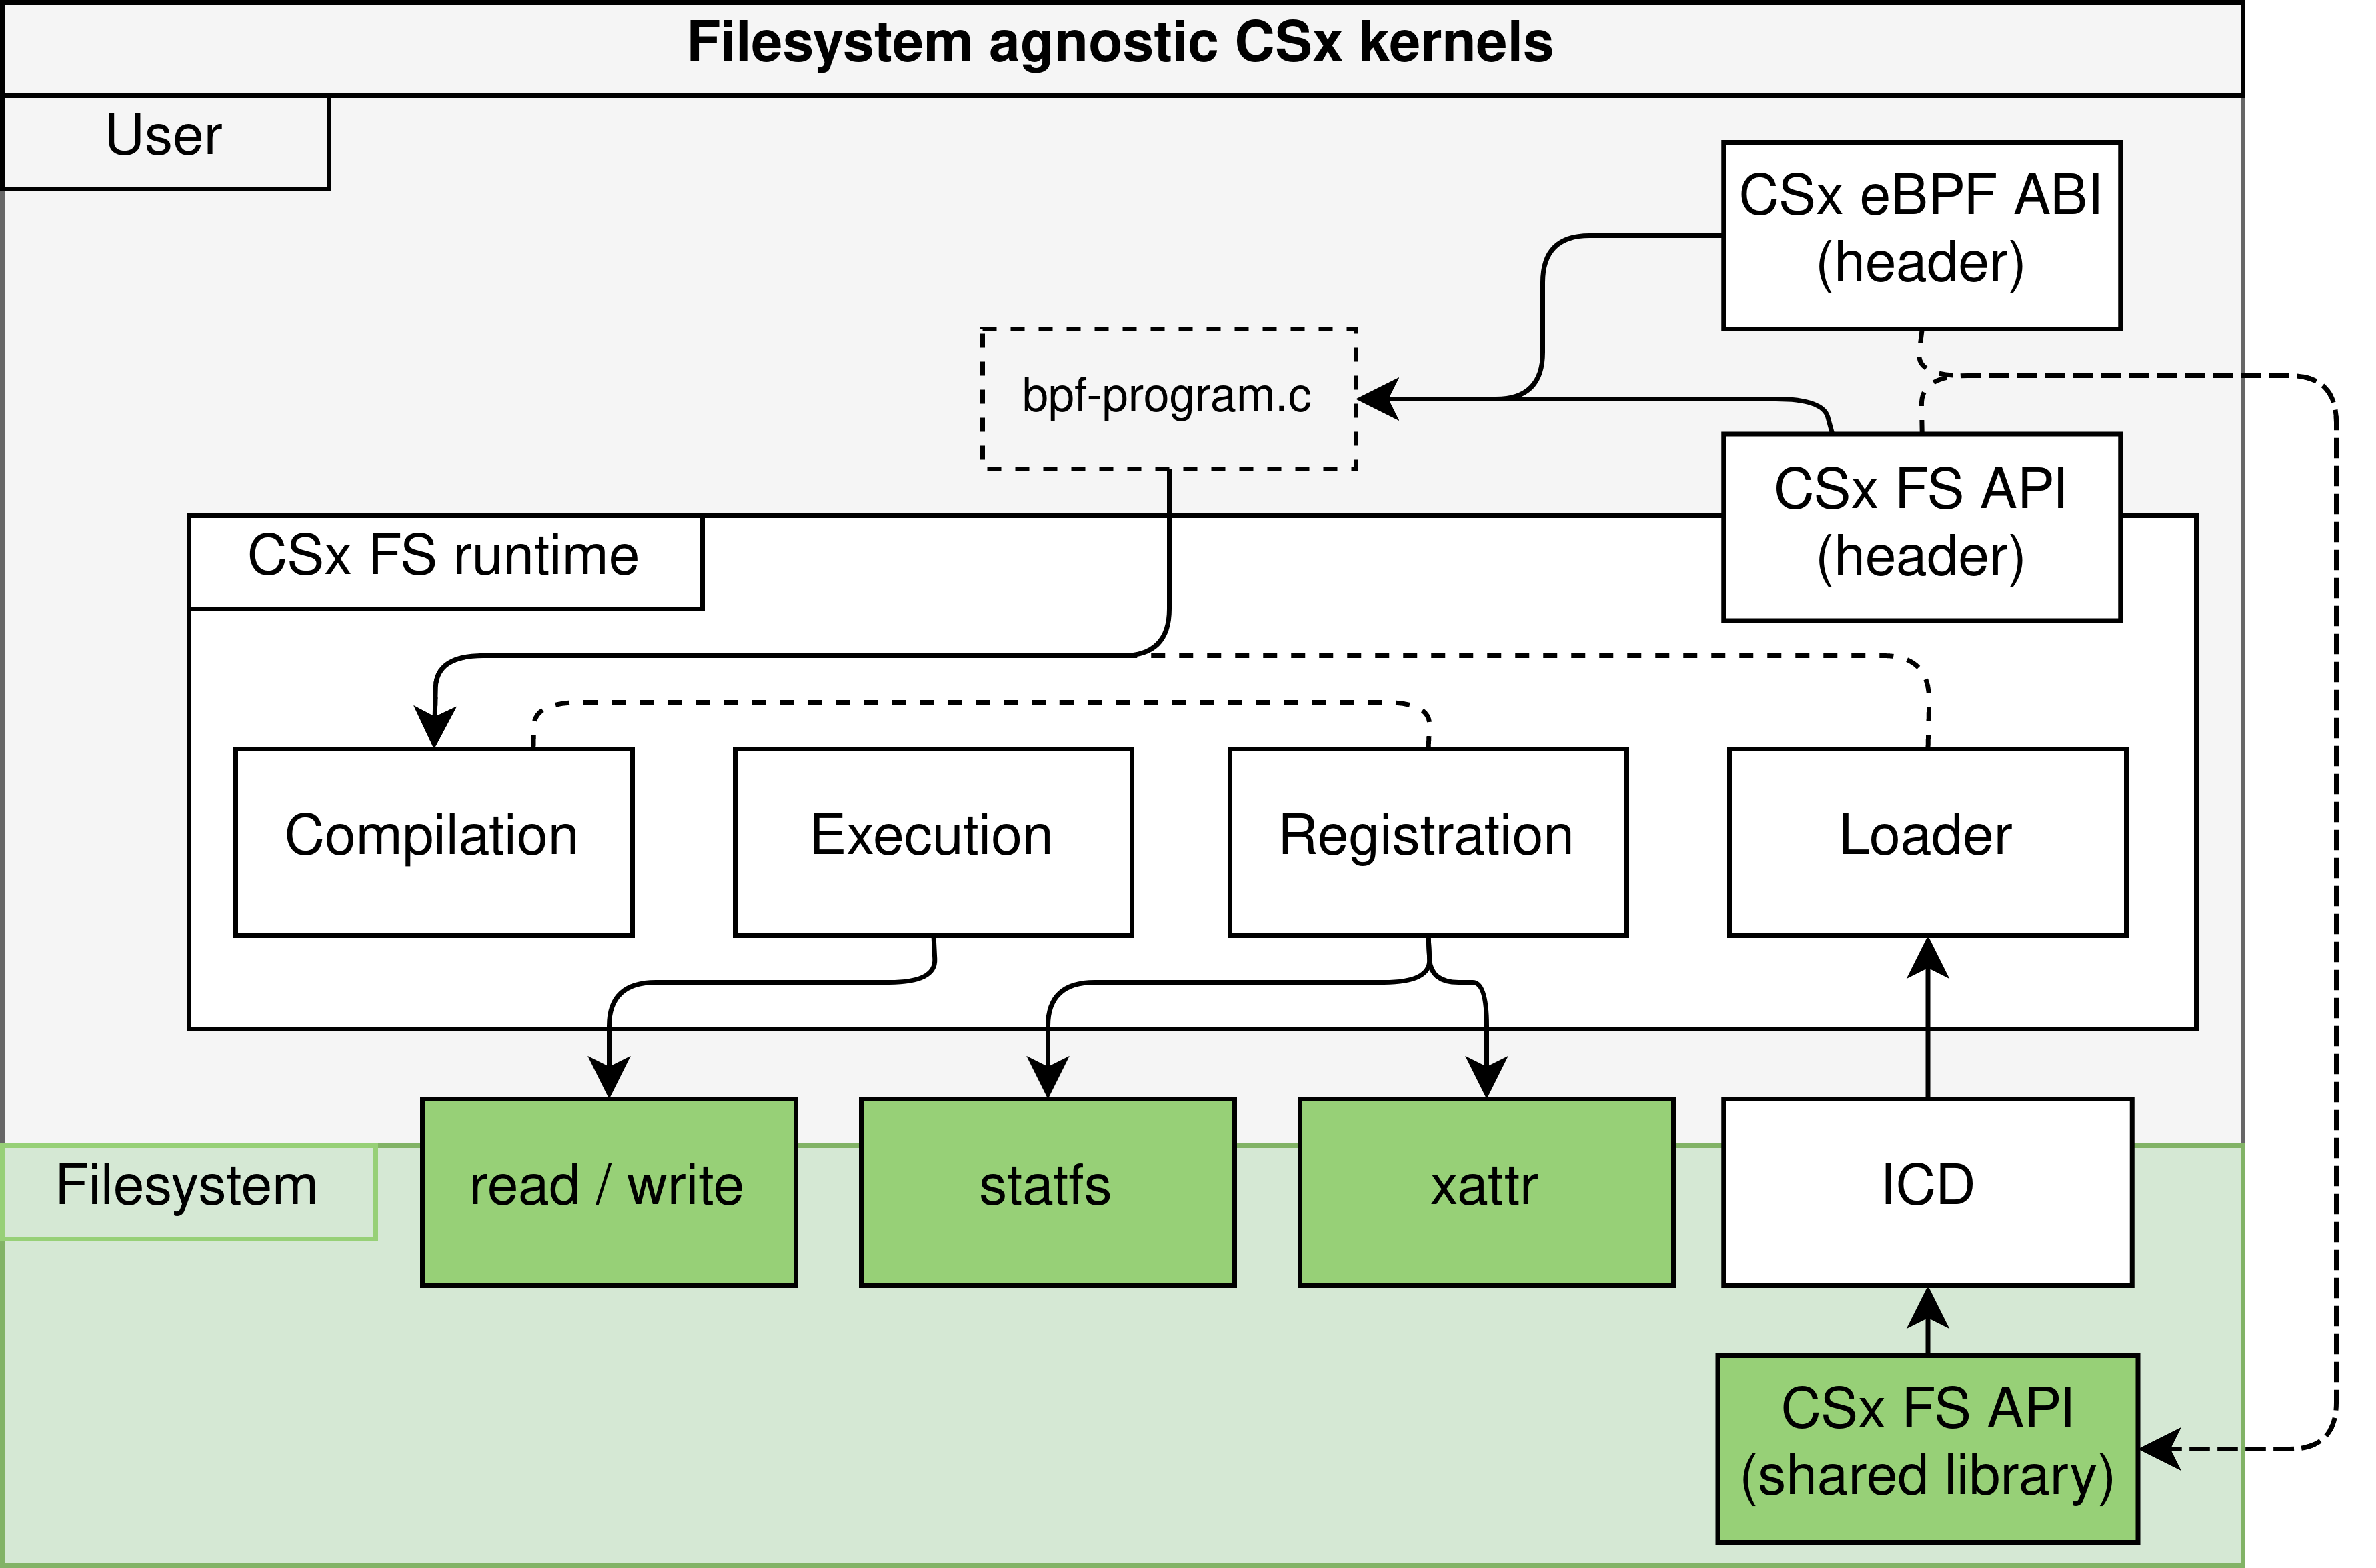
\includegraphics[width=0.8\textwidth]{resources/images/csx-fs-agnostic.png}
	\end{figure}
	\endgroup
\end{frame}

% page 21
\begin{frame}{Conclusion}
	\begingroup
	\small
	\begin{itemize}
		\item Demonstrated \textit{hybrid} filesystem design and implementation
		\item Demonstrated benefits of concurrent background offloading
		\item Many further research venues
		\begin{itemize}
			\item Steady state filesystem
			\item Queue depth beyond  1
			\item Scale offloading performance to embedded platforms
		\end{itemize}
	\end{itemize}
	\endgroup
\end{frame}

% page 22
% All software and data to this project is open source, this includes scripts to
% perform measurements, raw measurement data, scripts to generate graphs and
% even source files to this very presentation. We heavily encourage anyone to
% try it today, there is an extensive readme which includes a video on how to
% setup the project and the source code is extensively documented as well.
% I can not stress enough how important I think this sort of openenness is
% for the reproducability in computer science research. In highly encourage
% everyone to re-evelauate what they are doing to ensure others can reproduce
% their works as well. Thanks you for listening.
\begin{frame}{Further Reading}
	\begingroup
	\small Try it today! \underline{\url{https://github.com/Dantali0n/qemu-csd}}
	\begin{itemize}
		\item OpenCSD: Log-Structured Filesystem enabled Computational
		Storage Device platform - https://tinyurl.com/opencsd-thesis
		\item ICTOPEN: 
		\item ZCSD: a Computational Storage Device over Zoned Namespaces (ZNS)
			SSDs - https://arxiv.org/abs/2112.00142
		\item Past, Present and Future of Computational Storage: A Survey
			- https://arxiv.org/abs/2112.09691
	\end{itemize}
	\endgroup
\end{frame}

% Bonus 1: Related Work
% 
\begin{frame}{Related Work}
	\begingroup
	\begin{figure}
		\centering
		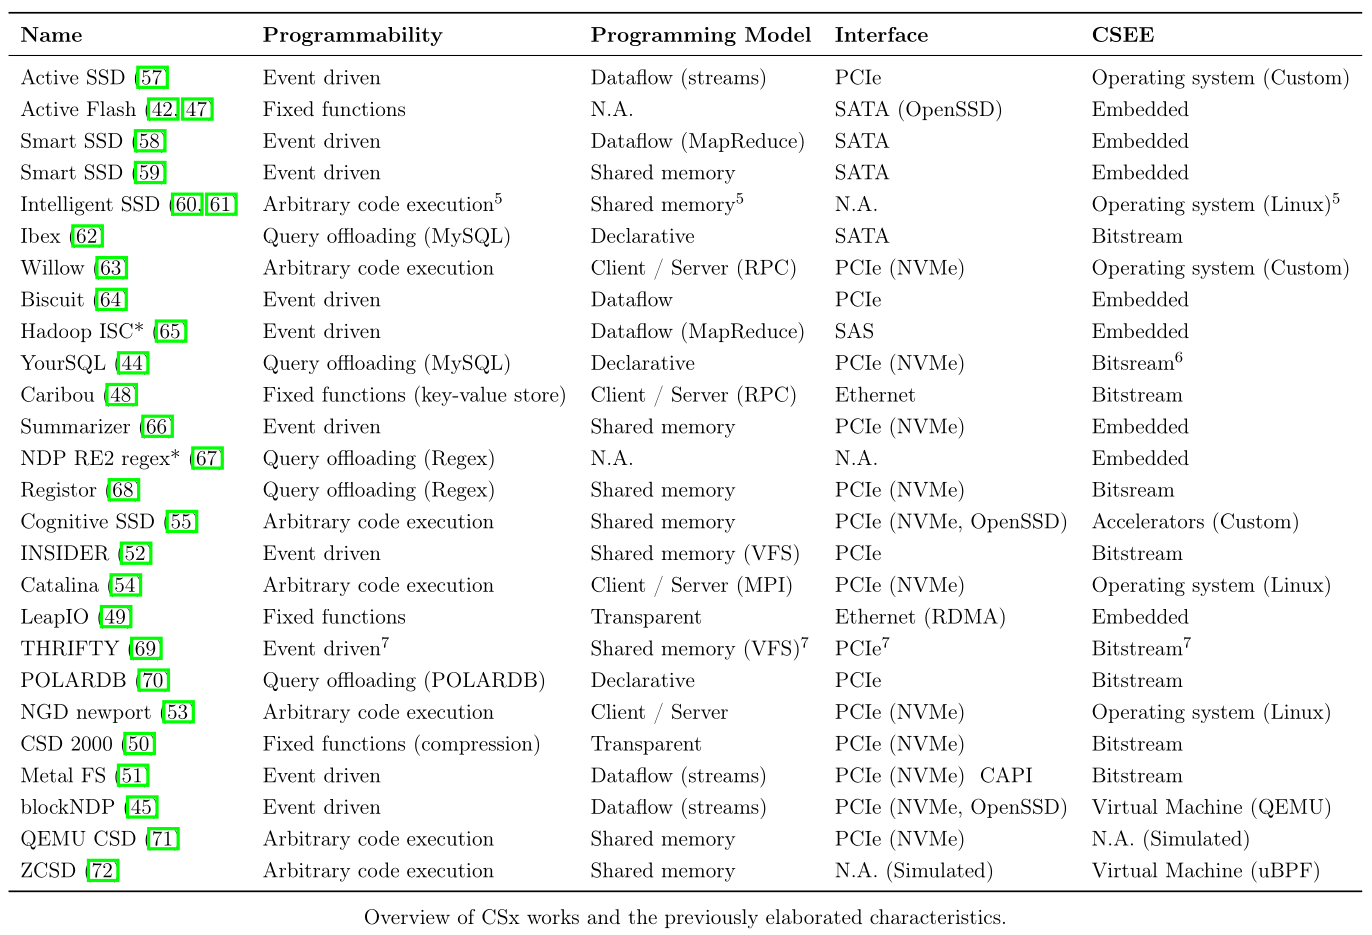
\includegraphics[width=0.9\textwidth]{resources/images/related-work.png}
	\end{figure}
	\endgroup
\end{frame}

% Bonus 2: Scale of the problem
% 
\begin{frame}{Storage Bottleneck}
	\begingroup
	\begin{figure}
		\centering
		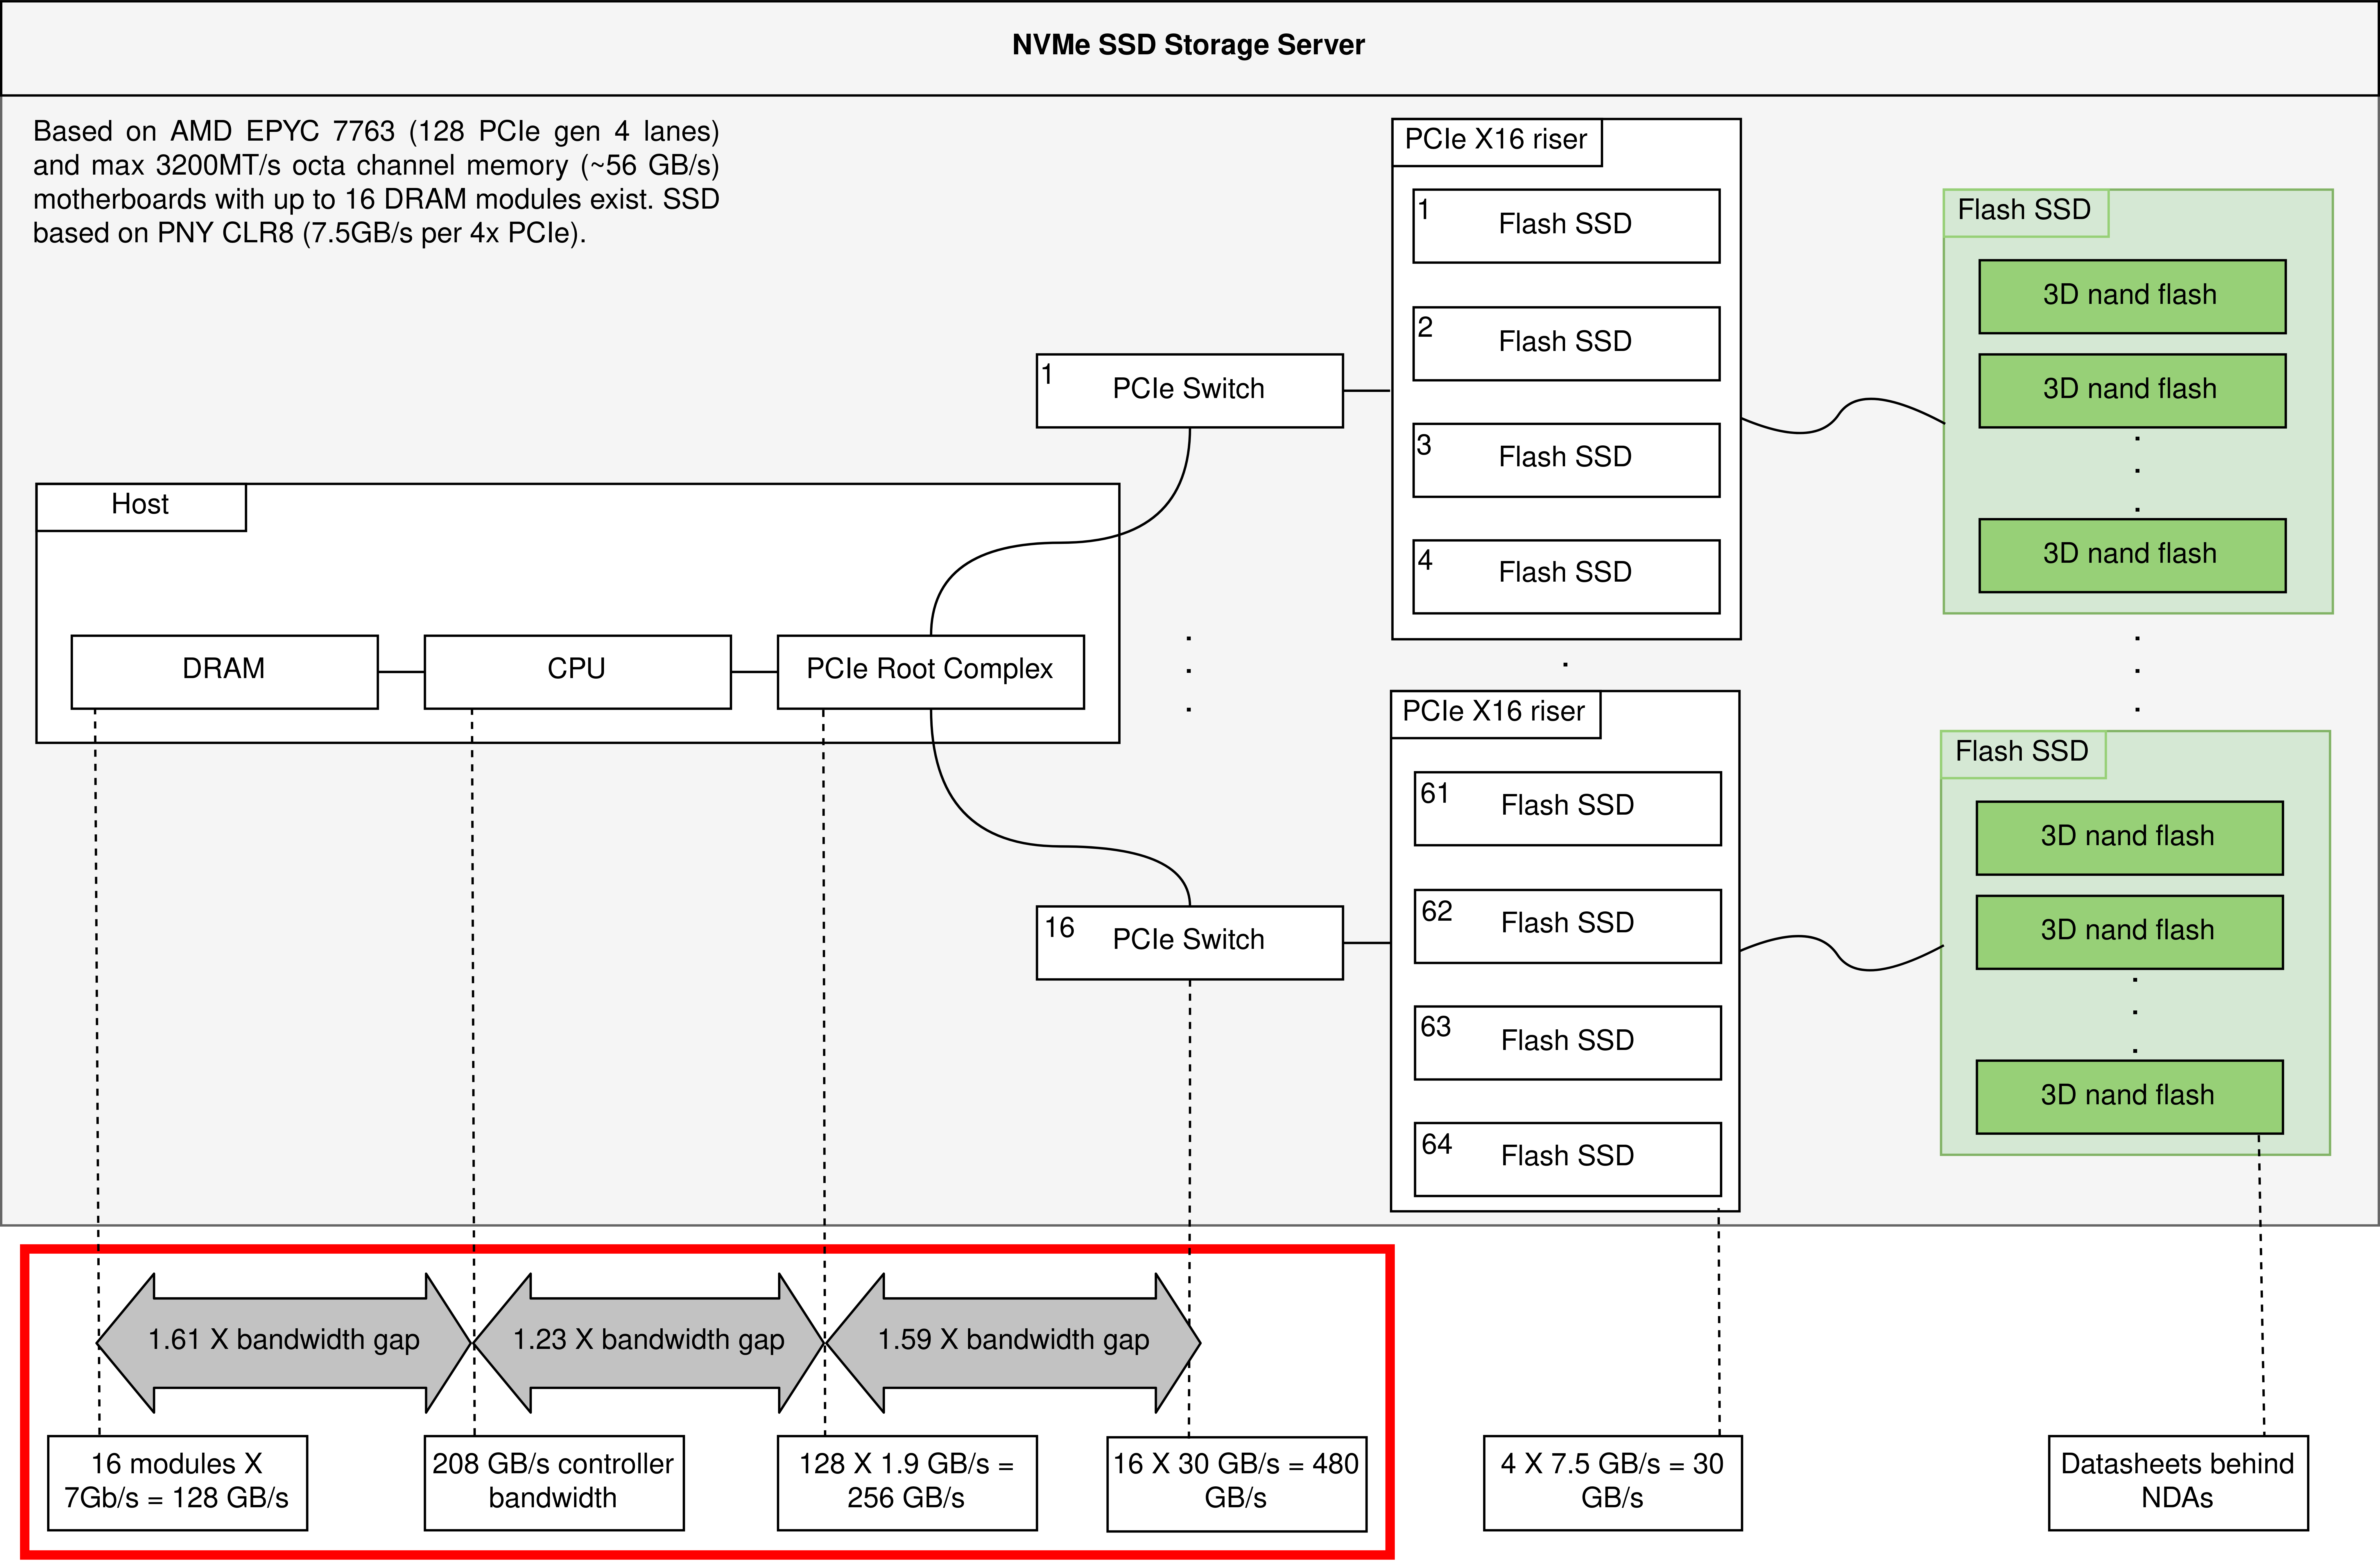
\includegraphics[width=0.9\textwidth]{resources/images/storage-bottleneck.png}
	\end{figure}
	\endgroup
\end{frame}

% Bonus 3: eBPF complex view
% 
\begin{frame}{eBPF with uBPF}
	\begingroup
	\begin{figure}
		\centering
		\includegraphics[width=0.7\textwidth]{resources/images/ubpf-abi.pdf}
	\end{figure}
	\endgroup
\end{frame}

% Bonus 4: questions 
% 
\begin{frame}{Remaining Research Questions}
	\begingroup
	\small
	Design Requirements
	\begin{itemize}
		\item What existing technologies are best suited for a hybrid LFS?
		\item What techniques can be used to minimize the complexity required to
			  use a hybrid LFS?
		\item How to design a compute kernel API that can be reused across
			  devices?
		\item How to ensure user submitted CSx compute kernels are safe?
	\end{itemize}
	Experimental Evaluation
	\begin{itemize}
		\item Can a multi-user tenant hybrid LFS achieve unstagnated performance
			for concurrent regular and offloaded file access?
		\item Can a multi-user tenant hybrid LFS reduce the data movement
			between device and host?
	\end{itemize}
	\endgroup
\end{frame}


\end{document}